\documentclass{Report}

%% Don't import the header multiple times

\ifdefined\HEADERIMPORTED
\else
\newcommand\HEADERIMPORTED[0]{This file is HEADERIMPORTED}
\usepackage{amssymb}

\usepackage{amsmath}


% For typesetting tree rules
\usepackage{mathpartir}

% For colouring code
\usepackage{xcolor}


\usepackage{array}   % for \newcolumntype macro
\usepackage{tikz-cd}
\usepackage{tabstackengine}
\usepackage{breqn}
\usepackage{stmaryrd}

\usepackage{float} % extra options for figure placement

% For drawing boxed
\usepackage{framed}

% for code fragments + highlighting
\usepackage{listings}

% For roman numerals
\usepackage{enumitem}


\usepackage{amsthm}
%Theorems
\usepackage[utf8]{inputenc}
\usepackage[english]{babel}

\ifdefined\PRESENTATIONMODE
\else
\usepackage[a4paper,includeheadfoot,margin=2.54cm]{geometry}
\newtheorem{theorem}{Theorem}[section]
\newtheorem{corollary}{Corollary}[theorem]
\newtheorem{lemma}[theorem]{Lemma}
\newtheorem{definition}{Definition}[section]

\newtheorem{aside}{Aside}[section]
\newtheorem{property}[theorem]{Property}
\theoremstyle{definition}
\fi



\usepackage{tikz}

\definecolor{grey}{rgb}{0.75, 0.75, 0.75}
\definecolor{DarkGreen}{rgb}{0.1, 0.6, 0.1}

\usetikzlibrary{shapes.geometric,fit}
\usetikzlibrary{arrows,automata,positioning}
\usetikzlibrary{decorations.pathreplacing,calc}



\setstackEOL{\cr}
\setstackgap{L}{\normalbaselineskip}

\newcommand\todo[1]{\textbf{TODO: #1}}
\newcommand\needsRef[1]{\textbf{Reference Needed: (#1)}}
\newcommand\fixLayout[1]{\textbf{Fix Layout: #1}}


%% Rule Names
% Prefixes
\newcommand{\tprefix}[0]{T-}
\newcommand{\eprefix}[0]{E-}
\newcommand{\sprefix}[0]{S-}
\newcommand\equationalprefix[0]{Eq-}
\newcommand\envprefix[0]{Env-}
\newcommand\pprefix[0]{\eprefix\envprefix}

\newcommand\subprefix[0]{Sb-}
\newcommand\weakenprefix[0]{Wk-}

% Base  rule names
\newcommand\basenil[0]{Nil}
\newcommand\baseextend[0]{Extend}

\newcommand{\baseground}[0]{Ground}
\newcommand{\baseweaken}[0]{Weaken}
\newcommand{\basevar}[0]{Var}
\newcommand\basefn[0]{Fn}
\newcommand\baseeffect[0]{Effect}
\newcommand\basequant[0]{Quantification}


\newcommand\baseunit[0]{Unit}
\newcommand\basetrue[0]{True}
\newcommand\basefalse[0]{False}
\newcommand\baseconst[0]{Const}
\newcommand\basesubtype[0]{Subtype}
\newcommand\basegen[0]{Effect-Gen}
\newcommand\basespec[0]{Effect-Spec}
\newcommand\basereturn[0]{Return}
\newcommand\baseapply[0]{Apply}
\newcommand\baseif[0]{If}
\newcommand\basebind[0]{Bind}

\newcommand\basetransitive[0]{Transitive}
\newcommand\basereflexive[0]{Reflexive}

\newcommand{\baseid}[0]{Id}
\newcommand\baseproject[0]{Project}

% Effect Weakening Rule Names
\newcommand{\eid}[0]{\eprefix\baseid}
\newcommand{\eproject}[0]{\eprefix\baseproject}
\newcommand{\eextend}[0]{\eprefix\baseextend}

% Term Weakening Rule Names
\newcommand{\tid}[0]{\tprefix\baseid}
\newcommand{\tproject}[0]{\tprefix\baseproject}
\newcommand{\textend}[0]{\tprefix\baseextend}

% Effect Substitution Rule Names
\newcommand\esubnil[0]{\eprefix\basenil}
\newcommand\esubextend[0]{\eprefix\baseextend}

% Term Substitution Rule Names

\newcommand\tsubnil[0]{\tprefix\basenil}
\newcommand\tsubextend[0]{\tprefix\baseextend}

% Type environment Rule Names
\newcommand\envnil[0]{\envprefix\basenil}
\newcommand\envextend[0]{\envprefix\baseextend}
% Effect Environment rule names
\newcommand\pnil[0]{\pprefix\basenil}
\newcommand\pextend[0]{\pprefix\baseextend}
% Equational equality rule names
\newcommand{\eqbeta}[0]{\equationalprefix Lambda-Beta}
\newcommand{\eqeta}[0]{\equationalprefix Lambda-Eta}
\newcommand{\eqeffbeta}[0]{\equationalprefix Effect-Beta}
\newcommand{\eqeffeta}[0]{\equationalprefix Effect-Eta}
\newcommand\eqleftunit[0]{\equationalprefix Left-Unit}
\newcommand\eqrightunit[0]{\equationalprefix Right-Unit}
\newcommand\equnitequiv[0]{\equationalprefix Unit}
\newcommand\eqiftrue[0]{\equationalprefix If-True}
\newcommand\eqiffalse[0]{\equationalprefix If-False}
\newcommand\eqifeta[0]{\equationalprefix If-Eta}
\newcommand\eqassociativity[0]{\equationalprefix Associativity}

\newcommand{\eqreflexive}[0]{\equationalprefix\basereflexive}
\newcommand\eqtransitive[0]{\equationalprefix\basetransitive}
\newcommand\eqsymmetric[0]{\equationalprefix Symmetric}

\newcommand\equnit[0]{\equationalprefix\baseunit}
\newcommand\eqtrue[0]{\equationalprefix\basetrue}
\newcommand\eqfalse[0]{\equationalprefix\basefalse}
\newcommand\eqconst[0]{\equationalprefix\baseconst}
\newcommand{\eqvar}[0]{\equationalprefix\basevar}
\newcommand\eqweaken[0]{\equationalprefix\baseweaken}
\newcommand\eqfun[0]{\equationalprefix\basefn}
\newcommand\eqsubtype[0]{\equationalprefix\basesubtype}
\newcommand\eqgen[0]{\equationalprefix\basegen}
\newcommand\eqspec[0]{\equationalprefix\basespec}
\newcommand\eqreturn[0]{\equationalprefix\basereturn}
\newcommand\eqapply[0]{\equationalprefix\baseapply}
\newcommand\eqif[0]{\equationalprefix\baseif}
\newcommand\eqbind[0]{\equationalprefix\basebind}

% Term rule names
\newcommand\vunit[0]{\baseunit}
\newcommand\vtrue[0]{\basetrue}
\newcommand\vfalse[0]{\basefalse}
\newcommand\vconst[0]{\baseconst}
\newcommand{\vvar}[0]{\basevar}
\newcommand\vweaken[0]{\baseweaken}
\newcommand\vfun[0]{\basefn}
\newcommand\vsubtype[0]{\basesubtype}
\newcommand\vgen[0]{\basegen}
\newcommand\vspec[0]{\basespec}
\newcommand\vreturn[0]{\basereturn}
\newcommand\vapply[0]{\baseapply}
\newcommand\vif[0]{\baseif}
\newcommand\vbind[0]{\basebind}

%Effect rule names
\newcommand\eground[0]{\eprefix\baseground}
\newcommand\evar[0]{\eprefix\basevar}
\newcommand\eweaken[0]{\eprefix\baseweaken}
\newcommand\ecompose[0]{\eprefix Compose}

% Type rule names
\newcommand{\tground}[0]{\tprefix\baseground}
\newcommand{\tfun}[0]{\tprefix\basefn}
\newcommand{\teffect}[0]{\tprefix\baseeffect}
\newcommand{\tquant}[0]{\tprefix\basequant}

% Subtyping rule names
\newcommand{\stransitive}[0]{\sprefix\basetransitive}
\newcommand{\sreflexive}[0]{\sprefix\basereflexive}
\newcommand{\sground}[0]{\sprefix\baseground}
\newcommand{\sfun}[0]{\sprefix\basefn}
\newcommand{\seffect}[0]{\sprefix\baseeffect}
\newcommand{\squant}[0]{\sprefix\basequant}


\newcommand{\s}{\;}
\newcommand{\doin}[3]{\texttt{do}\s #1 \leftarrow #2 \s\texttt{in}\s #3\s}
\newcommand\apply[2]{#1\s#2}
\newcommand{\pifthenelse}[4]{\texttt{if}_{\textcolor{purple}{#1}}\s#2\s \texttt{then}\s #3 \s\texttt{else} \s#4\s}
\newcommand\ifthenelse[5]{\pifthenelse{#1, #2}{#3}{#4}{#5}}
\newcommand\const[1]{\texttt{k}^{\color{purple} #1}}
\newcommand\return[1]{\texttt{return} \s#1\s}


\newcommand\lam[3]{\lambda #1 \colon {\color{purple}#2}. #3\s}
\renewcommand\u[0]{\texttt{()}}
\newcommand{\U}[0]{\texttt{Unit}}
\renewcommand\t[0]{\texttt{true}}
\newcommand\f[0]{\texttt{false}}
\newcommand{\B}[0]{\texttt{Bool}}
\newcommand{\G}[0]{\Gamma}
\newcommand\D{\Delta}


% draw type relations
\newcommand{\typerelation}[3]{{\color{DarkGreen}#1} \vdash #2 \colon {\color{blue}#3}}
\newcommand\wellformed[2]{{\color{DarkGreen}#1}\vdash {\color{blue}#2}}
\newcommand\wellformedok[2]{\ok{{\color{DarkGreen}#1}\vdash {\color{blue} #2}}}

\newcommand{\wellformedtype}[2]{\typerelation{#1}{#2}{\type}}
\newcommand{\wellformedeffect}[2]{\typerelation{#1}{#2}{\effect}}
\newcommand{\wellformedF}[2]{\typerelation{#1}{#2}{F}}



\newcommand{\gtyperelation}[2]{\typerelation{\G}{#1}{#2}}
 

\newcommand\treerulez[1]{\inferrule{ }{#1}}
\newcommand\treeruleI[2]{\inferrule{#1}{#2}}
\newcommand\treeruleII[3]{\inferrule{#1 \\ #2}{#3}}
\newcommand\treeruleIII[4]{\inferrule{#1 \\ #2 \\ #3}{#4}}
\newcommand\treeruleIV[5]{\inferrule{#1 \\ #2 \\ #3 \\ #4}{#5}}
\newcommand\treeruleV[6]{\inferrule{#1 \\ #2 \\ #3 \\ #4 \\ #5}{#6}}

\newcommand\ntreerulez[2]{(\text{#1})\inferrule{ }{#2}}
\newcommand\ntreeruleI[3]{(\text{#1})\inferrule{#2}{#3}}
\newcommand\ntreeruleII[4]{(\text{#1})\inferrule{#2 \\ #3}{#4}}
\newcommand\ntreeruleIII[5]{(\text{#1})\inferrule{#2 \\ #3 \\ #4}{#5}}
\newcommand\ntreeruleIV[6]{(\text{#1})\inferrule{#2 \\ #3 \\ #4 \\ #5}{#6}}
\newcommand\ntreeruleV[7]{(\text{#1})\inferrule{#2 \\ #3 \\ #4 \\ #5 \\ #6}{#7}}

\newcommand\condtreerulez[3]{(\text{#1})\inferrule{ }{#2}(\text{if } #3)}
\newcommand\condtreeruleI[4]{(\text{#1})\inferrule{#2}{#3}(\text{if } #4)}
\newcommand\condtreeruleII[5]{(\text{#1})\inferrule{#2 \\ #3}{#4}(\text{if } #5)}
\newcommand\condtreeruleIII[6]{(\text{#1})\inferrule{#2 \\ #3 \\ #4}{#5}(\text{if } #6)}
\newcommand\condtreeruleIV[7]{(\text{#1})\inferrule{#2 \\ #3 \\ #4 \\ #5}{#6}(\text{if } #7)}
\newcommand\condtreeruleV[8]{(\text{#1})\inferrule{ #2 \\ #3 \\ #4 \\ #5 \\ #6 }{#7}(\text{if } #8)}



\newcommand{\subtype}[0]{\leq\colon}
\newcommand\subeffect[0]{\leq}

\newcommand{\M}[2]{\texttt{M}_{#1}{#2}}

\newcommand\lamtype[3]{#1 \rightarrow \M{#2}{#3}}
\newcommand{\1}[0]{\texttt{1}}

\newcommand\e[0]{\epsilon}

\newcommand{\db}[1]{{\bf [\![}#1{\bf ]\!]}}
\newcommand{\deno}[1]{\db{#1}}
\newcommand\after\circ
\newcommand\term[1]{\langle\rangle_{#1}}

\newcommand\bindmu[0]{\mu}
\newcommand\point[1]{\eta_{#1}}
\newcommand\bind[3]{\bindmu_{#1, #2, #3}}

\newcommand\T[2]{T_{#1}{#2}}

\newcommand\pr[2]{\langle#1, #2\rangle}
\newcommand\finpr[2]{\langle #1\rangle_{#2}}

\newcommand\strengtht[0]{\texttt{t}}
% tensor strength Nat-tran
\newcommand\tstrength[3]{\strengtht_{#1, #2, #3}}

% Id morphism
\newcommand\Id[1]{\texttt{Id}_{#1}}

\newcommand\idg[0]{\Id{\G}}
% beta-eta equivalence
\newcommand\beequiv[0]{\approx}
% Substitutions
\newcommand\si{\sigma}

\newcommand{\sub}[1]{[#1]}
\newcommand{\ssub}[2]{[#2 / #1]}
\newcommand{\ssi}[0]{\sub{\si}}

% beta-eta equivalence relation
\newcommand{\berelation}[4]{\typerelation{#1}{#2 \beequiv #3}{#4}}
\newcommand{\gberelation}[3]{\gtyperelation{#1 \beequiv #2}{#3}}


% Shortcuts for denotational equality
\newcommand{\denoequality}[4]{\deno{\typerelation{#1}{#2}{#4}} = \deno{\typerelation{#1}{#3}{#4}}}
\newcommand{\gdenoequality}[3]{\denoequality{\G}{#1}{#2}{#3}}

% Shorthand for monad types
\newcommand\mea[0]{\M{\e}{A}}
\newcommand\meb[0]{\M{\e}{B}}
\newcommand\mec[0]{\M{\e}{C}}

\newcommand\tea[0]{\T{\e}{A}}
\newcommand\teb[0]{\T{\e}{B}}
\newcommand\tec[0]{\T{\e}{C}}


\newcommand\moa[0]{\M{\1}{A}}
\newcommand\mob[0]{\M{\1}{B}}
\newcommand\moc[0]{\M{\1}{C}}

\newcommand\toa[0]{\T{\1}{A}}
\newcommand\tob[0]{\T{\1}{B}}
\newcommand\toc[0]{\T{\1}{C}}

\newcommand\aeb[0]{\lamtype{A}{\e}{B}}

% Shorthand for Gammas
\newcommand{\gax}[0]{\G, x\colon A}
\newcommand{\gby}[0]{\G, y\colon B}

% reduction function
\newcommand{\reduce}[0]{reduce}



% Combinators for building delta-based tree proof terms
\newcommand{\deltavrule}[4]{
    \ntreeruleII{\vsubtype}{\treeruleI{\D}{\typerelation{#1}{#2}{#3}}}{#3 \subtype #4}{\typerelation{#1}{#2}{#4}}}

\newcommand{\deltavruleprime}[4]{
    \ntreeruleII{\vsubtype}{\treeruleI{\D'}{\typerelation{#1}{#2}{#3}}}{#3 \subtype #4}{\typerelation{#1}{#2}{#4}}}

\newcommand{\deltavruleprimeprime}[4]{
        \ntreeruleII{\vsubtype}{\treeruleI{\D'}{\typerelation{#1}{#2}{#3}}}{#3 \subtype #4}{\typerelation{#1}{#2}{#4}}}
    
\newcommand{\deltacrule}[6]{
            \ntreeruleII{Subeffect}{\treeruleI{\D}{\typerelation{#1}{#2}{\M{#3}{#4}}}}{\subeffecttree{#3}{#4}{#5}{#6}}{\typerelation{#1}{#2}{\M{#5}{#6}}}}
\newcommand{\deltacruleprime}[6]{
    \ntreeruleII{Subeffect}{\treeruleI{\D'}{\typerelation{#1}{#2}{\M{#3}{#4}}}}{
    \subeffecttree{#3}{#4}{#5}{#6}}{\typerelation{#1}{#2}{\M{#5}{#6}}}}
\newcommand{\deltacruleprimeprime}[6]{
    \ntreeruleII{\vsubtype}{\treeruleI{\D''}{\typerelation{#1}{#2}{\M{#3}{#4}}}}{
        \subeffecttree{#3}{#4}{#5}{#6}}{\typerelation{#1}{#2}{\M{#5}{#6}}}}
                            

\newcommand{\p}[0]{\pi_1}
\newcommand{\pp}[0]{\pi_2}

% short-hands for weakening
\newcommand{\wrel}[3]{#1 \colon {\color{blue}#2} \triangleright {\color {blue} #3}}
\newcommand{\ok}[1]{{\color{blue} #1} \texttt{ Ok}}
\newcommand\okt[0]{\texttt{Ok}}
\renewcommand\i[0]{\iota}
\newcommand\w{\omega}
\newcommand\dom[1]{\texttt{dom}(#1)}
\newcommand\x{\times}


\newcommand\fev[1]{fev(#1)}
\newcommand\union[0]{\cup}


% Combinators to build tree proofs
\newcommand{\truleconst}[0]{\ntreeruleI{\vconst}{\ok{\G}}{\gtyperelation{\const{A}}{A}}}
\newcommand{\truleunit}[0]{\ntreeruleI{\vunit}{\ok{\G}}{\typerelation{\G}{\u}{\U}}}
\newcommand{\truletrue}[0]{\ntreeruleI{\vtrue}{\ok{\G}}{\typerelation{\G}{\t}{\B}}}
\newcommand{\trulefalse}[0]{\ntreeruleI{\vfalse}{\ok{\G}}{\typerelation{\G}{\f}{\B}}}


\newcommand{\E}[0]{\mathbb{E}}
\renewcommand{\dot}{\cdot}
\newcommand{\gens}[0]{\colon\colon=}
\newcommand{\nil}[0]{\diamond}
\newcommand{\ground}[0]{\gamma}

% Terminal object of C
\newcommand{\terminal}[0]{\texttt{\1}}

% The category C
\newcommand{\C}[0]{\mathbb{C}}
\newcommand{\Cz}[0]{\C_0}
\newcommand\DC[0]{\mathbb{D}}

% The category of locally-small categories
\newcommand{\Cat}[0]{\texttt{Cat}}
% Sub-effect Nat-trans
\newcommand{\dse}[2]{\db{#1 \subeffect #2}}

\newcommand\app[0]{\texttt{app}}
\newcommand\cur[1]{\texttt{cur}(#1)}
\newcommand{\ifnt}[1]{\texttt{If}_{#1}}


\newcommand{\setto}{\colon=}
\newcommand{\fv}[1]{\texttt{fv}(#1)}

% shorthand for inserting text to equations
\newcommand\qt[1]{\quad\text{#1}}

% Co-product short-hands
\newcommand\inr[0]{\texttt{inr}}
\newcommand\inl[0]{\texttt{inl}}
    
\newcommand\fld[2]{[#1,#2]}
\newcommand{\diag}[1]{\delta_{#1}}
\newcommand{\twist}[2]{\tau_{#1, #2}}

\newcommand\ifMorph[3]{\app\after((\fld{\cur{#2\after\pp}}{\cur{#3\after\pp}}\after #1)\times \idg)\after \diag{\G}}


% Polymorphic short-hands
\newcommand\elam[2]{\Lambda #1. #2}
\newcommand{\eapp}[2]{#1\s#2}
\renewcommand{\a}[0]{\alpha}
\newcommand{\all}[2]{\forall #1. #2}
\renewcommand{\P}[0]{\Phi}

\renewcommand{\b}[0]{\beta}
\newcommand{\g}[0]{\gamma}
\renewcommand\d[0]{\delta}
\newcommand\oke[2]{\wellformedok{#1}{#2}}
\newcommand\etyperelation[4]{\typerelation{#1\mid#2}{#3}{#4}}
\newcommand{\gpetyperelation}[2]{\etyperelation{\P}{\G}{#1}{#2}}
\newcommand{\gppetyperelation}[2]{\etyperelation{\P'}{\G}{#1}{#2}}


\newcommand{\eberelation}[5]{\berelation{#1\mid#2}{#3}{#4}{#5}}
\newcommand{\gpeberelation}[3]{\berelation{\P\mid\G}{#1}{#2}{#3}}
\newcommand{\gppeberelation}[3]{\berelation{\P'\mid\G}{#1}{#2}{#3}}

\newcommand{\dotp}[0]{\dot_\P}
\newcommand{\fntype}[2]{#1\rightarrow #2}
\newcommand{\ab}[0]{\fntype{A}{B}}

\newcommand\wrelw[2]{\wrel{\w}{#1}{#2}}
\renewcommand\proof[0]{\paragraph{Proof:}}
\newcommand{\case}[1]{\paragraph{Case #1:}}
\newcommand{\subcase}[1]{\subparagraph{Case: #1}}
\newcommand\bi[0]{By inversion}

%pre-filled effect-weakening relations
\newcommand\ewrel[4]{\wellformed{#1}{\color{black}\wrel{#2}{#3}{#4}}}
\newcommand\pewrel[3]{\ewrel{\P}{#1}{#2}#3}
\newcommand\ppewrel[3]{\ewrel{\P'}{#1}{#2}#3}

\newcommand\subtypep[0]{\subtype_\P}
\newcommand\subtypepp[0]{\subtype_{\P'}}
\newcommand\subeffectp[0]{\subeffect_{\P}}
\newcommand\subeffectpp[0]{\subeffect_{\P'}}
\newcommand\subeffectn[0]{\subeffect_{n}}
\newcommand\subeffectz[0]{\subeffect_{0}}

\newcommand{\allI}[0]{\forall_I}
\newcommand{\allII}[0]{\forall_{I'}}
\newcommand\allIU[0]{\forall_{I\times U}}
\newcommand\type[0]{\texttt{Type}}
\newcommand\effect[0]{\texttt{Effect}}
\newcommand\ciw[0]{\C(I, W)}
\newcommand\ciu[0]{\C(I, U)}
\newcommand\ciuw[0]{\C(I\times U, W)}
\newcommand\cipw[0]{\C(I', W)}
\newcommand\cipu[0]{\C(I', U)}
\newcommand\ciuu[0]{\C(I\times U, U)}
\newcommand\cii[0]{\C(I', I)}
\newcommand\Eff[0]{\texttt{Eff}}
\newcommand\Mul[0]{\texttt{Mul}}
\newcommand\singleton[0]{\ast}
\renewcommand\star[0]{^*}
\renewcommand\bar[1]{\overline{#1}}

\newcommand\subtypeg[0]{\subtype_\g}
\newcommand\subtypepa[0]{\subtype_{\P, \a}}
\newcommand\subtypeppa[0]{\subtype_{\P', \a}}

\newcommand\subtypez[0]{\subtype_{0}}
\newcommand\subtypen[0]{\subtype_{n}}

\usepackage{scalerel,stackengine}
\stackMath
\renewcommand\widehat[1]{%
\savestack{\tmpbox}{\stretchto{%
  \scaleto{%
    \scalerel*[\widthof{\ensuremath{#1}}]{\kern.1pt\mathchar"0362\kern.1pt}%
    {\rule{0ex}{\textheight}}%WIDTH-LIMITED CIRCUMFLEX
  }{\textheight}% 
}{2.4ex}}%
\stackon[-6.9pt]{#1}{\tmpbox}%
}
\parskip 1ex

\newcommand\pstar[0]{\p\star}

\newcommand\edeltavrule[5]{\deltavrule{#1 \mid #2}{#3}{#4}{#5}}

\newcommand\subeffecttreep[4]{\ntreeruleII{\teffect}{
    #1\subeffectp #3}{#2 \subtypep #4
}{\M{#1}{
    #2
}\subtypep\M{#3}{#4}}}
\newcommand\subeffecttree[4]{\ntreeruleII{\teffect}{
    #1\subeffect #3}{#2 \subtype #4
}{\M{#1}{
    #2
}\subtype\M{#3}{#4}}}


\newcommand{\edeltavruleprime}[5]{
        \deltavruleprime{#1\mid #2}{#3}{#4}{#5}}
    
\newcommand{\edeltavruleprimeprime}[5]{
        \deltavruleprimeprime{#1\mid #2}{#3}{#4}{#5}}
    
\newcommand{\edeltacrule}[6]{
            \ntreeruleII{\vsubtype}{
                \treeruleI{
                    \D
                }{
                    \typerelation{\P\mid#1}{#2}{\M{#3}{#4}}
                }
            }{
                \ntreeruleII{\teffect}{
                    #4 \subtypep #6
                    }{
                         #3 \subeffectp #5
                }{
                    \M{#3}{#4}\subtypep{\M{#5}{#6}}
                }
            }{
                \typerelation{\P\mid #1}{#2}{\M{#5}{#6}}
            }
        }
        

        \newcommand{\edeltacruleprime}[6]{
            \ntreeruleII{\vsubtype}{
                \treeruleI{
                    \D'
                }{
                    \typerelation{\P\mid #1}{#2}{\M{#3}{#4}}
                }
            }{
                \ntreeruleII{\teffect}{
                    #4 \subtypep #6
                }{#3 \subeffectp #5
                }{
                    \M{#3}{#4}\subtypep{\M{#5}{#6}}
                }
            }{
                \typerelation{\P\mid #1}{#2}{\M{#5}{#6}}
            }
        }
                   

        \newcommand{\edeltacruleprimeprime}[6]{
            \ntreeruleII{\vsubtype}{
                \treeruleI{
                    \D''
                }{
                    \typerelation{\P\mid #1}{#2}{\M{#3}{#4}}
                }
            }{
                \ntreeruleII{\teffect}{
                    #4 \subtypep #6
                    }{ #3 \subeffectp #5
                }{
                    \M{#3}{#4}\subtypep{\M{#5}{#6}}
                }
            }{
                \typerelation{\P\mid #1}{#2}{\M{#5}{#6}}
            }
        }

        \newcommand\obj[0]{\texttt{obj }}


        \newcommand{\Tz}[2]{\texttt{T}^0_{#1}#2}
        \newcommand{\Tn}[2]{\texttt{T}^n_{#1}#2}
        \newcommand{\Tm}[2]{\texttt{T}^m_{#1}#2}
        
        \newcommand{\pointz}[1]{\point{#1}^0}
        \newcommand{\pointn}[1]{\point{#1}^n}
        \newcommand{\pointm}[1]{\point{#1}^m}
        
        \newcommand{\bindz}[3]{\bind{#1}{#2}{#3}^0}
        \newcommand{\bindn}[3]{\bind{#1}{#2}{#3}^n}
        \newcommand{\bindm}[3]{\bind{#1}{#2}{#3}^m}
        
        \newcommand\tstrengthz[3]{\tstrength{#1}{#2}{#3}^0}
        \newcommand\tstrengthn[3]{\tstrength{#1}{#2}{#3}^n}
        \newcommand\tstrengthm[3]{\tstrength{#1}{#2}{#3}^m}
        
        \newcommand\set[0]{\texttt{Set}}
        \newcommand\cccat[0]{\textit{CCCat}}

        \newcommand\ev[0]{\vec{\e}}
        \newcommand\emv[0]{\vec{\e_m}}
        \newcommand\env[0]{\vec{\e_n}}
        
        \newcommand\subeffectm[0]{\subeffect_m}
        
        \newcommand\dsem[2]{\db{#1 \subeffectm #2}}
        \newcommand\dsen[2]{\db{#1 \subeffectn #2}}
        \newcommand\dsez[2]{\db{#1 \subeffectz #2}}
        \newcommand\dsep[2]{\db{#1 \subeffectp #2}}
        \newcommand\dsepp[2]{\db{#1 \subeffectpp #2}}
        
        \newcommand\allEn[0]{\forall_{E^n}}
        \newcommand\allEm[0]{\forall_{E^m}}
        
        \newcommand\counit[1]{\boldsymbol{\epsilon}_{#1}}
        \newcommand\unit[1]{\boldsymbol{\eta}_{#1}}


        
%% Adequacy shorthands
\newcommand{\relates}[0]{\lhd}
\newcommand{\logRel}[3]{#1 \relates_{#2} #3}
\newcommand{\plogRel}[4]{#1 \relates_{\wellformed{#2}{#3}} #4}

\newcommand{\zberelation}[3]{\berelation{}{#1}{#2}{#3}}
\newcommand\ztyperelation[2]{\typerelation{}{#1}{#2}}

\newcommand{\N}[0]{\mathbb{N}}
\renewcommand\put[0]{\texttt{put}}
\newcommand\ecput[0]{\texttt{EC}_\put}
\newcommand\ecputA[0]{\texttt{EC}_\put^A}
\newcommand\ecputG[0]{\texttt{EC}_\put^G}

\newcommand\mna[0]{\M{n}{A}}
\newcommand\mmb[0]{\M{m}{B}}
\newcommand\mnb[0]{\M{n}{B}}
\newcommand\mma[0]{\M{m}{A}}

\newcommand{\setcomp}[2]{\{#1 \mid #2 \}}
\fi

\newcommand*{\mystrut}{\rule[-0.05\baselineskip]{0pt}{2\baselineskip}}

\usepackage{graphicx}
\usepackage[nottoc]{tocbibind}

\newcommand\comment[1]{}
\newcommand\numberthis{\addtocounter{equation}{1}\tag{\theequation}}

\title{A Denotational Semantics for Polymorphic Effect Systems}

\date{\today}
\author{Alexander Taylor}

\begin{document}

\maketitle

\abstract
To date, there has been limited work on the semantics of languages with polymorphic effect systems. The application, by Moggi \cite{MoggiMonads}, of strong monads to modelling the semantics of effects has become a mainstream concept in functional programming languages. This was improved upon by Katsumata (\cite{Katsumata:2014}) using a graded monad to model languages with a range of independent and dependent effects at an operational level. A categorical semantics for parametric polymorphism in types was first published by Reynolds \cite{PLCSemantics} allowing a denotational analysis of languages including type parameters. There has been some work on polymorphism over the exception effect (which paper). Despite these works, there has been no work to date on the denotational semantics of languages with general parametric polymorphism over effects.

In this dissertation, I present several pieces of work. Firstly, I introduce a modern definition of a lambda-calculus-based language with an explicit graded monad to handle a variety of effects. This calculus is then extended using polymorphic terms to yield a more general polymorphic effect calculus. Next, I give an indexed-category-based denotational semantics for the language, along with an outline of a proof for the soundness of these semantics. Following this, I present a method of transforming a model of a non-polymorphic language into a model of the language with polymorphism over effects.

The full proofs, though in a terser format, can be found online on my github repository\footnote{\todo{Correct Link}}, since due to the number of theorems and cases, the total size is well over 100 pages of definitions, theorems, and proofs.

\tableofcontents

\chapter{Introduction}


\section{What is an Effect System?}

Programs very rarely stand alone without interacting with their environment in some form. This interaction might be to receive input, such as from sensors or buttons, to write output to a file, or to halt with an error. In functional languages, manipulating mutable state can also be considered interacting with the environment. Language terms that produce these interactions are said to have \textit{effects} as they have some observable effect in the environment other than simply the value that executing the term produces. It is important to be able to reason about the effects that a program term may produce, in order to ensure the soundness of compiler transformations and formal verification. An effect system, analogously to a type system, is a formal system of rules which infers abstract information about the side-effects that a program might have. This non-concrete data may then inform tools such as a compiler of the soundness of code transformations, such as removing redundant code or reordering statements. Languages such as Haskell and the languages introduced later in this dissertation do not allow implicit effects. Instead they require the programmer to explicitly use structures called monads \cite{MoggiMonads} to encode effect analysis in the type of program fragments. This has the useful result of combining the effect system with the type system of the language. For example, a program of type \texttt{Int} cannot interact with its environment to produce its result and hence always yields the same return value. However a program of type \texttt{IO Int} may perform IO operations before returning its result and hence may not always behave in exactly the same fashion.

\section{What is Effect Polymorphism?}


Effect polymorphism is when a single function in a language can operate on values of similar types but with different effect signatures. It allows the same piece of code to be used in multiple contexts with different type signature. This manifests in a similar manner to type parameter polymorphism in system-F-based languages. Consider the following Scala-style pseudocode:

\begin{framed}
    \begin{framed}
        \begin{verbatim}
def check[E: Effect](
    action: Unit => (Unit;e)
): Unit; (IO, e) {
    val ok: Boolean = promptBool(
        "Are you sure you want to do this?"
    )
    if (ok) {
        action()
    } else {
       abort()
    }
}  
            \end{verbatim}
    \end{framed}

    \begin{framed}
        \begin{verbatim}
check[RealWorld](() => check[RealWorld](FireMissiles))
check[Transaction](SendMoney(Bob, 100, USD))
check[Exception](ThrowException("Not Aborted"))
        \end{verbatim}
    \end{framed}
\end{framed}

In this example, we are reusing the same “check” function in three different situations with three different effects in a type safe manner. Hence, “check” is polymorphic in the effect parameter it receives. To analyse this language, it would be useful to have an analysis tool that can precisely model these separate, though potentially interdependent, effects. A denotational semantics that can account for the parametric polymorphism over effects would be a step towards verifying and reasoning about such tools. 

A key property of effect polymorphism that distinguishes it from type polymorphism is that effects are not impredicative. That is, types are polymorphic over effects, but effects do not range over themselves. This means that the models used to interpret effect-polymorphic languages can be simpler than the models required to interpret languages with impredicative polymorphism, such as System F \cite{PolymorphismIsNotSetTheoretic}. 


\section{An Introduction to Categorical Semantics}

In this dissertation, I describe a denotational semantics using category theory. A denotational semantics for a language is a mapping, the image $\deno{X}$ of which is known as a denotation, of structures in the language, such as types and terms to mathematical objects in a compositional way. This means that the denotation of a term is defined entirely in terms of the denotations of its subterms.

When we specify a denotational semantics of a language in category theory, we look to find a categorical structure to which can construct a mapping of types and term environment to objects in the category.  That is, there should exist objects $\deno{A}, \deno{\G}$ in the category $\C$ such that:

\begin{align*}
    A: \type & \mapsto \deno{A} \in \obj \C \\
    \G & \mapsto  \deno{\G} \in \obj \C
\end{align*}

Further more, assuming the language has a type system with a typing relation of the form $\gtyperelation{\G}{v}{A}$, meaning ``in environment $\G$, language term $v$ has type $A$'', instances of the typing relation should be mapped to morphisms between the relevant objects in $\C$.

\begin{align*}
    \gtyperelation{v}{A} & \mapsto \C(\deno{\G}, \deno{A}) 
\end{align*}

This should occur in a sound manner with respect to some equational equivalence over the language. An equational equivalence is a relation of the form $\gtyperelation{v_1 \cong v_2}{A}$, which means ``in environment $\G$, terms $v_1$ and $v_2$ are equivalent under type $A$'', which represents equality up to some particular property. A categorical semantics is sound with respect to an equational equivalence $\cong$ if and only if $\gtyperelation{v_1 \cong v_2}{A}$ implies that the denotations $\deno{\gtyperelation{v_1}{A}}$ and $\deno{\gtyperelation{v_2}{A}}$ are equal morphisms in $\C$ from $\deno{\G}$ to $\deno{A}$.

Typically when working with lambda-calculus-based languages, we pick our equational equality to be an extension of $\beta\eta$-equivalence to include other, language-specific, rules for equality under reduction. For example, we might want to include the execution of if-statements or effectful expressions.

An example of an inductive equivalence rule that we might want to be sound with respect to is that of the $\beta$-reduction of lambda terms. It should be the case that the equality defined in equation \ref{LambdaBeta} implies that the denotations $\deno{\gtyperelation{\apply{(\lam{x}{A}{v_1})}{v_2}}{B}}$ and $\deno{\gtyperelation{v_1\ssub{x}{v_2}}{B}}$ are equal.

\begin{align}\label{LambdaBeta}
    \ntreeruleII{Lambda-Beta}{\typerelation{\gax}{v_1}{B}}{\gtyperelation{v_2}{A}}{\gberelation{\apply{(\lam{x}{A}{v_1})}{v_2}}{v_1\ssub{x}{v_2}}{B}}
\end{align}


In this dissertation, I shall introduce an effect-polymorphic language, describe a semantics for it, then prove that the semantics is sound with respect to a $\beta\eta$-equivalence-based equational equivalence relation.

\chapter{Background}



In this chapter I first introduce the required category theory to understand the rest of the dissertation. In addition, I shall explain briefly how the particular category theoretic structures can be used to model particular features of various programming languages, such as the simply typed lambda calculus and system F. Following this, I proceed to introduce the monadic, effectful language used in the rest of the dissertation, known from now on as the Effect Calculus (EC). In the final section, I extend the EC with polymorphic syntax to yield Polymorphic Effect Calculus (PEC).

\section{Required Category Theory}\label{CategoryTheoryRequirements}


Before going further, it is necessary to assert a common level of category theory knowledge. This section is not intended as a tutorial but to jog the memory of the reader, and briefly introduce some new concepts. For a more detailed treatment of these concepts, please see \cite{maclane:71}.

\subsection{Cartesian Closed Category}\label{CCC}
A category is cartesian closed if it has a terminal object, products for all pairs of objects, and exponentials. These concepts will be explained below.

\subsubsection{Terminal Object}
An object, typically written $\1$, is \textit{terminal} in a category, $\C$ if for all objects $A\in\obj\C$, there exists exactly one morphism from $A$ to $\1$, written $\term{A}: A \rightarrow \1$.

\subsubsection{Products}
A \textit{binary product} of a pair of objects $A, B\in\obj\C$ consists of an object, written $A \times B$, with morphisms $\p: A\times B\rightarrow A$, $\pp: A\times B \rightarrow B$ such that for any other object $C$ and morphisms, $f: C\rightarrow A$, $g: C\rightarrow B$ there exists a unique morphism $\pr{f}{g}: C \rightarrow (A\times B)$ such that the following commutes:

\begin{tikzcd}
    & \arrow{dl}[swap]{f} C  \arrow[d, "\pr{f}{g}"] \arrow [dr, "g"] & \\
    A & \arrow [l, "\p"] (A\times B) \arrow{r}[swap]{\pp} & B\\
\end{tikzcd}

A category is said to have binary products if for all objects $A, B$, $A\times B$ also exists.

\subsubsection{Exponentials}
An \textit{exponential} for objects $A, C$ is an object $C^A$ with morphism $\app: C^A\times A \rightarrow C$ such that for any object $B$ and morphism $f: B\times A \rightarrow C$, there exists a morphism $\cur{f}: B \rightarrow C^A$ such that the following commutes:

\begin{tikzcd}
    C^A \times A \arrow{r}{\app}& C\\
    B\times A\arrow{u}{\cur{f}\times \Id{B}} \arrow{ur}{f}
\end{tikzcd}

A category has exponentials if for all pairs of objects $A, C$ it has an exponential $C^A$.

\subsubsection{Diagonal and Twist Morphisms}
In the definition of the semantics of the if-expression, it is useful to make use of the following twist and diagonal shorthand morphisms.

\begin{align*}
    \twist{A}{B}: (A\times B) \rightarrow (B\times A) = \pr{\pp}{\p}\\
    \diag{A}: A \rightarrow (A\times A)  = \pr{\Id{A}}{\Id{A}}
\end{align*}

\subsection{Co-Product}
A \textit{co-product} is the dual of a product. A category $\C$ has a co-product for objects $A, B$ if there exists an object $A+B$ in $\C$ with morphisms $\inl: A\rightarrow (A+B)$, $inr: B\rightarrow (A+B)$ such that for any other object $C$ with morphisms $f: A\rightarrow C$, $g: B\rightarrow C$, there exists a unique morphism $[f, g]: (A + B)\rightarrow C $ such that the following commutes:


\begin{tikzcd}
    &  C   & \\
    A \arrow{ur}{f} \arrow [r, "\inl"] &  \arrow{u}{[f, g]} (A + B)  & \arrow{l}[swap]{\inr} \arrow{ul}[swap]{g} B\\
\end{tikzcd}



\subsection{Functors}
A functor $F: \C \rightarrow \DC$ is a mapping of objects and morphisms in $\C$ to objects and morphisms respectively in $\DC$ that preserves composition and identities.

\begin{align*}
    A\in\obj\C &\mapsto FA \in \obj\DC\\
    f: \C(A, B) &\mapsto F(f): \DC(FA, FB)\\
    F(\Id{A}) & = \Id{FA} \\
    F(g\after f) & = F(g)\after F(f)
\end{align*}

\subsection{Natural Transformations}

A \textit{natural transformation} $\theta$ between two functors $F, G: \C \rightarrow \DC$ is a collection of morphisms in $\DC$, indexed by objects in $\C$ with  $\theta_A: F(A) \rightarrow G(A)$ such that diagram in figure \ref{Naturality} commutes for each $f: A \rightarrow B \in \C$.

\begin{figure}
    \centering
    \begin{minipage}{0.45\textwidth}
        \centering
        \begin{framed}
            \begin{tikzcd}
                F(A) \arrow{r}{\theta_A} \arrow{d}{F(f)}  & G(A) \arrow{d}{G(f)}\\
                F(B) \arrow{r}{\theta_B}& G(B)\\ 
            \end{tikzcd}
    \end{framed}
        \caption{Naturality of a natural transformation}
        \label{Naturality}
    \end{minipage}\hfill
\end{figure}



\subsection{Monad}
A \textit{monad} consists of a functor, $T: \C \rightarrow C$, from $\C$ onto itself, also known as an \textit{endofunctor}, which represents the collection of effectful values, and a pair of natural transformations. The first is the the \textit{unit} natural transformation $\point{A}: A\rightarrow T(A)$, which is used to treat pure values as an effectful expression. The second is the \textit{join} natural transformation, $\mu_{A}: T(T(A)) \rightarrow T(A)$,  which is used to model the sequential composition of effectful subexpressions. In addition, there is the requirement that the diagrams in figures \ref{MonadAssociativity}, \ref{MonadUnits} commute.


\begin{figure}
\begin{framed}  
        \centering
        \begin{minipage}{0.45\textwidth}
            \centering
            \begin{tikzcd}
                T(T(T(A)) \arrow{r}{\mu_{T(A)}} \arrow{d}{T(\mu_{A})} & T(T(A)) \arrow{d}{\mu_A} \\
                T(T(A)) \arrow{r}{\mu_A} & T(A)    
            \end{tikzcd}        
            \caption{Monad Associativity Laws}
            \label{MonadAssociativity}
        \end{minipage}\hfill
        \begin{minipage}{0.45\textwidth}
            \centering
            \begin{tikzcd}
                T(A) \arrow{r}{\point{T(A)}} \arrow{d}{T(\point{A})} \arrow[equal]{rd} & T(T(A)) \arrow{d}{\mu_A}\\
                T(T(A)) \arrow{r}{\mu_A} & T(A)
            \end{tikzcd}
            \caption{Monad Left- and Right-Unit laws}
            \label{MonadUnits}
        \end{minipage}
\end{framed}
\end{figure}


\subsection{Monoid}

Another concept, though not strictly of category theory, is that of a monoidal algebra. A \textit{monoid} is a set, operation, and identity $(M, \dot, \1)$ where $\dot: M\times M \rightarrow M$, is associative ($a\dot(b\dot c) = (a\dot b)\dot c$), and has an identity $a\dot\1 = a = \1\dot a$. In this dissertation, I shall make use of a monoid with a partial-order. This means there is a transitive, reflexive relation $\subeffect$ over the set $M$. In this case, the $\dot$ operator should also be monotone. That is if $a \subeffect a'$ and $b\subeffect b'$ then $a\dot b \subeffect a'\subeffect b'$ . Such an algebra can be used to describe how effects induced by terms in a program interact with each other. For example, $a \dot b$ is the effect induced by composing a subexpression which produces effect $a$ with a subexpression that produces effect $b$. The partial-order is used to develop a notion of \textit{subtyping} over effects.

\subsection{Graded Monad}


A \textit{graded monad} is a generalisation of a monad to be indexed by a monoidal algebra $(E,\dot, \1)$. It consists of an endofunctor indexed by elements in the monoid, $\T{}{}: (E, \dot\, \1)  \rightarrow [\C, \C]$, and a pair of indexed natural transformations. Firstly, there is the unit natural transformation to the monad functor indexed by the identity $\point{}: \Id{} \rightarrow \T{\1}{}$. The second natural transformation is a generalisation of join which composes nested instances of the indexed functor $\bind{\e_1}{\e_2}{}: \T{\e_1}{\T{\e_2}{}} \rightarrow \T{\e_1 \dot \e_2}{}$. Furthermore there is a requirement that the diagrams in figures \ref{GradedMonadAssociativity}, \ref{GradedMonadUnits} commute.


\begin{figure}
\begin{framed}
        \centering
        \begin{minipage}{0.45\textwidth}
            \centering
            \begin{tikzcd}[ampersand replacement=\&]
                \T{\e_1}{\T{\e_2}{\T{\e_3}{A}}} 
                \arrow [r, "\bind{\e_1}{\e_2}{\T{\e_3}{A}}"]
                \arrow [d, "\T{\e_1}{\bind{\e_2}{\e_3}{A}}"] \& \T{\e_1 \dot \e_2}{\T{\e_3} A} \arrow [d, "\bind{\e_1 \dot \e_2}{\e_3}{A}"] \\
                \T{\e_1}{\T{\e_2 \dot \e_3}{A}} \arrow [r, "\bind{\e_1}{\e_2 \dot \e_3}{A}"] \& \T{\e_1 \dot \e_2 \dot \e_3}{A}    
            \end{tikzcd}
            \caption{Associativity of a graded monad}
            \label{GradedMonadAssociativity}
        \end{minipage}\hfill
        \begin{minipage}{0.45\textwidth}
            \centering
            \begin{tikzcd}[ampersand replacement=\&]
                \tea
                 \arrow[equal]{rd} 
                 \arrow[r, "\T{\e}{\point{A}}"]
                 \arrow{d}{\point{\tea}}
                \& 
                \T{\e}{\T{\1}{A}} 
                    \arrow[d, "\bind{\e}{\1}{A}"] \\
                    \T{\1}{\T{\e}{A}}
                         \arrow{r}{\bind{\1}{\e}{A}}
                \& 
                \tea
            \end{tikzcd}
            \caption{Left- and Right- Units of a graded monad}
            \label{GradedMonadUnits}
        \end{minipage}
\end{framed}
\end{figure}


\subsection{Tensor Strength}
A slightly harder concept to motivate is that of tensorial (or tensor) \textit{strength} for a graded monad. Tensor strength consists of a natural transformation: $\tstrength{\e}{A}{B}: A \times \teb \rightarrow \T{\e}{(A \times B)}$, which is required to have well defined interactions with the graded monad morphisms and the product-reordering natural transformation $\alpha_{A, B, C} = \pr{\p\after\p}{\pr{\pp\after\p}{\pp}}: ((A \times B) \times C) \rightarrow (A \times (B \times C))$, as seen in figures \ref{TensorStrengthLeftNaturality}, \ref{TensorStrengthRightNaturality}, \ref{TensorStrengthUnitorLaw}, \ref{TensorStengthJoin}, \ref{TensorStrengthPoint}, \ref{TensorStrengthAlpha}. The reasoning behind this is that the tensor strength natural transformation allows us to model operations that are invisibly implicit in a programming language but not given by default in category theory. Tensor strength of a monad can be generalised to tensor strength in a graded monad by indexing by an element of the monoid algebra. A monad (or respectively a graded monad) is called \textit{strong} if it has tensorial strength. 

\begin{figure}
\begin{framed}
        \centering
        \begin{minipage}{0.45\textwidth}
            \centering
            \begin{tikzcd}[ampersand replacement=\&]
                A \times \teb  \arrow [r, "f \times \Id{\teb}"] \arrow [d, "\tstrength{\e}{A}{B}"]  \&
                A' \times \teb \arrow [d, "\tstrength {\e} {A'}{B}"]\\
                \T{\e}{(A \times B)} \arrow [r, "\T{\e}{(f \times \Id{B})}"]\&
                \T{\e}{(A' \times B)}
                \end{tikzcd}
                \caption{Left Naturality of Graded Tensor Strength}
                \label{TensorStrengthLeftNaturality}
        \end{minipage}
        \hfill
        \begin{minipage}{0.45\textwidth}
            \centering
            \begin{tikzcd}[ampersand replacement=\&]
                A \times \teb \arrow [r, "\Id{A} \times \T{\e}{f}"] \arrow [d, "\tstrength{\e}{A}{B}"]\&
                A \times \T{\e}{B'} \arrow [d, "\tstrength{\e}{A}{B'}"]\\
                \T{\e}{(A \times B)} \arrow [r, "\T{e}{(\Id{A} \times f)}"] \&
                \T{\e}{(A \times B')}
            \end{tikzcd}
            \caption{Right Naturality of Graded Tensor Strength}
            \label{TensorStrengthRightNaturality}
        \end{minipage} 
\end{framed}
\end{figure}


\begin{figure}
\begin{framed}
        \centering
        \begin{minipage}{0.45\textwidth}
        \begin{tikzcd}[ampersand replacement=\&]
            A \times \teb 
            \arrow [r, "\tstrength{\e}{A}{B}"]
            \arrow [rd, "\pp"]
            \& 
            \T{\e}{(A \times B)}
            \arrow [d, "\T{\e}{\pp}"]
            \\
            \&
            \teb
        \end{tikzcd}
        \caption{Tensor Strength Unitor Law}
        \label{TensorStrengthUnitorLaw}
        \end{minipage}
        \quad
        \centering
        \begin{minipage}{0.45\textwidth}
            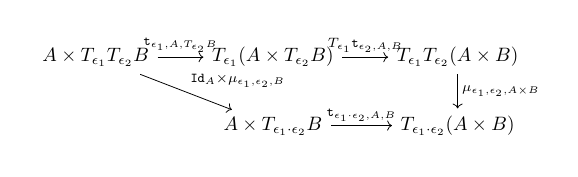
\begin{tikzpicture}[baseline= (a).base]
                \node[scale=.7] (a) at (0,0){
            \begin{tikzcd}[ampersand replacement=\&]
                A \times \T{\e_1}{\T{\e_2}{B}} 
                \arrow [r, "\tstrength{\e_1}{A}{\T{\e_2}{B}}"]
                \arrow [dr, "\Id{A} \times \bind{\e_1}{\e_2}{B}"]
                \& 
                \T{\e_1}{(A \times \T{\e_2}{B})} 
                \arrow [r, "\T{\e_1}{\tstrength{\e_2}{A}{B}}"]
                \& 
                \T{\e_1}{\T{\e_2}{(A \times B)}} 
                \arrow [d, "\bind{\e_1}{\e_2}{A \times B}"]
                \\
                \&
                A \times \T{\e_1 \dot \e_2}{B}  
                \arrow [r, "\tstrength{\e_1 \dot \e_2}{A}{B}"] 
                \&
                \T{\e_1 \dot \e_2}({A \times B)}
            \end{tikzcd}
            };
\end{tikzpicture}
            \caption{How the tensor strength natural transformation commutes with the join natural transformation.}
            \label{TensorStengthJoin}
        \end{minipage}
    
        \quad
        \begin{minipage}{0.45\textwidth}
            \begin{tikzcd}[ampersand replacement=\&]
                A \times B
                \arrow [r, "\Id{A} \times \point{B}"]
                \arrow [rd, "\point{A \times B}"]
                \&
                A \times \tob 
                \arrow [d, "\tstrength{\1}{A}{B}"]
                \\
                \&
                \T{\1}{(A \times B)}
            \end{tikzcd}
            \caption{How the tensor strength natural transformation commutes with the unit natural transformation}
            \label{TensorStrengthPoint}
        \end{minipage}
\end{framed}
\end{figure}



\begin{figure}
    \centering
    \begin{framed}
        \centering
            \begin{tikzcd}[ampersand replacement=\&]
                (A\times B)\times \T{\e}{C} 
                \arrow [rr, "\tstrength{\e}{(A\times B)}{C}"]
                \arrow [d, "\alpha_{A, B, \T{\e}{C}}"]
                \& \& \T{\e}{((A \times B)\times C)}
                \arrow [d, "\T{\e}{\alpha_{A, B, C}}"]
                \\
                A \times (B \times \T{\e}{C}) 
                \arrow [r, "\Id{A}\times\tstrength{\e}{B}{C}"]
                \&
                A\times\T{\e}{(B \times C)} 
                \arrow [r, "\tstrength{\e}{A}{(B \times C)}"]
                \& \T{\e}{(A \times (B \times C))}
                \\
            \end{tikzcd}
    \end{framed}
    \caption{Tensorial strength commutes with the reordering natural transformation.}
    \label{TensorStrengthAlpha}
\end{figure}






\subsection{Adjunction}\label{WhatsAnAdjunction}
An important concept in category theory is that of an Adjunction. Given functors $F: C\rightarrow D$, and  $G: D\rightarrow C$ and a pair natural transformations, known respectively as the unit and co-unit: $\eta_A: A \rightarrow G(F A)$ in $\C$ and $\epsilon_B: F(G B) \rightarrow B$ in $\DC$, such that $\epsilon_{F A}\after F(\eta_A) = \Id{F A}$ and $G(\epsilon_B)\after \eta_{F B} = \Id{G B}$ We can then use $\epsilon$ and $\eta$ to form a natural isomorphism between morphisms in the two categories, as seen in figure \ref{Adjunction}. This natural isomorphism is called an adjunction.


\begin{figure}
    \begin{framed}
    \begin{align*}
        \bar{(-)}: \quad\C(FA, B) &\leftrightarrow \DC(A, GB)   \quad: \widehat{(-)}\\
        f & \mapsto G(f)\after\eta_A \\
        \epsilon\after F(g) & \mapsfrom g\\
    \end{align*}
    \end{framed}
    \caption{How to construct the adjunction isomorphism from its unit and co-unit.}
    \label{Adjunction}
\end{figure}

\subsection{Strictly Indexed Category}

The final piece of category theory required to understand this dissertation is the concept of a strictly indexed category. A strictly indexed category is a functor from a \textit{base category} $\C$ into a target (\textit{indexed}) category of categories, where objects are categories and morphisms are functors. Objects, $A$, in the base category are mapped to categories $\C(A)$, known as \textit{fibres} in the indexed category. Morphisms between objects in the base category, $f: B\rightarrow A$, are contravariantly mapped to functors, written $f\star: \C(A)\rightarrow \C(B)$ and known as \textit{re-indexing functors}, between fibres in the indexed category. The strictly adverb indicates that the indexing in this construction is done by a functor as opposed to the weaker pseudofunctor (weak 2-functor) structure. Since pseudofunctors are not needed to explain anything in this project, I shall leave out their definition, though an interested reader may wish to research them further. \footnote{https://ncatlab.org/nlab/show/pseudofunctor}. 


Due to the composition laws for functors, $\theta\star\after\phi\star = (\phi\after\theta)\star$ and $\Id{A}*(B) = B\in\obj \C(A)$, and $\Id{}\star$ is the identity functor. For example, we may use the category of cartesian closed categories and cartesian closed functors, ($\cccat$) indexed by a partial-order, $\mathbb{P}$:

\begin{align*}
    I: \mathbb{P} & \rightarrow \cccat\qt{The indexing functor} \\
    A \in\obj\mathbb{P} & \mapsto \C \in\cccat\qt{Objects are mapped to categories}\\
    A \leq B & \mapsto (A \leq B)\star: \C \rightarrow \DC\qt{Morphisms are mapped to functors preserving CCC properties.}
\end{align*}

\section{Language Features and Their Requirements}\label{LanguageFeatureRequirements}


Different languages require different structures to be present in a category for the category to be able to interpret terms in the language. Using the concepts defined in section \ref{CategoryTheoryRequirements}, I shall now give an introduction to which category-theoretic structures are required to interpret different language features. 

One of the simplest, while still interesting, languages to derive a denotational semantics for is the simply typed lambda calculus (STLC). STLC's semantics require a cartesian closed category (CCC, see section \ref{CCC}).

Products in the CCC are used to denote the lists of variable types in the term environments, exponential objects model functions, and the terminal object is used to derive representations of ground terms, such as the unit term, $()$, as well as the empty term environments.

\begin{itemize}
    \item Products are used to construct type environments. $\deno{\G} = \deno{\nil, x: A, y:B, ... z:C} = \1 \times \deno{A} \times \deno{B} \times ... \times \deno{C}$
    \item Terminal objects are used in the denotation of constant terms $\deno{\gtyperelation{\const{A}}{A}} = \deno{\const{A}}\after\term{\deno{\G}}$
    \item Exponentials are used in the denotations of functions. $\deno{\typerelation{\G}{\lam{x}{A}{v}}{\ab}} = \cur{\deno{\typerelation{\gax}{v}{B}}}$
\end{itemize}

From this, we can specify what structures categories need to have in order to model more complex languages.
\begin{center}
    \begin{tabular}{|c|c|}
        \hline
        Language Feature & Structure Required \\
        \hline
        \hline
        STLC            & CCC \\
        \hline
        If expressions and booleans   & Co-product of the terminal object with itself and subtyping \\
        \hline
        Single Effect   & Strong Monad \\
        \hline
        Multiple Effects & Strong Graded Monad \\
        \hline
        Polymorphism & Indexed Category \\
        \hline
    \end{tabular}
\end{center}

To model if-expressions of the form $\pifthenelse{}{\texttt{condition}}{\texttt{if_true}}{\texttt{if_false}}$, we need a way to combine morphisms of the form $\deno{\gtyperelation{\texttt{condition}}{\B}}: \G\rightarrow\deno{\B}$, $\deno{\gtyperelation{\texttt{if_true}}{A}}: \G\rightarrow A$, and $\deno{\gtyperelation{\texttt{if_false}}{A}}: \G\rightarrow A$ to form a morphism $\G\rightarrow A$. If we have a co-product $\G + \G$, and a morphism mapping $\B$s to $\G + \G$, we could use the fold morphism $[\deno{\texttt{if_true}}, \deno{\texttt{if_false}}]$ to achieve the required . It turns out that using exponentials, as seen in the denotation of the (If) type rule in figure \ref{TermDenotations}, we can factor out the $\G$ to instead use a co-product  $\1 + \1$ instead of $\G + \G$. It now a natural choice to use $\1 + \1$ as $\deno{\B}$. Hence we can model the boolean values $\t, \f$ as the co-product constructors $\inl, \inr$.

A single effect can be modelled by adding a strong monad to the category, as shown by Moggi \cite{MoggiMonads}. A language with an explicit monad in its type system requires two operations: \textit{return} and \textit{bind}, the type rules for which can be seen in equation \ref{MonadTypeRules}. The $\M{}{(-)}$ type constructor represents values which have an instance of the effect associated with their computation. The \textit{return} operator lifts pure values (with no associated effects) into the effectful type constructor. The \textit{bind} operator (often supplemented with some \texttt{do .. in ...} syntax) allows us to compose together expressions which have effects. As shown by Moggi \cite{MoggiMonads}, these two operations can be modelled using the \textit{unit} and \textit{join} natural transformations of a strong graded monad. The monad needs to be strong in order to allow access to variables in the environment from within the monadic expression. An example of this can be seen in figure \ref{MonadStrengthRequirement}. 

\begin{figure}
    \begin{framed}
        \textbf{Motivating the Tensor Strength Requirement}
        \begin{framed}
            \begin{lstlisting}[
                mathescape,
                columns=fullflexible,
                basicstyle=\fontfamily{lmvtt}\selectfont,
              ]
let $x$ = $5$ in (
    do $y$ $\texttt{<-}$ readInt in (
        return $x$ + $y$
    ) 
);
            \end{lstlisting}
        \end{framed}
        
In the \texttt{return} clause, the program makes reference to variables $x$ and $y$ from the environment. Since $x$ is defined inside the monadic \texttt{do} clause, it is not available to clauses in the body of the clause without a means to convert the type $(\G \times \M{}{A)}$ to $\M{}{(\G\times A)}$.
\end{framed}
   
\caption{Program in a monadic effectful language that requires tensor strength of the effect's monad to execute.}
\label{MonadStrengthRequirement}
\end{figure}

\begin{eqnarray}\label{MonadTypeRules}
    \ntreeruleI{Return}{\typerelation{\G}{v}{A}}{\typerelation{\G}{\return{v}}{\M{}{A}}} & \ntreeruleII{Bind}{\typerelation{\G}{v_1}{\M{}{A}}}{\typerelation{\gax}{v_2}{\M{}{B}}}{\typerelation{\G}{\doin{x}{v_1}{v_2}}{\M{}{B}}}
\end{eqnarray}

For a more precise analysis of languages with multiple effects, we can look into whether there is an algebra on the effects. For example, we might want to express what the composite effect of two sequential expressions with different effects. We could follow an expression that might throw an exception with one that accesses mutable state and a third that carries out IO transactions. We would also want some form of \textit{unit} effect for pure expressions which does nothing when composed with other effects. Finally, to make it easier to analyse branched code, such as \textit{if expressions}, some form of subtyping would be useful. This structure is modelled exactly by an appropriate partially-ordered monoidal algebra $(E, \dot, \subeffect, \1)$. The set $E$ gives the various effects that can be produced, $\1$ represents the unit effect for pure values, $\dot$ allows us to associatively compose multiple effects and the partial-order  $\subeffect$ gives us a subtyping of effects for an intuitive if-statement programming model.

In order to embed this algebra-based effect analysis in the type system, we can index Moggi's monadic type constructor $\M{}{}$ with the effect $\e$ that is produced when the corresponding expression is evaluated. Further more, when we use the \textit{return} operation to lift pure values into the monadic type constructor, the resulting monadic type should have an index of $\1$ indicating that the effect produced is pure. Finally, when we \textit{bind} together effectful expressions, the resulting effect should be the composition of the effects of the subexpressions. Putting together these requirements yields the new type rules given in equation \ref{GradedMonadTypeRules}. By suitably extending the monad laws to account for this new indexing, we find that we require a strong graded monad to model these features using category theory. This construct was first documented in the context of semantics by Katsumata (\cite{Katsumata:2014}).

\begin{eqnarray}\label{GradedMonadTypeRules}
    \ntreeruleI{Return}{\typerelation{\G}{v}{A}}{\typerelation{\G}{\return{v}}{\moa}} & \ntreeruleII{Bind}{\typerelation{\G}{v_1}{\M{\e_1}{A}}}{\typerelation{\gax}{v_2}{\M{\e_2}{B}}}{\typerelation{\G}{\doin{x}{v_1}{v_2}}{\M{\e_1 \dot \e_2}{B}}}
\end{eqnarray}


When we combine an effect system with if-expressions, we come across another, language-level, issue. When programming using the construct, we might want the true and false branches of the expressions to have different effects. For example, one branch of an expression may perform I/O operations, whilst the other has no side effects. Since effect analysis is done by the type system, this means that the two branches have different types. Hence the typical type rule  for if-expressions, as given in equation \ref{IfTypeRule}, does not hold. A solution for this is to introduce a notion of subtyping. If $\gtyperelation{v}{A}$ and $A \subtype B$, then $\gtyperelation{v}{B}$. Using the partial-order on effects to generate the subtyping relation, we can now unify compatible, though not equal, effects in an if-expression.

\begin{equation}\label{IfTypeRule}
    \ntreeruleIII{If}{
        \gtyperelation{\texttt{condition}}{\B}
    }{
        \gtyperelation{\texttt{if_true}}{A}
    }{
        \gtyperelation{\texttt{if_false}}{A}
    }{
        \gtyperelation{
            \pifthenelse{}{
                \texttt{condition}
            }{
                \texttt{if_true}
            }{
                \texttt{if_false}
            }
        }{A}
    }
\end{equation}

To model sub-typing, we need a way to convert morphisms $\deno{\gtyperelation{v}{A}}: \G\rightarrow A$ to $\deno{\gtyperelation{v}{B}}:\G\rightarrow B$ when $A\subtype B$. This can be done if for each instance of $A\subtype B$, we have a there is morphism $\deno{A\subtype B}: A \rightarrow B$. These morphisms should respect the antisymmetry, transitivity, and reflexivity of the subtyping relation, meaning that $\deno{B\subtype C}\after\deno{A\subtype B} = \deno{A\subtype C}$ and $\deno{A\subtype A} = \Id{A}$.

Polymorphism is a harder concept to explain intuitively. The particular flavour of polymorphism that this dissertation discusses is System-F-Style parametric polymorphism. For a given type-system feature $F$, such as types, effects, type constructors, or some other language specific feature, we can add parametric polymorphism over $F$ by allowing instances of $F$ to be replaced by $F$ variables and introducing certain type expressions to modify the types. For example, let us look at system F \cite{SystemFIntroduction}. System F has polymorphism over types. This means that we can replace a type expression with a type variable parameter. We also need to be able to syntactically generalise over type parameters and to be able to specify a particular type parameter's value. This requires us to extend the syntax of the simply typed lambda calculus with the appropriate specialisation and generalisation terms as well as parameterised types, as seen in figure \ref{SystemFTermsTypes}.

\begin{figure}
    \begin{framed}
        \centering
        \textbf{System F}

        Types are extended with variables and parameterisation terms.
        \begin{align*}
            A \gens ... \mid \a\mid \all{\a}{A}
        \end{align*}

        Values are extended with generalisation and specialisation terms respectively.
        \begin{align*}
            t \gens ... \mid \elam{\a}{t}\mid \eapp{t}{A}
        \end{align*}
    \end{framed}
    \caption{The extensions made to the simply typed lambda calculus which yield System F}
    \label{SystemFTermsTypes}
\end{figure}

To correctly account for these new terms and types in the type system, we need to ensure that all parameterisations are soundly constructed, in a similar way to how a closed term in the simply typed lambda calculus has no free variables. To do this, we introduce a new $F$-environment $\P$ to complement the term environments $\G$. A term or type is well formed (written $\wellformed{\P}{f}$) only if it only contains $F$ variables in $\P$. An $F$ expression, $f$, is also well formed only if it only contains $F$ variables in $\P$. We can now specify type rules for the generalisation (parameterisation of an expression over an $F$-variable) and specialisation (substituting a parameter for a value) of terms. As seen in equation \ref{PolymorphismTypeRules}.

\begin{eqnarray}\label{PolymorphismTypeRules}
    \ntreeruleI{Gen}{\etyperelation{\P, \a}{\G}{v}{A}}{\gpetyperelation{\elam{\a}{v}}{\all{\a}{A}}}& 
    \ntreeruleII{Spec}{\gpetyperelation{v}{\all{\a}{A}}}{\wellformed{\P}{f}}{\gpetyperelation{\eapp{v}{f}}{A\ssub{\a}{f}}}
\end{eqnarray}

If we can model the language without the polymorphic terms, with each specific $F$ environment, then we can instantiate a collection of categories, each of which models the language at a given $F$ environment. This collection of categories (or fibres) can be indexed by a base category, the structure of which models the $F$ environments and relationships between them. We can hence construct an indexed category, whereby each $F$ environment in the base category is mapped to the fibre modelling the semantics at the specific environment, and morphisms between $F$ environments correspond to functors between the respective fibres. Figure \ref{IndexDiagram} demonstrates this construction. If we model an $F$ environment $\P, \a$ as a product, then the $\p$ morphism represents removing $\a$ from the environment and the $\pstar$ functor conversely increases the size of the environment. As will be show later in this dissertation, if $\pstar$ has a right adjoint (see section \ref{WhatsAnAdjunction}), $\forall$, then this adjunction can be used to model generalisation and specialisation of polymorphic terms. This will be explained in the next chapter. 

How the fibres are derived from objects in the base category depends on the polymorphic properties of the language being modelled. For example, in system F, types are impredicative. That is, types can quantify over any other types, including themselves. This means that there has to be a strong coupling between the base category, which represents type-variable environments and transformations upon them and objects in the fibres, which represent types. This typically manifests in the set of objects  in each fibre being in bijection with the set of morphisms from the appropriate type-variable environment in the base category. Since, in effect-polymorphic languages, types quantify over effects, but effects do not quantify over themselves, we can conceptually decouple the objects in the fibres from the base category, meaning that effect-polymorphic models are simpler to define. 

In this dissertation, I show how these category theoretic building blocks can be put together to give the class of categories that can model polymorphic effect systems.

\begin{figure}[ht!]
    \scalebox{0.9}{
        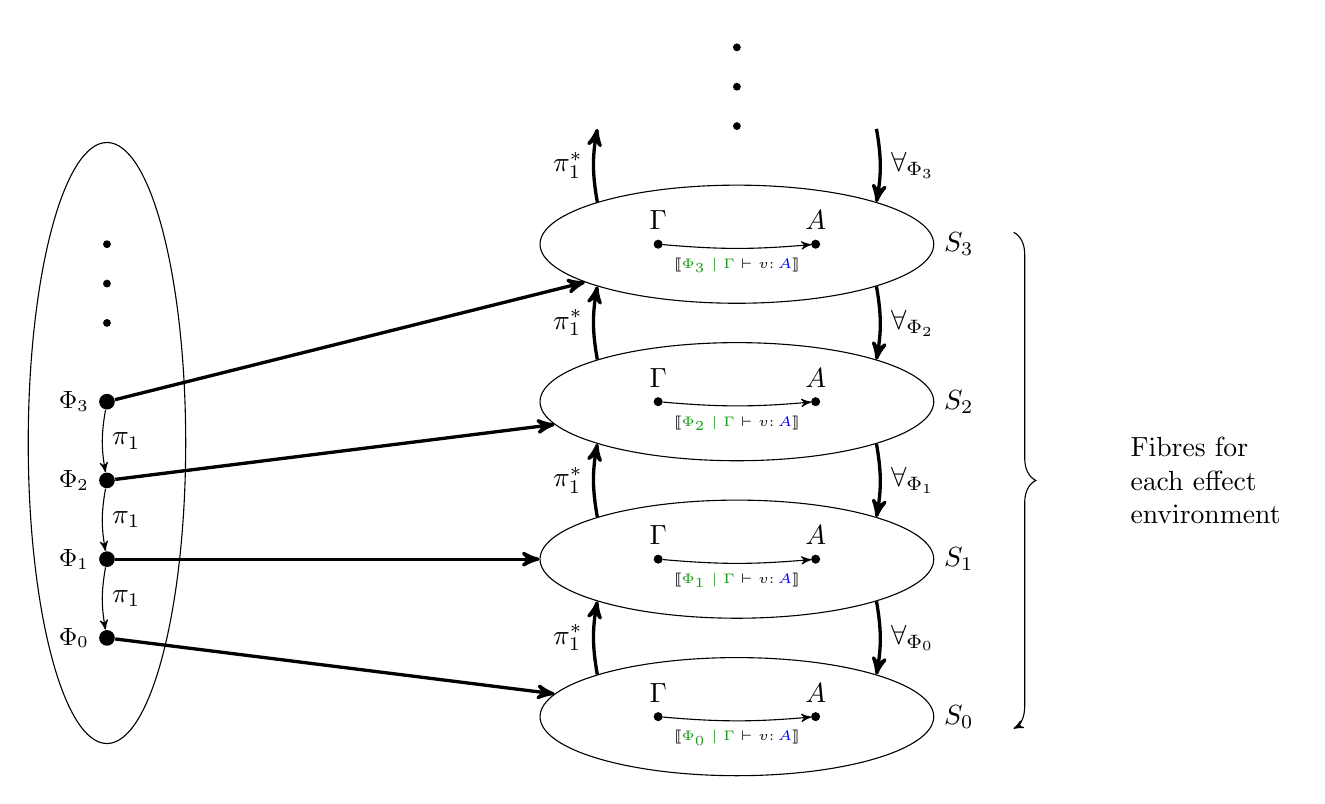
\begin{tikzpicture}[->,>=stealth']]
            % Draw the env objects
            \foreach \y[count=\c,evaluate={\yi=int(\c-1)}] in {3, 4, 5, 6}{
                \node[fill,circle,inner sep=2pt,label=left:{\small $\P_\yi$}] (d\yi) at (0,\y) {};
            }
    
            % draw the ... above the env objects
            \foreach \y[count=\c,evaluate={\yi=int(\c-1)}] in {7, 7.5, 8}{
                \node[fill, circle, inner sep=1pt] (dd\yi) at (0,\y){};
            }
            % Draw the index category
            \node[fit=(d0) (d1) (d2) (d3) (dd0) (dd1) (dd2),ellipse,draw,minimum width=2cm] {};
    
            %draw the s-category stack
            \foreach \y[count=\c,evaluate={\yi=int(\c-1)}] in {2, 4, 6, 8}{
                \node[circle, draw, inner sep=1pt, fill, label=above:{$\G$}] (g\yi) at (7,\y){};
                \node[circle, draw, inner sep=1pt, fill, label=above:{$A$}] (a\yi) at (9,\y){};
                \draw[->](g\yi) to[bend right=5] node[below]{\tiny $\deno{\etyperelation{\P_\yi}{\G}{v}{A}}$} (a\yi);
                \node[ellipse, draw, minimum width=5cm, minimum height=15mm,label=right:$S_\yi$] (s\yi) at (8,\y){};
            }
    
            % Hidden ellipse to draw functors to
            \node[ellipse, minimum width=5cm, minimum height=15mm] (s4) at (8,10){};
    
            %Draw the ... for the s-category stack
            \foreach \y[count=\c,evaluate={\yi=int(\c-1)}] in {9.5, 10, 10.5}{
                \node[fill, circle, inner sep=1pt] (p\yi) at (8, \y){};
            }
    
            % Draw index arrows
            \foreach \i in {0, 1, 2, 3}{
                \draw[->, very thick] (d\i) to (s\i);
            }
    
            % draw the re-indexing functors
    
            \foreach \source[count=\dest] in {0, 1, 2, 3}{
                \draw[->, very thick](s\source.north west) to[bend left=10] node[left]{$\pstar$} (s\dest.south west);
            }
    
            % Draw the quantification functors
            \foreach \dest[count=\source] in {0, 1, 2, 3}{
                \draw[->, very thick] 
                (s\source.south east) to[bend left=10] node[right]{$\forall_{\P_\dest}$} (s\dest.north east);
            }
    
            % Draw the internal morphisms in base category
            \foreach \dest[count=\source] in {0, 1, 2}{
                \draw[->]
                (d\source) to[bend right=10] node[right]{$\p$} (d\dest);
            }
    
            %Draw the bracket
    
            \draw [decoration={brace,amplitude=8pt},decorate] ($(s3)+(10em,1ex)$) -- ($(s0)+(10em,-1ex)$);
            \node[text width=20mm] (Label) at (14,5){Fibres for each effect environment};
        \end{tikzpicture}
    }
    
    \caption{Diagram of the structure of an indexed category for modelling a polymorphic language. Thick arrows between categories represent functors and finer arrows withing categories represent internal morphisms. The left hand category is the base category.
    }
    \label{IndexDiagram}
\end{figure}


\section{The Effect Calculus}

The basic effect calculus is an extension of the simply typed lambda calculus to include constants, \texttt{if} expressions, effects, and subtyping. It has terms of the following form:

\begin{align*}
    v ::= \const{A} \mid x\mid \t \mid\f \mid\u\mid\lam{x}{A}{v}\mid\apply{v_1}{v_2}\mid\return{v}\mid\doin{x}{v_1}{v_2}\mid\pifthenelse{A}{v}{v_1}{v_2} 
\end{align*}

Where $\const{A}$ is one of collection of ground constants, and $A$ ranges over the types:

\begin{align*}
    A, B, C ::= \g\mid \ab \mid\mea
\end{align*}

Where $\g$ is from a collection of ground types, including $\U, \B$, and $\e$ ranges over partially-ordered monoid of effects: $(E, \dot, \subeffect, \1)$.

The calculus has a simple, Haskell style semantics. Lambda terms when applied to a parameter substitute their bound variable for the parameter expression, as seen in figure \ref{ECBeta}, if statements pick a branch once their condition is decided to be true or false, figure \ref{ECIf}, and finally the monadic effects behave in a similar way to Haskell's monad type class. It is difficult to simply formalise an operational $\beta\eta$-reduction semantics for a monadic language without a concrete instantiation of the graded monad. Instead, the monad should obey the equational laws given in figure \ref{ECMonads}.


\begin{figure}
    \begin{framed}
        \begin{align*}
            \apply{(\lam{x}{A}{v_1})}{v_2} & \rightsquigarrow v_1\ssub{x}{v_1}
        \end{align*}
    \end{framed}
    \caption{The $\beta$ reduction lambda terms of lambda terms in the effect calculus.}
    \label{ECBeta}
\end{figure}

\begin{figure}
    \begin{framed}
        \begin{align*}
            \pifthenelse{A}{\t}{v_1}{v_2} & \rightsquigarrow v_1\\
            \pifthenelse{A}{\t}{v_2}{v_2} & \rightsquigarrow v_2\\
        \end{align*}
    \end{framed}
    \caption{The reduction of if expressions in the effect calculus.}
    \label{ECIf}
\end{figure}


\begin{figure}
    \begin{framed}
        \begin{align*}
            \doin{x}{\return{v_1}}{v_2} & \rightsquigarrow v_2\ssub{x}{v_1}\\
            \doin{x}{v}{\return{x}} & \rightsquigarrow v\\
            \doin{x}{v_1}{(\doin{y}{v_2}{v_3})} 
            & \leftrightsquigarrow\quad  \doin{y}{(\doin{y}{v_1}{v_2})}{v_3}
        \end{align*}
    \end{framed}
    \caption{The monad laws for the effect calculus.}
    \label{ECMonads}
\end{figure}



As an example, by instantiating the language with the appropriate constants, ground effects, and ground types, we can write the programs in figure \ref{CheckExample}.

\begin{figure}
    \centering
    \begin{minipage}{0.45\textwidth}
        \begin{framed}
            \begin{lstlisting}[
                mathescape,
                columns=fullflexible,
                basicstyle=\fontfamily{lmvtt}\selectfont,
              ]
do $b$ $\texttt{<-}$ Prompt("Are You Sure?") in (
    if $b$ then
        FireMissiles
    else
        AbortMissiles
)
            \end{lstlisting}        
        \end{framed}
    \end{minipage}
    \quad
    \begin{minipage}{0.45\textwidth}
        \begin{framed}
            \begin{lstlisting}[
                mathescape,
                columns=fullflexible,
                basicstyle=\fontfamily{lmvtt}\selectfont,
              ]
$\lambda$ $alice$: Agent. (
    $\lambda$ $bob$: Agent. (
    do $amount$ $\texttt{<-}$ AwaitPayment($alice$)
    in SendPayment($bob$, $amount$)
    )
)
              \end{lstlisting}
        \end{framed}
    \end{minipage}
    \caption{A pair of examples of non-polymorphic programs}
    \label{CheckExample}
\end{figure}



Already, we can see where having effect polymorphism in the language would be useful. We could make the first example in figure \ref{CheckExample} into a more general procedure that prompts a user to confirm any I-O action, as can be seen in the extended example in figure \ref{PolymorphicCheckExample}.

\begin{figure}
\begin{framed}
    \begin{lstlisting}[
        mathescape,
        columns=fullflexible,
        basicstyle=\fontfamily{lmvtt}\selectfont,
      ]
$\Lambda$ $Action$: Effect. 
$\lambda$ $ifConfirmed$: $Action$.
$\lambda$ $ifAborted$: $Action$.
do $b$ $\texttt{<-}$ Prompt("Are You Sure?") in (
    if $b$ then 
        $ifConfirmed$ 
    else
        $ifAborted$
)
    \end{lstlisting}        
\end{framed}
\caption{A polymorphic version of the checking example}
\label{PolymorphicCheckExample}
\end{figure}


\section{Polymorphic Effect Calculus}

Next, we consider the Effect Calculus extended with terms to allow System-F-style polymorphism over effects.

\begin{align*}
    v::=\text{..}\mid\elam{\a}{v}\mid\eapp{v}{\e}
\end{align*}

\begin{align*}
    A, B, C::=\text{...}\mid \all{\a}{A}
\end{align*}

\begin{align*}
    \e ::= e \mid \a \mid \e\dot\e
\end{align*}

Where effects $\e$ now range over the effect partially-ordered monoid augmented with effect variables from an environment $\P = \nil, \a, \b ...$ (where $\nil$ represents the empty list), written as $(E_\P, \dotp, \subeffectp, \1)$. The ground effects of $E$ are now ranged over by $e$ and $\e$ ranges over effects including effect variables. The operator $\dotp$ is the extension of the original $\dot$ operator to symbolically act on expressions including effect variables. For example, if for some $\e$, $\forall \e'. \e'\dot\e = \e'$ then $\a\dotp\e = \a$ for some appropriate effect-variable environment $\P$.




\subsection{Type System}
\subsubsection{Environments}
As mentioned before, effects can now include effect variables. These are managed in the type system using a well-formed effect-variable environment $\P$, which is a snoc-list.

\begin{align*}
    \P ::= \nil \mid \P, \a
\end{align*}



\subsubsection{Effects}
The ground effects form the same monotonic, partially-ordered monoid $(E, \dot, \1, \subeffect)$ over ground elements $e$. For each effect environment $\P$, we define a new, symbolic partially-ordered monoid:

\begin{equation}
    (E_\P, \dotp, \1, \subeffectp)
\end{equation}

Where $E_\P$ is the closure of $E\cup \left\{\a\mid\a\in\P\right\}$ under $\dotp$, which is defined as:

\begin{equation}
    \treeruleI{\e_3 = \e_1\dot\e_2}{\e_3 = \e_1\dotp\e_2}
\end{equation} 

For variable-free terms and is defined symbolically for variable-containing terms. Further more, we also define the subeffecting relation in terms of its variables and the ground relation.

\begin{equation}
    \e_1 \subeffectp \e_2 \Leftrightarrow \forall \si\downarrow. \e_1\sub{\si\downarrow} \subeffect \e_2\sub{\si\downarrow}
\end{equation}

Where $\si\downarrow$ denotes any ground-effect substitution of $\P$. That is any substitution of all effect variables in $\P$ to ground effects. Where it is obvious from the context, I shall use $\subeffect$ instead of $\subeffectp$.


\subsubsection{Types}
As stated, types are now generated by the following grammar.

$$ A, B, C \gens \ground \mid \ab \mid \mea \mid \all{\a}{A}$$
  
\subsubsection{Type Environments}
As is often the case in similar type systems, a type environment is a snoc list of term-variable, type pairs, $\G \gens \nil \mid \gax$.

\paragraph{Domain Function on Type Environments}

\[
    \dom{\nil} = \emptyset
    \quad\quad\quad
    \dom{\gax} =  \dom{\G}  \cup \left\{x \right\}
\]

\subsubsection{Well-Formedness Predicates}
To formalise properties of the type system, it will be useful to have a collection of predicates ensuring that structures in the language are well behaved with respect to their use of effect variables.

Informally, $\a \in \P$ if $\a$ appears in the list represented by $\P$.

The $\ok{}$ predicate on effect environments asserts that the effect environment does not contain any duplicated effect variables.

\[
    \ntreerulez{Nil}{\ok{\nil}}
\quad
    \condtreeruleI{Extend}{\ok{\P}}{\ok{\P, \a}}{\a\notin \P}
\]

Using this, we can define the well-formedness relation on effects, $\wellformed{\P}{\e}$. In short, this relation ensures that effects do not reference variables that are not in the effect environment. This is equivalent to saying that $\wellformed{\P}{\e}$ means that $\e\in E_\P$.

\[
    \ntreeruleI{Ground}{\ok{\P}}{\wellformed{\P}{e}}
    \quad
    \ntreeruleI{Var}{\ok{\P,\a}}{\wellformed{\P,\a}{\a}}
    \quad
    \condtreeruleI{Weaken}{\wellformed{\P}{\a}}{\wellformed{\P,\b}{\a}}{\a\neq\b, \b\notin\P}
    \quad
    \ntreeruleII{Compose}{\wellformed{\P}{\e_1}}{\wellformed{\P}{\e_2}}{\wellformed{\P}{\e_1\dot\e_2}}
\]

The well-formedness of effects can be used to a similar well-typed-relation on types, $\wellformed{\P}{A}$, which asserts that all effects in the type are well formed.

\[
    \ntreeruleI{Ground}{\ok{\P}}{\wellformed{\P}{\g}}
    \quad
    \ntreeruleII{Fn}{\wellformed{\P}{A}}{\wellformed{\P}{B}}{\wellformed{\P}{\ab}}
    \quad
    \ntreeruleII{Effect}{\wellformed{\P}{A}}{\wellformed{\P}{\e}}{\wellformed{\P}{\mea}}
    \quad
    \ntreeruleI{Quantification}{\wellformed{\P,\a}{A}}{\wellformed{\P}{\all{\a}{A}}}
\]

Finally, we can derive the a well-formedness of type environments,   $\oke{\P}{\G}$, which ensures that all types in the environment are well formed.

\[
    \ntreerulez{Nil}{\oke{\P}{\nil}}
    \quad
    \condtreeruleI{Extend}{\oke{\P}{\G}\s\s \wellformed{\P}{A}}{\oke{\P}{\gax}}{x\notin\dom{\G}}
\]

\subsubsection{Subtyping}

We assume that the set of ground types with a subtyping partial-order relation $\subtype_{\ground}$. This subtyping relationship could be the trivial partial-order, which only includes $A\subtypeg B$ if $A = B$, or could be a more interesting relation. As this relationship is a partial-order, it is antisymmetric, transitive and reflexive.
    \[
        \ntreerulez{Reflexive}{A \subtype_{\ground} A}
        \quad
        \ntreeruleII{Transitive}{A \subtype_{\ground} B}{B \subtype_{\ground} C}{A \subtype_{\ground} C}
    \]

Using this ground type relation, we can then construct a subtyping relation between pairs of types $A, B$ with respect to an effect environment $\P$.

\[
    \scalebox{0.85}{$
    \ntreeruleI{Ground}{A \subtype_{\ground} B}{A \subtypep B}
    \quad
    \ntreeruleII{Fn}{A \subtypep A'}{B' \subtypep B }{\fntype{A'}{B'} \subtypep \ab}
    \quad
    \condtreeruleI{Quantification}{A\subtypep A'}{\all{\a}{A}\subtypepa\all{\a}{A'}}{\a\notin\P}
    \quad
    \ntreeruleII{Effect}{A\subtypep B}{ \e_1\subeffectp\e_2}{\M{\e_1}{A}\subtypep\M{\e_2}{B}}
    $}
\]

Since the ground subtyping and subeffecting relations are partial-order, it is fairly simple to prove by induction that the new relation is also a partial-order. By induction, it is also easy to prove that if $A \subtypep B$ and $\wellformed{\P}{A}$ then $\wellformed{\P}{B}$. This last property comes about because the labelled subeffecting relation $\subeffectp$ only holds between effects in $E_\P$.


\subsubsection{Type Rules}
We define a fairly standard set of type rules on the language.

\[
    \scalebox{0.85}{$
    \ntreeruleII{Const}{\oke{\P}{\G}}{\wellformed{\P}{A}}{\gpetyperelation{\const{A}}{A}} 
    \quad
    \ntreeruleI{Unit}{\oke{\P}{\G}}{\gpetyperelation{\u}{\U}} 
    \quad
    \ntreeruleI{True}{\oke{\P}{\G}}{\gpetyperelation{\t}{\B}}
    \quad
    \ntreeruleI{False}{\oke{\P}{\G}}{\gpetyperelation{\f}{\B}}
    $}
\]
\[
    \scalebox{0.85}{$
\ntreeruleI{Var}{\oke{\P}{\gax}}{\etyperelation{\P}{\gax}{x}{A}}
\quad
\condtreeruleII{Weaken}{\etyperelation{\P}{\G}{x}{A}}{\wellformed{\P}{B}}{\etyperelation{\P}{\gby}{x}{A}}{x \neq y, y\notin\dom{\G}}
\quad
\ntreeruleI{Fn}{\etyperelation{\P}{\gax}{v}{B}}{\etyperelation{\P}{\G}{\lam{x}{A}{v}}{\ab}}
$}
\]
\[
    \scalebox{0.85}{$
    \ntreeruleII{Subtype}{\etyperelation{\P}{\G}{v}{A}}{A \subtypep B}{\etyperelation{\P}{\G}{v}{B}}
    \quad
    \ntreeruleI{Effect-Gen}{\etyperelation{\P,\a}{\G}{v}{A}}{\gpetyperelation{\elam{\a}{v}}{\all{\a}{A}}}
    \quad
    \ntreeruleII{Effect-Spec}{\gpetyperelation{v}{\all{\a}A}}{\wellformed{\P}{\e}}{\gpetyperelation{\eapp{v}{\e}}{A\ssub{\a}{\e}}}
    $}
\]
\[
    \scalebox{0.85}{$
    \ntreeruleI{Return}{\gpetyperelation{v}{A}}{\gpetyperelation{\return{v}}{\moa}}
    \quad
    \ntreeruleII{Apply}{\gpetyperelation{v_1}{\ab}}{\gpetyperelation{v_2}{A}}{\gpetyperelation{\apply{v_1}{v_2}}{B}}
    $}
\]
\[
    \scalebox{0.85}{$
    \ntreeruleIII{If}{\gpetyperelation{v}{\B} }{ \gpetyperelation{v_1}{A}}{\gpetyperelation{v_2}{A}}{\gpetyperelation{\pifthenelse{A}{V}{v_1}{v_2}}{A}}
    \quad
    \ntreeruleII{Bind}{\gpetyperelation{v_1}{\M{\e_1}{A}}}{\etyperelation{\P}{\gax}{v_2}{\M{\e_2}{B}}}{\gpetyperelation{\doin{x}{v_1}{v_2}}{\M{\e_1 \dot \e_2}{B}}}
    $}
\]

\subsubsection{Ok Lemmas}

\begin{lemma}[Ok Lemma on Type Environments]
    The first lemma used in this dissertation is: if $\gpetyperelation{v}{A}$ then $\oke{\P}{\G}$.
\end{lemma}
\begin{proof}
    If $\oke{\P}{\gax}$ then by the inversion (See figure \ref{InversionPrinciple}) of the $\ok{}$ rule, we have $\oke{\P}{\G}$ 

    Only the type rule \textit{(Weaken)} adds terms to the environment from its preconditions to its postcondition and it does so in an $\ok{}$ preserving way. Any type derivation tree has at least one leaf. All leaves are axioms which require $\oke{\P}{\G}$. And all non-axiom derivations preserve the $\ok{}$ property.
    $$\square$$
\end{proof}

\begin{lemma}[Ok Lemma on Effect Environments]
    A second group of lemmas is that each of the judgments  $\wellformed{\P}{\e}$, $\wellformed{\P}{A}$, and $\oke{\P}{\G}$ implies $\ok{\P}$.
\end{lemma}

\begin{proof}
    We shall prove each of the implications separately, but an over-arching theme of this proof is that the leaf rules of any $\wellformed{\P}{\texttt{Consequence}}$ derivation tree require $\ok{\P}$ and that any modifications to the effect environment in the assumptions to the effect environment in the consequence of a rule preserve the $\ok{}$ relation. Hence, using induction and inversion, we can show that the effect environment is always well formed in any complete derivation tree.

    Firstly in the case of the well-formedness relation $\wellformed{\P}{\e}$, the only leaf rules are the (\textit{Ground}) and (\textit{Var}) rules. By inversion, if $\wellformed{\P}{e}$ or $\wellformed{\P, \a}{\a}$ then $\ok{\P}$ or $\ok{\P, \a}$ respectively. Next, by inversion on the (\textit{Compose}) rule, if $\wellformed{\P}{\e_1\dot\e_2}$ then $\wellformed{\P}{\e_1}$, so by induction $\ok{\P}$. Finally, the weakening rule preserves the $\ok{}$ property of the effect environment, so $\wellformed{\P, \b}{\a} \implies \wellformed{\P}{\a} \implies \ok{\P} \implies \ok{(\P, \b)}$.

    Secondly, in the case of the well formedness relation on types, the only leaf rule is (\textit{Ground}). If $\wellformed{\P}{\g}$, then by inversion, $\ok{\P}$. Similarly to the (\textit{Compose}) rule for effects, the (\textit{Fn}) rule's preconditions have the same effect-environment, so $\ok{\P}$ holds by inversion and induction. By inversion on the (\textit{Effect}) rule, $\wellformed{\P}{\e}$ so $\ok{\P}$. Finally the (\textit{Quantification}) rule preserves $\ok{}$ in a similar way to the (\textit{Weaken}) rule above.

    Finally, if $\oke{\P}{\gax}$ then, by inversion, $\wellformed{\P}{A}$  and $\oke{\P}{\G}$. Since $\G$ is finite, $\oke{\P}{\nil}$. By inversion of the \textit{(Nil)} rule, $\ok{\P}$.
\end{proof}



\begin{figure}
    \begin{framed}
        \textbf{Inversion in Inductive Proofs}

        In proofs involving assumptions with multiple inductive rules, a useful property is that of inversion. This allows us to case split over the inductive rule that generated the assumption and can allow us to infer the structure of the term.

        For example, consider a theorem which assumes $\gpetyperelation{v}{B}$, then we can case split over the type rules. If $\gpetyperelation{v}{B}$ was generated by the (Apply) rule (\ref{InversionExample}), then by inspecting the rule, we can infer that there exist two subterms $\gpetyperelation{v_1}{\ab}$, $\gpetyperelation{v_2}{A}$ such that $v = \apply{v_1}{v_2}$. 

        \begin{equation}\label{InversionExample}
            \ntreeruleII{Apply}{\gpetyperelation{v_1}{\ab}}{\gpetyperelation{v_2}{A}}{\gpetyperelation{\apply{v_1}{v_2}}{B}}
        \end{equation}
        Then we might use the inferred subexpressions $v_1, v_2$ to prove the theorem in this case.
    \end{framed}
    \caption{An explanation of the concept of inversion.}
    \label{InversionPrinciple}
\end{figure}


\chapter{The Semantics of PEC in an Strictly Indexed Category}

In this chapter, I  describe the category structure required to interpret an instance of the PEC. I then present denotations of each type of structure in the language, such as types, effects, terms, substitutions, and environment weakenings. Finally, I provide outlines and interesting cases of the proofs of the lemmas leading up to and including soundness of the semantics with respect to a $\beta\eta$-conversion-based equational equivalence. However, firstly I shall give a brief treatment to the semantics of EC.


\section{Semantics for EC in an S-Category}\label{SCategoryIntro}

As suggested in section \ref{LanguageFeatureRequirements}, since EC contains multiple effects, STLC terms, and \texttt{if} expressions, we should be able to interpret its semantics in a cartesian closed category with an appropriate strong graded monad and the co-product $\1 + \1$. With the addition of some extra category structure to handle subtyping, which I shall explain shortly, it is indeed possible to interpret EC. This section contains a fairly high-level treatment of the semantics. This is because the concepts introduced are a subset of those required for the semantics of PEC, which I shall explain in more detail later. Semantics for similar languages to EC have been given using an S-category-style construct, such as by Katsumata \cite{Katsumata:2014}.


\begin{framed}
    \begin{definition}[S-Category]
        In order to correctly model a given instantiation of EC, that is an EC with a collection of effects, constants, and ground types, there should be a collection of objects in the category to represent the ground types. There should also be a point morphism (a morphism from the terminal object to the appropriate type) for each constant. In addition to the previously stated requirements, we also require an S-category, $\C$, to be able to model subtyping and subeffecting. For each instance of the ground subtyping relation, $A \subtypeg B$, there should exist a morphism between the objects representing the ground types $A$ and $B$. A further requirement is that $\C$ has a collection of subeffecting natural transformations. For each instance of $\e_1 \subeffect \e_2$, there exists a natural transformation $\db{\e_1\subeffect\e_2}: \T{\e_1}{}\rightarrow\T{\e_2}{}$ such that it has interactions with the graded monad as specified in figures \ref{SubeffectTensorStrength}, \ref{SubeffectBind}. We can now define morphisms for all forms of subtyping by constructions following the derivation tree for subtyping. For more detail, one can look at section \ref{PECDenotations} and below for the same construction on PEC. From this point onwards, I shall refer to a category that fulfills these properties of having a strong graded monad, CCC, ground objects and points, subeffect natural transformations, and a co-product $\1 + \1$ as an \textit{S-Category} (Semantic Category).
    \end{definition}
\end{framed}

A full derivation and proof of soundness of the semantics of the Effect Calculus can be found online on my github repository \footnote{\todo{Correct Link}} as it is too long to include here and many of the concepts are repeated later in the remainder of this dissertation anyway. The categorical semantics of the Effect Calculus requires an S-category not only to simply model all of the features of EC but also to use the various commutivity diagrams and rules to manipulate the expressions encountered when proving properties of the semantics. Again, as all these manipulations are also applied when proving the semantics of PEC, I shall not go into further detail here.



\begin{figure}
\centering
\begin{minipage}{0.45\textwidth}
    \begin{tikzcd}[ampersand replacement=\&]
        A \times \T{\e_1}{B} \arrow [r, "\Id{A} \times \dse{\e_1}{\e_2}_B"] \arrow [d, "\tstrength{\e_1}{A}{B}"] \&
        A \times \T{\e_2}{B} \arrow [d, "\tstrength{\e_2}{A}{B}"] \\
        \T{\e_1}{(A \times B)} \arrow [r, "\dse{\e_1}{\e_2}_{ A \times B}"] \&
        \T{\e_2}{(A \times B)} 
    \end{tikzcd}\qquad
    \caption{The interaction of the subeffect natural transformation with the tensor strength natural transformation.}
    \label{SubeffectTensorStrength}
\end{minipage}  
\quad
\begin{minipage}{0.45\textwidth}
\scalebox{0.8}{    
\begin{tikzcd}[ampersand replacement=\&]
    \T{\e_1}{\T{\e_2}{}} 
    \arrow [rr, "\T{\e_1}{\deno{\e_2\subeffect\e_2'}
    }"]
    \arrow [d, "\bind{\e_1}{\e_2}{}"]
    \&  \&
    \T{\e_1}{\T{\e_2'}{}}
    \arrow [rr, "\db{\e_1 \subeffect\e_1'}_{M, \T{\e_2'}{}}"]
    \& \&
     \T{\e_1'}{\T{\e_2'}{}} 
     \arrow [d, "\bind{\e_1'}{\e_2'}{}"]
     \\
    \T{\e_1\dot\e_2}{}
    \arrow [rrrr, "\deno{\e_1\dot\e_2\subeffect\e_1'\dot\e_2'}"]
    \& \&
     \& \&
    \T{\e_1'\dot\e_2'}{}
\end{tikzcd}
}
\caption{The interaction of the subeffect natural transformation with the graded monad join natural transformation.}
\label{SubeffectBind}
\end{minipage}  
\end{figure}


\section{Required Category Structure}\label{PECRequirements}
In order to model the polymorphism of PEC, we need to now look at an indexed category. This consists of a base category, $\C$ in which we can interpret the possible effect environments in, and a mapping from objects in the base category to S-categories in the category of S-categories. This mapping is denoted from this point onwards as $\C(-)$ and the induced categories $\C(\deno{\P})$ are called \textit{fibres}. Furthermore, I shall shortly extend this mapping into a contravariant, \textit{S-preserving}, functor. The term ``S-preserving'' indicates that all functors derived from $\C$ within this category preserve the properties of S-categories, which are explained in section \ref{SCategoryIntro}. A functor $F$ preserves the properties of S-categories if it preserves each of the features within an S-category. For example $F(A\times B) = (FA)\times (FB)$. For a full list of properties that an S-preserving functor should preserve, please see appendix \ref{AppendixReindexingFunctors}. To extend our mapping $\C(-)$ to a contravariant functor, it needs to map morphisms in the base category $\C$ to functors between fibres.  Thus, each morphism $\theta: \deno{\P'}\rightarrow\deno{\P}$ in $\C$ should induce an S-preserving, re-indexing functor $\theta\star: \C(\deno{\P})\rightarrow\C(\deno{\P'})$ between the fibres.

The essential idea from this point on is that we have defined several relations of the form $\wellformed{\texttt{Env}}{\texttt{Conclusion}}$, such as the typing relation $\gpetyperelation{v}{A}$, and the well-formedness relation on effects $\wellformed{\P}{\e}$. Each instance of such a relation has a denotation that is an object or morphism in a category. For example, $\deno{\typerelation{\P}{\e}{\effect}}$ is a morphism in the base category, $\deno{\typerelation{\P}{A}{\type}}$ is an object in the fibre (S-category) induced by $\P$, and $\deno{\gpetyperelation{v}{A}}$ is morphism between the objects which denote $\G$ and $A$ in the fibre induced by $\P$.

In order to form denotations of well formed effects, $\e$, we need specific objects to exist in the base category $\C$. Firstly, there should exist an object, $U$, indicating the kind of effects. To denote effect variable environments, which are lists of effect variables, we need finite products on $U$, that is $\C$ should have a terminal object, $\1$ and binary products. We can form finite products as so: $U^0 = \1$ and $U^{n+1} = U^n\times U$. From now on, I use $I$ to mean $U^n$ for some $n$. Hence, the base category $\C$ should contain $\1$, $U$ and finite products of $U$.

There is also a requirement that the indexed category can model ground effects, types, and terms. In order to do this, it should have a base-category morphism $\deno{e}: \C(\1, U)$ for each ground effect $e$. Furthermore, each fibre should contain and object $\deno{\g}$ for each ground type $\g$. Finally, for each constant, $\const{A}$, there should exist a morphism in each fibre: $\deno{\const{A}}: \1 \rightarrow A$. These last two requirements are satisfied by the fibres all being S-categories.

Next up, there needs to be a monoidal operator $\Mul_I: \ciu \times \ciu \rightarrow \ciu$. This means that $\Mul_I$ should be associative and have an identity element (which is $\deno{\1}\after\term{I}$). A corollary of this is that the hom-set $\C(I, U)$ forms a monoid. Furthermore $\Mul_I$ should be natural, which means: $\Mul_{I'}(f, g)\after\theta = \Mul_I(f\after\theta, g\after\theta)$. Finally, $\Mul_\1$ should preserve the operation of the multiplication of ground effects. That is, $\Mul_\1(\deno{e_1},\deno{e_2}) = \deno{e_1\dot e_2}$ where $e_1, e_2$ are ground effects.

Our penultimate requirement is that the re-indexing functor  induced by $\p: I\times U\rightarrow I$ (that is $\pstar: \C(I) \rightarrow \C(I\times U)$) has a right adjoint, $\allI: \C(I\times U) \rightarrow \C(I)$. As the reader might be able to guess, this functor allows us to interpret quantification over effects. This right adjoint need not be S-preserving.

Finally, $\allI$ should satisfy the Beck-Chevalley condition, as seen in figure \ref{BeckChevalleyDiagram}. That is $\theta\star\after\allI = \allII\after(\theta\times\Id{U})\star$, and the natural transformation $\bar{(\theta\times\Id{U})\star(\counit{})}$ between these functors is equal to the identity natural transformation. This allows us to commute the re-indexing functors with the quantification functor.

\begin{figure}
    \begin{framed}
        \centering
        \begin{tikzcd}[column sep=huge]
            \C(I) 
            \arrow[bend left=50]{rrrr}[name=U,label=above:$\scriptstyle \theta\star\after\allI$]{}
            \arrow[bend right=50]{rrrr}[name=D,label=below:$\scriptstyle \allII\after(\theta\times\Id{U})\star$]{} 
            &&&& 
            \C(I'\times U)
            \arrow[name=Canon,shorten <=10pt,shorten >=10pt,equal,to path={(U) -- node[label=right:$\bar{(\theta\times\Id{U})\star(\counit{})}$] {} (D)}]{}
        \end{tikzcd}
    \end{framed}
    \caption{A functor diagram of the Beck-Chevalley condition}
    \label{BeckChevalleyDiagram}
\end{figure}

\begin{align*}
    \bar{(\theta\times\Id{U})\star(\counit{})} = \Id{}: \theta\star\after\allI \rightarrow \allII\after(\theta\times\Id{U})\star\in \C(I')
\end{align*}

From the Beck-Chevalley condition, we can derive some more naturality conditions that will become useful later.
Using the adjunction property, we have that: $\bar{f\after\pstar(n)} = \bar{f}\after n$. Secondly, using the Beck-Chevalley condition, we can derive some non-trivial interactions between re-indexing functors and the adjunction\footnote{This part of the proof comes from a stack-overflow answer: https://math.stackexchange.com/questions/188099/beck-chevalley-condition-and-maps-of-adjunctions}. 
    \begin{align*}
        \theta\star\unit{A}:\quad&\theta\star A \rightarrow \theta\star\after\allI\after\pstar A\\
        \theta\star\unit{} =& \bar{(\theta\times\Id{U})\star(\counit{\pstar})}\after\theta\star\unit{}\\
        =& (\allII\after(\theta\times\Id{U})\star)(\counit{\pstar})\after\unit{(\allII\after(\theta\times\Id{U})\star)\after\pstar}\after\theta\star\unit{}\\
        = & (\allII\after(\theta\times\Id{U})\star)(\counit{\pstar})\after\unit{\theta\star\after\allI\after\pstar}\after\theta\star\unit{}\\
        = & (\allII\after(\theta\times\Id{U})\star)(\counit{\pstar}) \after(\theta\star\after\allI\after\pstar)\unit{} \after\unit{(\theta\times\Id{U})\star}\\
        = & (\theta\star\after\allI)(\counit{\pstar}
        \after\pstar\unit{})\after\unit{(\theta\times\Id{U})\star}\\
        = & (\theta\star\after\allI)(\Id{})\after\unit{(\theta\times\Id{U})\star}\\
        = & \unit{(\theta\times\Id{U})\star}
    \end{align*}

    Importantly, this gives us the useful naturality condition that allows us to push re-indexing functors into the adjunction terms.

    \begin{align}\label{NaturalityCondition}
        \theta\star(\bar{f}) & = \theta\star(\allI(f)\after\eta_A)\\
        & = \theta\star(\allI(f))\after\theta\star(\eta_A)\\
        & =  (\allII\after(\theta\times\Id{U})\star)f \after\unit{(\theta\times\Id{U})\star A}\\
        & = \bar{(\theta\times\Id{U})\star f}\\
    \end{align}

\section{Road Map}
In figure \ref{RoadMap}, one can see a diagram of the collection of theorems that need to be proved to establish the soundness of a semantics for PEC.


The first pair of theorems is made up of the effect substitution and weakening theorem on effects. These theorems show that substitutions of effects have a well-behaved and easily defined action upon the denotations of effects. Using these theorems, we can then move on to characterize the action of effect substitutions and effect-environment weakening on the denotations of types and type environments. From this, we can also look at the action of weakening and substituting effect environments on the subtyping between types.

The next step is to use these substitution theorems to formalise the action of substitution and weakening of the effect environments on terms. This then allows us to find denotations for the weakening of term substitutions and type environment weakening, which set us up to prove the typical weakening and substitution theorems upon term variables and type environments. 

Separately, we prove that all derivable denotations for a typing relation instance, $\gpetyperelation{v}{A}$ have the same denotation. This is important, since subtyping allows us to find multiple distinct typing derivations for terms, which initially look like they may have distinct denotations. Using a reduction function to transform typing derivations into a unique form, I prove that all typing derivations yield equal denotations.

This collection of theorems finally allows us to complete all cases of the equational-equivalence soundness theorem.

\begin{figure}[ht!]
    \begin{center}
        \scalebox{0.8}{
        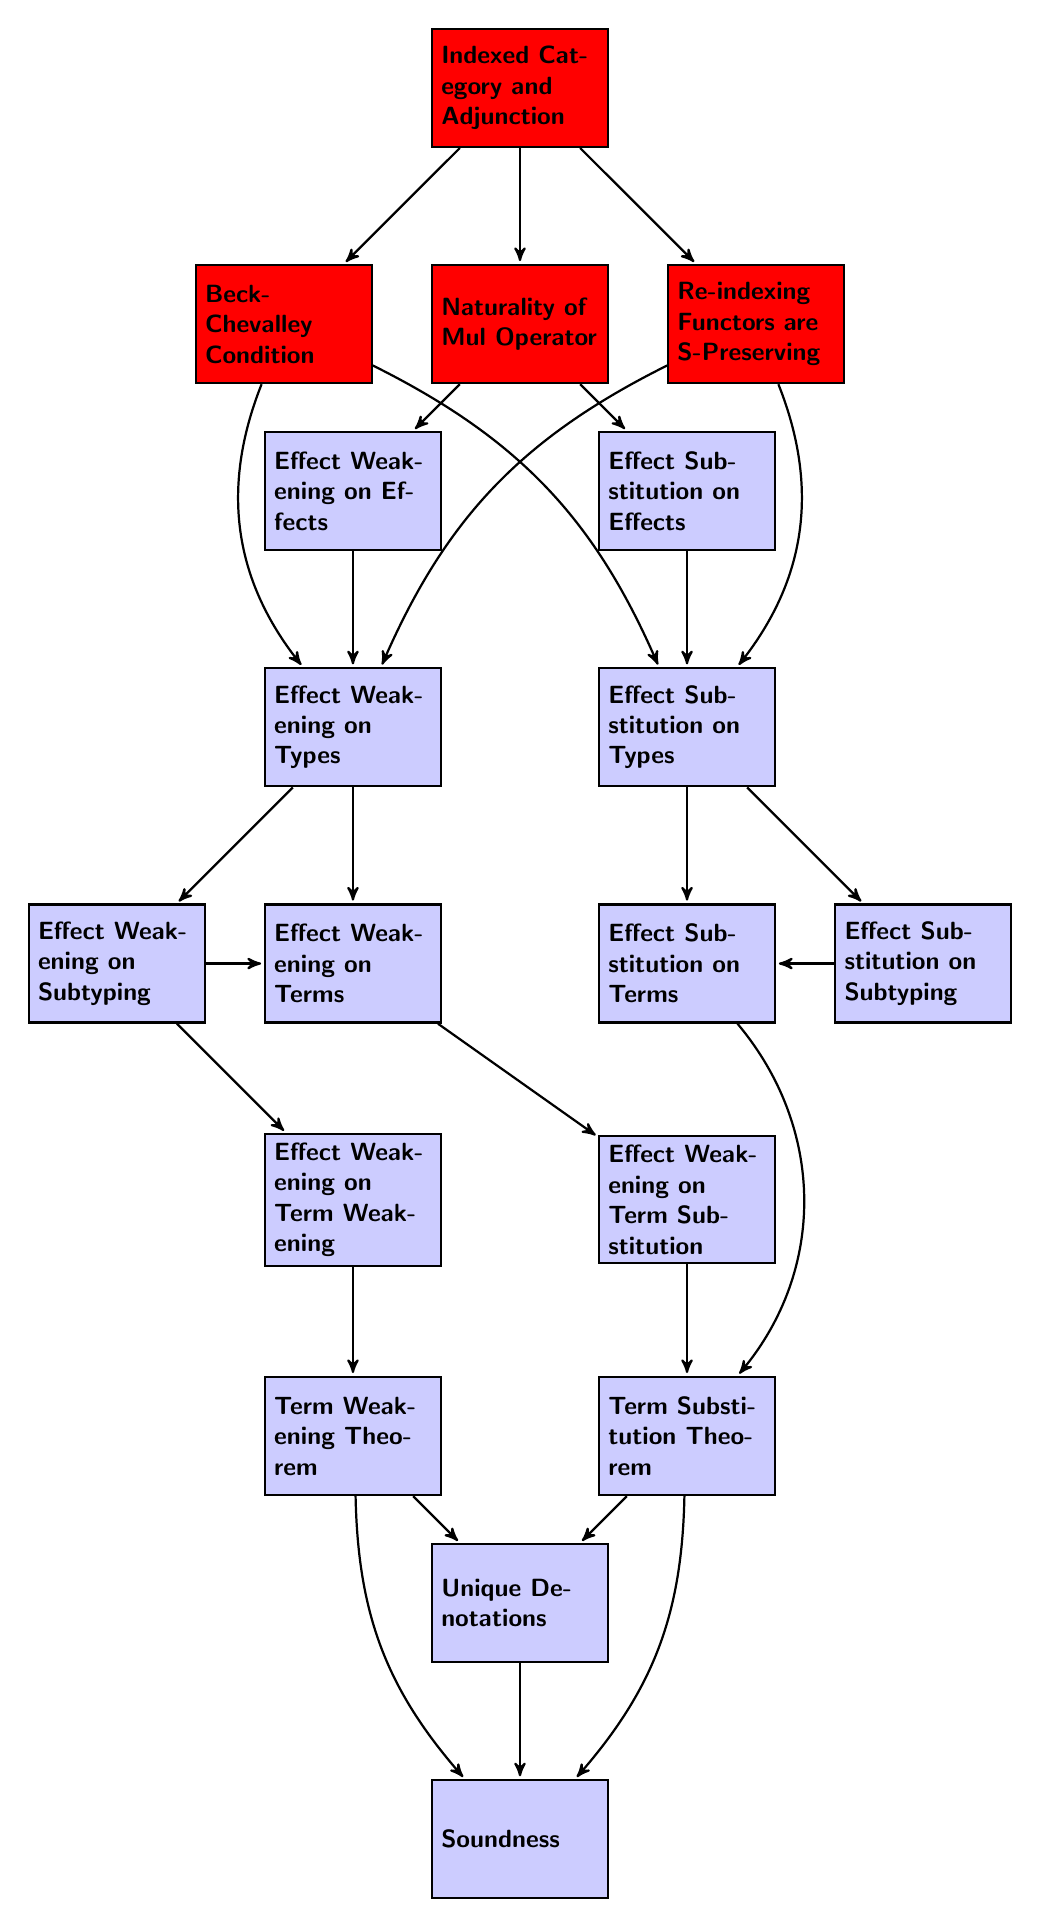
\begin{tikzpicture}[->,>=stealth',shorten >=1pt,auto,node distance=3cm,
            thick,main node/.style={rectangle,fill=blue!20,draw,
            font=\sffamily\small\bfseries,minimum size=15mm}]
        
            \node[main node,text width=20mm, fill=red] (IndexCategory) {Indexed Category and Adjunction};
            \node[main node,text width=20mm, fill=red] (MulNaturality) [below of=IndexCategory] {Naturality of Mul Operator};
        
            \node[main node,text width=20mm, fill=red] (BeckChevalley) [left of=MulNaturality]{Beck-Chevalley Condition};
            \node[main node,text width=20mm, fill=red](SClosure) [right of=MulNaturality]{Re-indexing Functors are S-Preserving};
        
            \node[main node, text width=20mm](EffectWeakeningEffects) [below left of=MulNaturality]{Effect Weakening on Effects};
        
            \node[main node, text width=20mm](EffectSubEffects) [below right of=MulNaturality]{Effect Substitution on Effects};
        
            \node[main node, text width=20mm](EffectWeakeningTypes)[below of=EffectWeakeningEffects]{Effect Weakening on Types};
        
            \node[main node, text width=20mm](EffectSubTypes)[below of=EffectSubEffects]{Effect Substitution on Types};
        
            \node[main node, text width=20mm](EffectWeakeningTerms)[below of=EffectWeakeningTypes]{Effect Weakening on Terms};
        
            \node[main node, text width=20mm](EffectSubTerms)[below of=EffectSubTypes]{Effect Substitution on Terms};
        
            \node[main node, text width=20mm](EffectWeakeningSubTyping)[left of=EffectWeakeningTerms]{Effect Weakening on Subtyping};
        
            \node[main node, text width=20mm](EffectSubSubTyping)[right of=EffectSubTerms]{Effect Substitution on Subtyping};
        
            \node[main node, text width=20mm](EffectWeakeningWeakening)[below of=EffectWeakeningTerms]{Effect Weakening on Term Weakening};
        
            \node[main node, text width=20mm](EffectWeakeningSubstitution)[below of=EffectSubTerms]{Effect Weakening on Term Substitution};
        
            \node[main node, text width=20mm](TermWeakening)[below of=EffectWeakeningWeakening]{Term Weakening Theorem};
        
            \node[main node, text width=20mm](TermSubstitution)[below of=EffectWeakeningSubstitution]{Term Substitution Theorem};
        
            \node[main node, text width=20mm](UniqueDenotations)[below left of=TermSubstitution]{Unique Denotations};
        
            \node[main node, text width=20mm](Soundness)[below of=UniqueDenotations]{Soundness};
        
            \draw [->] (IndexCategory) edge (BeckChevalley) (IndexCategory) edge (MulNaturality) (IndexCategory) edge (SClosure);
            \draw [->] (MulNaturality) edge (EffectWeakeningEffects) (MulNaturality) edge (EffectSubEffects);
        
            
            \draw [->] (EffectWeakeningEffects) edge (EffectWeakeningTypes) (EffectSubEffects) edge (EffectSubTypes);
        
            \draw [->] (EffectWeakeningTypes) edge (EffectWeakeningSubTyping) (EffectSubTypes) edge (EffectSubSubTyping);
        
            
            \draw [->] (EffectWeakeningSubTyping) edge (EffectWeakeningTerms) (EffectSubSubTyping) edge (EffectSubTerms);
        
        
            \draw [->] (EffectWeakeningTypes) edge (EffectWeakeningTerms) (EffectSubTypes) edge (EffectSubTerms);
        
            \draw [->] (EffectWeakeningTerms) edge (EffectWeakeningSubstitution) (EffectWeakeningSubTyping) edge (EffectWeakeningWeakening);
        
            \draw [->] (EffectWeakeningWeakening) edge (TermWeakening) (EffectWeakeningSubstitution) edge (TermSubstitution);
        
            \draw [->] (EffectSubTerms) edge [bend left=40] (TermSubstitution);
            \draw [->] 
                (BeckChevalley) edge [bend right=30] (EffectWeakeningTypes)
                (SClosure) edge [bend right=20] (EffectWeakeningTypes)
                (BeckChevalley) edge [bend left=20]  (EffectSubTypes)
                (SClosure) edge [bend left=30] (EffectSubTypes);
            
        
            \draw [->] (TermWeakening) edge (UniqueDenotations) (TermSubstitution) edge (UniqueDenotations) (TermWeakening) edge [bend right=20] (Soundness)
            (TermSubstitution) edge [bend left=20] (Soundness)
            (UniqueDenotations) edge (Soundness);
          \end{tikzpicture}
    }
    \end{center}
\caption{A road map of the proof dependencies. Assumptions in red, theorems in blue}
\label{RoadMap}
\end{figure}


\section{Denotations}\label{PECDenotations}
We are now equipped to define the denotations of structures in the language. Firstly, we shall define the denotation of effect environments. In the base category, with the kind of effects indicated by $U$, the denotation of an effect environment $\P$ is given by a finite product.

\[
\deno{\nil} = \1 \quad\quad \deno{\P, \a} = \deno{\P}\times U    
\]

Hence, the denotation of an  effect-variable environment $\P$ is given by a finite product on $U$ of width $n$ where $n$ is the length of $\P$. In order to de-clutter the notation used going forwards, inheriting from R. L. Crole (\cite{crole_1994}), I shall write $I$ as shorthand for $\deno{\P}$.  


As stated earlier, the denotation of a well-formed effect is a morphism $\deno{\typerelation{\P}{\e}{\effect}}: I \rightarrow U$ in $\C$.

\[
    \deno{\typerelation{\P}{e}{\effect}} = \deno{\e} \after \term{I}: I\rightarrow U
    \quad\quad
    \deno{\typerelation{\P,\a}{\a}{\effect}} = \pp: I\times U \rightarrow U
\]\[
    \deno{\typerelation{\P, \b}{\a}{\effect}} = \deno{\typerelation{\P}{\a}{\effect}}\after\p: I\times U\rightarrow U
\]\[
    \deno{\typerelation{\P}{\e_1\dot \e_2}{\effect}} = \Mul_I(\deno{\typerelation{\P}{\e_2}{\effect}},\deno{\typerelation{\P}{\e_1}{\effect}}): I \rightarrow U
\]

Using these denotations, we are now equipped to define the denotations of types. As stated above, types that are well formed in $\P$ are denoted by objects in the fibre category $\C(I)$ given by the denotation of $\P$.
 
Since the fibre category $\C(I)$ is an S-category, it has objects for all ground types, a terminal object, graded monad $\T{}{}$, exponentials, products, and co-product over $\1+\1$.

\[
    \deno{\typerelation{\P}{\U}{\type}} = \1
    \quad\quad
    \deno{\typerelation{\P}{\B}{\type}} = \1+\1
    \quad\quad
    \deno{\typerelation{\P}{\g}{\type}} = \deno{\g}
\] 

\[
    \deno{\typerelation{\P}{\ab}{\type}} = (\deno{\typerelation{\P}{B}{\type}})^{(\deno{\typerelation{\P}{A}{\type}})}
\]

\[
    \deno{\typerelation{\P}{\mea}{\type}} =\T{\deno{\typerelation{\P}{\e}{\effect}}}{\deno{\typerelation{\P}{A}{\type}}}
    \quad\quad
    \deno{\typerelation{\P}{\all{\a}{A}}{\type}} =\allI(\deno{\typerelation{\P,\a}{A}{\type}})
\]


By using the terminal objects and products present in each fibre, we can now derive denotations of type environments. $\deno{\oke{\P}{\G}}$ should be an object in the fibre induced by $\P$, $\C(I)$.

\[
    \deno{\wellformedok{\P}{\nil}} = \1
    \quad\quad
    \deno{\wellformedok{\P}{\gax}} = (\deno{\wellformedok{\P}{\G}} \times \deno{\typerelation{\P}{A}{\type}})
\]

Another construction that is important is the denotation of subtyping. For each instance of the subtyping relation in $\P$, $A\subtypep B$, there exists a denotation in the fibre induced by $\P$. $\deno{A\subtypep B} \in\C(I)(A, B)$. Since the fibres are S-categories, the ground instances of the subtyping relation exist in each fibre anyway. In addition, for each instance of the subeffect relation $\e_1\subeffectp \e_2$ each fibre contains the natural transformation $\dsep{\e_1}{\e_2}: \T{\e_1}{}\rightarrow \T{\e_2}{}$ 

\[
    \deno{\g_1\subtypep \g_2} = \deno{\g_1\subtypeg \g_2}
    \quad
    \deno{\ab \subtypep \fntype{A'}{B'}} = \deno{B\subtypep B'}^{A'}\after B^{\deno{A'\subtypep A}}
\]

\[
    \deno{\M{\e_1}{A}\subtypep\M{\e_2}{B}} = \deno{\e_1\subeffectp\e_2}\after\T{\e_1}{\deno{A\subtypep B}}
    \quad    
    \deno{\all{\a}{A}\subtypep\all{\a}{B}} = \allI{\deno{A\subtypepa B}}
\]

This finally gives us the ability to express the denotations of well-typed terms in an effect environment, $\P$ as morphisms in the fibre induced by $\P$, $\C(I)$.  Writing $\G_I$ and $A_I$ for $\deno{\wellformedok{\P}{\G}}$ and $\deno{\typerelation{\P}{A}{\type}}$, we can derive $\deno{\gpetyperelation{v}{A}}$ as a morphism in $\C(I)(\G_I, A_I)$. Since each fibre is an S-category, for each ground constant, $\const{A}$, there exists $\deno{\const{A}}: \1 \rightarrow A_I$ in $\C(I)$. These denotations can be seen in figure \ref{TermDenotations}

\begin{figure}
    \footnotesize
    \begin{framed}
        \[
            \ntreeruleI{Unit}{\wellformedok{\P}{\G}}{\deno{\etyperelation{\P}{\G}{\u}{\U}} = \term{\G} : \G_I \rightarrow \1}
            \quad
            \ntreeruleI{Const}{\wellformedok{\P}{\G}}{\deno{\etyperelation{\P}{\G}{\const{A}}{A}} = \deno{\const{A}} \after \term{\G} : \G \rightarrow \deno{A}}
        \]
        \\
        \\        
        \[
            \ntreeruleI{True}{\wellformedok{\P}{\G}}{\deno{\etyperelation{\P}{\G}{\t}{\B}} = \inl \after \term{\G} : \G \rightarrow \deno{\B} = \1+\1}
        \]
        \\
        \\
        \[
            \ntreeruleI{False}{\wellformedok{\P}{\G}}{\deno{\etyperelation{\P}{\G}{\f}{\B}} = \inr \after \term{\G} : \G \rightarrow \deno{\B} = \1+\1}
        \]
        \\
        \\        
        \[
            \ntreeruleI{Var}{\wellformedok{\P}{\G}}{\deno{\etyperelation{\P}{\gax}{x}{A}} = \pp: \G \times A \rightarrow A}
            \quad    
            \ntreeruleI{Weaken}{f = \deno{\gpetyperelation{x}{A}}: \G \rightarrow A}{\deno{\etyperelation{\P}{\gby}{x}{A}} = f \after \p: \G \times B \rightarrow A}
        \]
        \\
        \\        
        \[
            \ntreeruleI{Fn}{f = \deno{\etyperelation{\P}{\gax}{v}{B}} : \G \times A \rightarrow B}{\deno{\etyperelation{\P}{\G}{\lam{x}{A}{v}}{\ab}} = \cur{f} : \G \rightarrow (B)^A}
        \]
        \\
        \\        
        \[
            \ntreeruleII{Subtype}{f = \deno{\etyperelation{\P}{\G}{v}{A}} : \G \rightarrow A}{g = \deno{A \subtypep B}}{\deno{\etyperelation{\P}{\G}{v}{B}} = g \after f : \G \rightarrow B}
            \quad 
            \ntreeruleI{Return}{f = \deno{\etyperelation{\P}{\G}{v}{A}}}{\deno{\etyperelation{\P}{\G}{\return{v}}{\moa}} = \point{A} \after f}   
        \]
        \\
        \\        
        \[
            \ntreeruleIII{If}{f = \deno{\etyperelation{\P}{\G}{v}{\B}}: \G\rightarrow\1+\1}{g = \deno{\etyperelation{\P}{\G}{v_1}{\mea}}}{ h = \deno{\etyperelation{\P}{\G}{v_2}{\mea}}}{\deno{{\etyperelation{\P}{\G}{\ifthenelse{\e}{A}{v}{v_1}{v_2}}{\mea}}} = \app\after((\fld{\cur{g\after\pp}}{\cur{h\after\pp}}\after f)\times \idg)\after \diag{\G} : \G \rightarrow \tea}    
        \]
        \\
        \\
        \[
            \ntreeruleII{Bind}{f = \deno{\etyperelation{\P}{\G}{v_1}{\M{\e_1}{A}} : \G \rightarrow \T{\e_1}{A}}}{{ g = \deno{\etyperelation{\P}{\gax}{v_2}{\M{\e_2}{B}}}}: \G \times A \rightarrow \T{\e_2}{B}}{\deno{\etyperelation{\P}{\G}{\doin{x}{v_1}{v_2}}{\M{\e_1 \dot \e_2}{B}}} = \bind{\e_1}{\e_2}{B} \after \T{\e_1}{g} \after \tstrength{\G}{A}{\e_1} \after \pr{\idg}{f}: \G \rightarrow \T{\e_1 \dot \e_2}{B}}  
        \]
        \\
        \\        
        \[
            \ntreeruleII{Apply}{f = \deno{\gpetyperelation{v_1}{\ab}}: \G \rightarrow (B)^{A}}{g=\deno{\gpetyperelation{v_2}{A}}: \G \rightarrow A}{\deno{\gpetyperelation{\apply{v_1}{v_2}}{B}}= \app\after\pr{f}{g}: \G \rightarrow B }
        \]
        \\
        \\        
        \[
            \ntreeruleI{Effect-Gen}{f = \deno{\etyperelation{\P,\a}{\G}{v}{A}}: \ciuw(\G, A)}{\deno{\gpetyperelation{\elam{\a}{A}}{\all{\e}{A}}} = \bar{f}: \C(I)(\G, \allI(A))}    
        \] 
        \\
        \\
        \begin{equation}\label{EffectApplication}
            \ntreeruleII{Effect-Spec}{g=\deno{\gpetyperelation{v}{\all{\a}{A}}}: \C(I)(\G, \allI(A))}{ h = \deno{\typerelation{\P}{\e}{\effect}}: \ciu}{\deno{\gpetyperelation{\eapp{v}{\e}}{A\ssub{\a}{\e}}} = \pr{\Id{I}}{h}\star(\counit{\deno{\typerelation{\P,\b}{A\ssub{\a}{\b}}{\type}}})\after g: \C(I)(\G, A\ssub{\a}{\e})}
        \end{equation}                
    \end{framed}
    \caption{The denotations of terms in PEC}
    \label{TermDenotations}
\end{figure}

The least intuitive of these denotations is that of effect application (specialisation) in equation \ref{EffectApplication}. As explained later in section \ref{SubsAndWeakening} the re-indexing functor represents application of the substitution (\todo{I don't think this is circular logic, but would like another pair of eyes if possible}) $\ssub{\b}{\e}$. By doing type analysis on the co-unit morphism $ \counit{\deno{\typerelation{\P,\b}{A\ssub{\a}{\b}}{\type}}}$, as in figure \ref{CoUnitType}  we can see that before the application of the substitution, the co-unit natural transformation takes a quantified type to a substituted type under an extended effect environment. By applying the substitution re-indexing functor in figure \ref{ReIndexedCoUnitType}, we substitute $\e$ for the extra effect variable, $\b$. In the case of the quantified type, as $\b$ is not used, the substitution has no effect, but in the case of the substituted type, the substitutions compose to yield the substitution $\ssub{\a}{\e}$. This composes with the expression denotation $g$ to give the applied denotation in figure \ref{EffectSpecComp}.


\begin{figure}
    \begin{framed}
        \begin{align*}
            \counit{\deno{\typerelation{\P,\b}{A\ssub{\a}{\b}}{\type}}} & = \widehat{\Id{\allI(\deno{\typerelation{\P,\b}       {A\ssub{\a}{\b}}{\type}})}} \\ 
            & : \quad \pstar \allI(\deno{\typerelation{\P,\b}{A\ssub{\a}{\b}}{\type}}) \rightarrow \deno{\typerelation{\P,\b}       {A\ssub{\a}{\b}}{\type}} \\
            & : \quad\pstar \deno{\typerelation{\P}{\all{\b}{A\ssub{\a}{\b}}}{\type}} \rightarrow \deno{\typerelation{\P,\b}        {A\ssub{\a}{\b}}{\type}} \\
            & : \quad \pstar \deno{\typerelation{\P}{\all{\a}{A}}{\type}} \rightarrow \deno{\typerelation{\P,\b}{A\ssub     {\a}{\b}}{\type}}\\
            & : \quad \deno{\typerelation{\P, \b}{\all{\a}{A}}{\type}} \rightarrow \deno{\typerelation{\P,\b}{A\ssub{\a}{\b}}{\type}}
        \end{align*}
    \end{framed}
    \caption{Analysis of the type of the co-unit natural transformation}
    \label{CoUnitType}
\end{figure}

\begin{figure}
    \begin{framed}
        \begin{align*}
            \pr{\Id{I}}{h}\star(\counit{\deno{\typerelation{\P,\b}{A\ssub{\a}{\b}}{\type}}}) & : \quad \deno{\typerelation{\P}{\all{\a}{A}}{\type}} \rightarrow \deno{\typerelation{\P}{A\ssub{\a}{\b}\ssub{\b}{\e}}{\type}}\\
            & : \quad \deno{\typerelation{\P}{\all{\a}{A}}{\type}} \rightarrow \deno{\typerelation{\P}{A\ssub{\a}{\e}}{\type}}
        \end{align*}
    \end{framed}
    \caption{Analysis of the type of the re-indexed co-unit}
    \label{ReIndexedCoUnitType}
\end{figure}


 
\begin{figure}
    \begin{framed}
        \centering
        \begin{tikzcd}
            &  \deno{\typerelation{\P, \b}{\all{\a}{A}}{\type}}  \arrow{rrrr}{\counit{\deno{\typerelation{\P,\b}{A\ssub{\a}{\b}}{\type}}}}&&&&  \deno{\typerelation{\P,\b}{A\ssub{\a}{\b}}{\type}} &
            \\
            \G \arrow{rr}{g}&&
            \allI (A) \arrow{rrrr}{ \pr{\Id{I}}{h}\star(\counit{\deno{\typerelation{\P,\b}{A\ssub{\a}{\b}}{\type}}})}
            &&&&
            A\ssub{\a}{\e}
        \end{tikzcd}
    \end{framed}
    \caption{Composition of the effect specialisation denotation}
    \label{EffectSpecComp}
\end{figure}



\section{Substitution and Weakening Theorems}\label{SubsAndWeakening}

In this section, I introduce and prove a series of utility theorems, which will help us prove cases in future theorems. These weakening and substitution theorems are concerned with a change in environment of typing derivations and their associated denotations. If $\gpetyperelation{v}{A}$, then it should be the case that $\etyperelation{\P}{\gax}{v}{A}$ if $x$ is fresh in $\G$. We also want to know what happens to the denotation when we change the type environment in this way. In this section, I introduce the tools for manipulating the type and effect environments in this way.

Substitutions and weakenings are two distinct ways of manipulating an effect or term environments. Weakening acts as a kind of subtyping of the environment. If we insert fresh variables into an environment, then any expression that was typeable under the previous environment should also be typeable under the the new environment. This change of environment should also have a predictable effect on the denotations of any expressions to which it is applied.

Substitution considers what happens when we simultaneously replace all variables in one expression, that is typeable under an environment, with expressions that are well formed under another environment. The resulting substituted expression should be typeable under the new environment, and the denotation of the new expression should be composed from the denotation of the old relation and the denotations of the expressions that replace the variables. 

As we go on, I shall define and state the denotations of specific substitutions and weakenings, upon both the effect environment and the term environments.

In this dissertation, substitutions and weakenings come in two flavours: weakening and substitution of the effect-variable environment and weakening and substitution of the term environments. For each of these there is a family of theorems defining the effects of the applying a substitution and weakening to the various language structures and their denotations, such as well-formedness and typing relations.


The first family of theorems is that of weakening and substitution of the effect environment. Weakenings are a relation between effect environments $\wrel{\w}{\P'}{\P}$, that are defined as so:

\[
    \ntreeruleI{Id}{\ok{\P}}{\wrel{\i}{\P}{\P}}
    \quad
    \condtreeruleI{Project}{\wrel{\w}{\P'}{\P}}{\wrel{\w\pi}{(\P', \a)}{\P}}{\a\notin\P'}
    \quad
    \condtreeruleI{Extend}{\wrel{\w}{\P'}{\P}}{\wrel{\w\x}{(\P', \a)}{(\P, \a)}}{\a\notin\P'}
\]

We can define the denotation of an effect-environment weakening as a morphism in the base category: $\deno{\wrelw{\P'}{\P}}: I' \rightarrow I$. The denotations are defined as follows:

\[
    \deno{\wrel{\i}{\P}{\P}} = \Id{I}: I \rightarrow I
    \quad
    \deno{\wrel{\w\pi}{\P',\a}{\P}} = \deno{\wrelw{\P'}{\P}}\after \p: I'\times U\rightarrow I
\]

\[
    \deno{\wrel{\w\x}{\P',\a}{\P,\a}} = (\deno{\wrelw{\P'}{\P}}\times \Id{U}): I'\times U\rightarrow I\times U    
\]

Substitutions are also an inductively defined relation between effect environments, with inductively defined denotations. Substitutions may be represented as a snoc-list of variable-effect pairs.

\[
    \si \gens \nil \mid \si, \a \setto \e    
\]

The substitution relation matches substitutions to the environments it operates between. The relation instance $\typerelation{\P'}{\si}{\P}$ means that $\si$ is a substitution from $\P'$ to $\P$. It is defined inductively using the following rules.

\[
    \ntreeruleI{Nil}{\ok{\P'}}{\typerelation{\P'}{\nil}{\nil}}
    \quad\quad
    \condtreeruleII{Extend}{\typerelation{\P'}{\si}{\P}}{\wellformed{\P'}{\e}}{\typerelation{\P'}{\si, \a \setto\e}{(\P, \a)}}{\a\notin\P}
\]

The denotation of an effect-environment substitutions, $\deno{\typerelation{\P'}{\si}{\P}}$, is a morphism $I' \rightarrow I$ in the base category. These denotations are defined inductively as so:

\[
    \deno{\typerelation{\P'}{\nil}{\nil}} = \term{I}: \C(I', \1)
    \quad\quad
    \deno{\typerelation{\P'}{(\si, \a\setto\e)}{\P,\a}} = \pr{\deno{\typerelation{\P'}{\si}{\P}}}{\deno{\typerelation{\P}{\e}{\effect}}}: \C(I', I\times U)
\]

We can also define the action of substitutions on effects.

\begin{align*}
    \si(e) & = e \\
    \si(\e_1\dot\e_2) & = (\si(\e_1))\dot(\si(\e_2))\\
    \nil(\a) & = \a\\
    (\si, \b\setto \e)(\a) & = \si(\a) \\
    (\si, \a\setto \e)(\a) & =\e
\end{align*}.

The general construction for effect-variable substitution allows us to define, in particular, the identity substitution, $\typerelation{\P}{\Id{\P}}{\P}$ and the single substitution, $\typerelation{\P}{\ssub{\a}{\e}}{\P,\a}$.


\begin{align}\label{SpecialSubs}
    \Id{\nil} & = \nil\\
    \Id{\P,\a} & = (\Id{\P}, \a\setto\a)\\
    \ssub{\a}{\e} & = (\Id{\P}, \a\setto \e)
\end{align}

By inspection, we can find the denotations of these special-case substitutions to be:

\begin{align}\label{SpecialSubsDenotations}
    \deno{\typerelation{\P}{\Id{\P}}{\P}} & = \Id{I}\\
    \deno{\typerelation{\P}{\ssub{\a}{\e}}{(\P,\a)}} & = \pr{\Id{I}}{\deno{\typerelation{\P}{\e}{\effect}}}
\end{align}


These substitutions will form a useful shorthand later. We also need to define the property $\a \# \si$. This indicates that $\a$ does not occur in the domain or any of the substitution expression of $\si$. Finally, it will be useful to examine how the substitutions generated by extending the effect environment, such as in the case of polymorphic types, relate to the original substitution.




\begin{theorem}[Effect Substitution on Effects]
    The substitution theorem on effects is the proposition that if $\wellformed{\P}{\e}$ and $\typerelation{\P'}{\si}{\P}$ then $\wellformed{\P'}{\si(\e)}$ and, writing $\si$ for $\deno{\typerelation{\P'}{\si}{\P}}$,  $\deno{\wellformed{\P'}{\si(\e)}} = \deno{\wellformed{\P}{\e}}\after\si$. 
\end{theorem}


\begin{proof}
    The proof of this depends on the naturality of $\Mul_I$ and inversion to narrow down case splitting on the structure of the effect environments.

    \case{Ground}
    This case holds due to the terminal morphism being unique. Hence, pre-composing it with another morphism yields the terminal morphism.

    \begin{align*}
        \deno{\typerelation{\P}{e}{\effect}}\after\si & = \deno{e}\after\term{I}\after\si \\
        & = \deno{e}\after\term{I'} \\
        & = \deno{\typerelation{\P'}{e}{\type}}\\
    \end{align*}

\case{Var}

Since the structure of the substitution $\si$ depends on the structure of $\P$, we can perform inversion to infer the denotation of $\si$.

\begin{align*}
    \deno{\typerelation{\P,\a}{\a}{\effect}}\after\si &= \pp\after\pr{\si'}{\deno{\typerelation{\P'}{\e}{\effect}}}\qt{By inversion $\si = (\si', \a\setto\e)$}\\
    & =\deno{\typerelation{\P'}{\e}{\effect}} \\
    &= \deno{\typerelation{\P'}{\si'(\a)}{\effect}}\\
\end{align*}


\case{Compose}

We make use of the naturality of $\Mul_I$ and induction upon the subterms.
\begin{align*}
    \deno{\typerelation{\P}{\e_1\dot\e_2}{\effect}} \after\si &=
    \Mul_I(\deno{\typerelation{\P}{\e_1}{\effect}}, \deno{\typerelation{\P}{\e_2}{\effect}})\after \si \\
    & = \Mul_I(\deno{\typerelation{\P}{\e_1}{\effect}}\after \si, \deno{\typerelation{\P}{\e_2}{\effect}}\after \si)\qt{By Naturality}\\
    & = \Mul_{I'}(\deno{\typerelation{\P'}{\si(\e_1)}{\effect}}, \deno{\typerelation{\P}{\si(\e_2)}{\effect}})\\
    & = \deno{\typerelation{\P'}{\si(\e_1)\dot\si(\e_2)}{\effect}}\\
    & = \deno{\typerelation{\P'}{\si(\e_1\dot\e_2)}{\effect}}\\
\end{align*}

$$\square$$
\end{proof}


\begin{theorem}[Effect Weakening on Effects]\label{EffWeakeningEff}
    The weakening theorem proceeds similarly. If $\wellformed{\P}{\e}$ and $\wrelw{\P'}{\P}$ then $\wellformed{\P'}{\w}$ and, writing $\w$ for $\deno{\wrelw{\P'}{\P}}$,  $\deno{\wellformed{\P'}{\e}} = \deno{\wellformed{\P}{\e}}\after\w$.

\end{theorem}

\begin{proof}
    This proof also depends on the naturality of $\Mul_I$ and case splitting on the structure of $\w$. It is harder to use inversion on the structure of $\w$, since the structure of $\w$ does not depend as strongly on the structure of $\P$. I present here the cases for variables.

    \case{Var}
    We do a case split on $\w$.
    \subcase{$\w = \i$}
    Then $\P' = \P$ and $\w = \Id{I}$. So the theorem holds trivially.
    \subcase{$\w = \w'\x$}
    Then by the definition of its denotation:    
    \begin{align*}
        \deno{\typerelation{\P,\a}{\a}{\effect}}\after\w &= \pp\after(\w'\times \Id{U}) \\
        & = \pp\\
        & = \deno{\typerelation{\P',\a}{\a}{\effect}}
    \end{align*}
    
    \subcase{$\w = \w'\pi$}
    Then \begin{equation}
        \deno{\typerelation{\P,\a}{\a}{\effect}} = \pp\after\w'\after\p
    \end{equation}
    
    Where $\P' = \P,\b$ and $\wrel{\w'}{\P''}{\P}$.
    
    So\begin{align*}
        \pp\after\w' & = \deno{\typerelation{\P''}{\a}{\effect}}
        \\
        \pp\after\w'\after\p & =\deno{\typerelation{\P'',\b}{\a}{\effect}}\\
        &= \deno{\typerelation{\P'}{\a}{\effect}}
    \end{align*}
    
    \case{Weaken}
    \begin{equation}
        \deno{\typerelation{\P,\b}{\a}{\effect}}\after\w = \deno{\typerelation{\P}{\a}{\effect}}\after\p\after\w
    \end{equation}
    
    Similarly, we perform a case split on structure of $\w$:
    
    \subcase{$\w=\i$}
    Then $\P' = \P,\b$ so $\w=\Id{I}$
    So $\deno{\typerelation{\P,\b}{\a}{\effect}}\after\w = \deno{\typerelation{\P'}{\a}{\effect}}$
    
    \subcase{$\w=\w'\p$}
    Then $\P' = (\P'',\g)$ and $\w=\w'\after\p$
    Where $\wrel{\w'}{\P''}{\P,\b}$.
    So
    \begin{align*}
        \deno{\typerelation{\P,\b}{\a}{\effect}}\after\w & = \deno{\typerelation{\P,\b}{\a}{\effect}}\after\w'\after\p\\
        & = {\typerelation{\P''}{\a}{\effect}}\after\p\\
        & = {\typerelation{\P'',\g}{\a}{\effect}}\\
        & = {\typerelation{\P'}{\a}{\effect}}\\
    \end{align*}
    
    \subcase{$\w=\w'\x$}
    Then $\P'=\P'',\b$ and $\wrel{\w'}{\P''}{\P}$
    
    So \begin{align*}
        \deno{\typerelation{\P,\b}{\a}{\effect}}\after\w &= \deno{\typerelation{\P}{\a}{\effect}}\after\p\after(\w'\times\Id{U})\\
        &=\deno{\typerelation{\P}{\a}{\effect}}\after\w'\after\p\\
        & = \deno{\typerelation{\P''}{\a}{\effect}}\after\p\\
        & = \deno{\typerelation{\P'}{\a}{\effect}}\\
    \end{align*}

    $$\square$$
\end{proof}

\begin{lemma}[Extension Lemma on Effect Substitutions]
    If $\typerelation{\P'}{\si}{\P}$, and $\a\#\si$, then $\typerelation{(\P', \a)}{(\si, \a\setto\a)}{(\P,\a)}$ with denotation $\deno{\typerelation{(\P', \a)}{(\si, \a\setto\a)}{(\P,\a)}} = (\deno{\typerelation{\P'}{\si}{\P}}\times\Id{U})$
\end{lemma}
\begin{proof}
   This holds by the weakening-theorem on effects, theorem \ref{EffWeakeningEff}

   $$\square$$
\end{proof}



We can then move on to state and prove the weakening and substitution theorems on types, subtyping, and type environments. The general structure of these theorems, as well as the term-based theorems later, is that when we want to quantify the action of a morphism $\theta: I' \rightarrow I$ between objects in the base category on structure in the fibres $\C(I)$, we should simply apply the associated re-indexing functor $\theta\star: \C(I) \rightarrow \C(I')$ to the structure. The proof of the soundness of this operation is driven by the fact that the re-indexing functor is S-preserving.

Specifically, effect substitutions have the following actions on types, and type-environments:

\begin{align*}
    \g\sub{\si} &= \g \\
    (\fntype{A}{B})\sub{\si} &= \fntype{(A\sub{\si})}{(B\sub{\si})} \\
    (\M{\e}{A})\ssi &= \M{\si(\e)}{(A\ssi)}\\
    (\all{\a}{A})\ssi &= \all{\a}{(A\ssi)}\qt{If $\a\#\si$}
\end{align*}

\begin{align*}
    \nil\ssi & = \nil \\
    (\gax)\ssi &= (\G\ssi, x:(A\ssi))\\
\end{align*}


\begin{theorem}[Effect Substitution on Types]
    The specific effect substitution theorem on types is if $\wellformed{\P}{A}$ and $\typerelation{\P'}{\si}{\P}$, then $\wellformed{\P'}{A\ssi}$ and $\deno{\wellformed{\P'}{A\ssi}} = \si\star\deno{\wellformed{\P}{A}}$.
\end{theorem}

\begin{proof}
   By the fact that $\si\star$ is S-preserving and the Beck-Chevalley Condition.

    \case{Effect}
    This case makes use of the fact that $\si\star$ is S-preserving. Specifically the property upon the graded monad functor $\T{}{}$: $\si\star(\T{f}{A}) = \T{f\after\si}{(\si\star A)}$.


    \begin{align*}
        \si\star\deno{\typerelation{\P}{\mea}{\type}} & =  \si\star(\T{\deno{\typerelation{\P}{\e}{\effect}}}{\deno{\typerelation{\P}{A}{\type}}})\\
        &= \T{\deno{\typerelation{\P}{\e}{\effect}}\after\si}{\si\star(\deno{\typerelation{\P}{A}{\type}})}\\
        & = \deno{\typerelation{\P'}{(\mea)\ssi}{\type}}
    \end{align*}
    \case{Quantification}
    This case makes use of the Beck-Chevalley condition and the fact that $\deno{\typerelation{(\P', \a)}{(\si, \a\setto\a)}{(\P, \a)}} = \si\times\Id{U}$, which we can induct upon.
        \begin{align*}
            \si\star\deno{\typerelation{\P}{\all{\a}A}{\type}} & = \si\star(\allI(\deno{\typerelation{\P,\a}{A}{\type}}))\\
            & = \allI((\si\times\Id{U})\star\deno{\typerelation{\P,\a}{A}{\type}})\qt{By Beck-Chevalley}\\
            & = \allI(\deno{\typerelation{\P',\a}{A\sub{\si, \a\setto\a}}{\type}})\qt{By induction}\\
            & = \deno{\typerelation{\P'}{\all{\a}{(A\sub{\si, \a\setto\a})}}{\type}}\\
            & = \deno{\typerelation{\P'}{(\all{\a}{A})\ssi}{\type}}\\
        \end{align*}
        $$\square$$
\end{proof}

\begin{theorem}[Effect Substitution on Type Environments]
    Similarly, the effect-substitution theorem on type environments is that if $\wellformedok{\P}{\G}$, then $\wellformedok{\P'}{\G\ssi}$ and $\deno{\wellformedok{\P'}{\G\ssi}} = \si\star\deno{\wellformedok{\P}{\G}}$.
\end{theorem}

\begin{proof}
    By induction on the derivation on $\deno{\wellformedok{\P}{\G}}$ whilst making use of the S-preserving property of the re-indexing functor.

    \case{Nil}
    We make use of the fact that an S-preserving functor preserves the terminal object.
    \begin{align*}
        \si\star\deno{\wellformedok{\P}{\nil}} &=\si\star\1\\
        & = \1\qt{By S-preserving property}\\
        &= \deno{\wellformedok{\P'}{\nil}}\\
        &= \deno{\wellformedok{\P'}{\nil\ssi}}\\
    \end{align*}
    
    \case{Extend}
    The S-preserving property means that $\si\star(A \times B) = (\si\star A)\times (\si\star B)$.
    \begin{align*}
       \si\star\deno{\wellformedok{\P}{\gax}} &= \si\star(\deno{\wellformedok{\P}{\G}} \times \deno{\typerelation{\P}{A}{\type}}) \\
       & = (\si\star\deno{\wellformedok{\P}{\G}} \times \si\star\deno{\typerelation{\P}{A}{\type}})\\
        & = (\deno{\wellformedok{\P'}{\G\ssi}} \times \deno{\typerelation{\P'}{A\ssi}{\type}})\\
        & = \deno{\wellformedok{\P'}{\G\ssi, x: A\ssi}}\\
        & = \deno{\wellformedok{\P'}{(\gax)\ssi}}\\
    \end{align*}

    $$\square$$
\end{proof}


The effect-weakening theorem on types and type environments is also very similar.

\begin{theorem}[Effect Weakening on Types]
    If $\wrelw{\P'}{\P}$ and $\wellformed{\P}{A}$ then $\wellformed{\P'}{A}$ $\deno{\wellformed{\P'}{A}} = \w\star\deno{\wellformed{\P}{A}}$. Further more, $\wrelw{\P'}{\P}$ and $\wellformedok{\P}{\G}$ imply $\deno{\wellformedok{\P'}{\G}} = \w\star\deno{\wellformedok{\P}{\G}}$
\end{theorem}

\begin{proof}
   In a similar fashion, we make use of the Beck-Chevalley condition and the S-preserving property of $\si\star$.

    \case{Quantification}
        This case uses the Beck-Chevalley condition and the fact that $\deno{\wrel{\w\x}{(\P', \a)}{(\P,\a)}} = \w\times \Id{U}$. This property is used in conjunction with induction to change the environment from $(\P, \a)$ to $(\P', \a)$.

        \begin{align*}
            \w\star\deno{\typerelation{\P}{\all{\a}A}{\type}} & = \w\star(\allI(\deno{\typerelation{\P,\a}{A}{\type}}))\\
            & = \allI((\w\times\Id{U})\star\deno{\typerelation{\P,\a}{A}{\type}})\qt{By Beck-Chevalley}\\
            & = \allI(\deno{\typerelation{\P',\a}{A}{\type}})\qt{By induction}\\
            & = \allI(\deno{\typerelation{\P',\a}{A}{\type}})\\
            & = \deno{\typerelation{\P'}{\all{\a}{A}}{\type}}\\
        \end{align*}
    
    \case{Fn}
    This case makes use of the S-preserving property that $\w\star$ preserves exponentials. Specifically $\w\star(B^A) = (\w\star B)^{(\w\star A)}$.
    \begin{align*}
        \w\star\deno{\typerelation{\P}{\ab}{\type}} &= \w\star(\deno{\typerelation{\P}{B}{\type}}^{\deno{\typerelation{\P}{A}{\type}}})\\
        &=\w\star(\deno{\typerelation{\P}{B}{\type}})^{\w\star(\deno{\typerelation{\P}{A}{\type}})}\\
        & = \deno{\typerelation{\P'}{B}{\type}}^{\deno{\typerelation{\P'}{A}{\type}}}\\
        & = \deno{\typerelation{\P'}{\ab}{\type}}\\
    \end{align*}

    
    The proof for type environments follows the same steps as effect-substitution proof.

    $$\square$$
\end{proof}


Next we consider the action of weakening and substitution on subtyping relations. 

\begin{theorem}[Effect Substitution on Subtyping]
    If $A$ is a subtype of $B$ under environment $\P$ ($A \subtypep B$), and $\si$ is a substitution from $\P'$ to $\P$ ($\typerelation{\P'}{\si}{\P}$), then $A\ssi$ is also a subtype of $B\ssi$ under $\P'$ ($A\ssi\subtypepp B\ssi$) and $\deno{A\ssi\subtypepp B\ssi} = \si\star\deno{A\subtypep B}$.
\end{theorem}

\begin{proof}
    By rule induction over the definition of the subtype relation, making use of S-preserving property and the effect-substitution theorem on types.


\case{Ground}
This case holds by the property of the S-preserving property of $\si\star$ that $\si\star$ preserves the ground-type subtyping denotation.

\begin{align*}
    \si\star(\g_1\subtypeg\g_2) &= (\g_1\subtypeg\g_2)
\end{align*}



\case{Fn}

This case holds by several S-preserving properties of $\si\star$. $\si\star$ preserves the exponential morphisms: $\si\star(\cur{f}) = \cur{\si\star(f)}$ and $\si\star(\app) = \app$. $\si\star$ should also preserve the product morphisms: $\si\star(\p) = \p$, $\si\star(\pp) = \pp$ and $\si\star\pr{f}{g} = \pr{\si\star f}{\si\star g}$. Hence $\si\star(f \times g) = (\si\star f \times \si\star g)$.

\begin{align*}
    \si\star\deno{(\ab)\subtypep\fntype{A'}{B'}} &= \si\star(\deno{B\subtypep B'}^{A'}\after B^{\deno{A'\subtypep A}})\\
    &= \si\star(\cur{\deno{B\subtypep B'}\after\app})\after\si\star(\cur{\app\after(\Id{B}\times\deno{A'\subtypep A})})\\
    & = \cur{\si\star(\deno{B\subtypep B'})\after\app}\after\cur{\app\after(\Id{B}\times\si\star(\deno{A'\subtypep A}))}\\
    & = \cur{\deno{B\ssi\subtypepp B'\ssi}\after\app}\after\cur{\app\after(\Id{B\ssi}\times\deno{A'\ssi\subtypepp A\ssi})}\\
    &= \deno{\fntype{(A\ssi)}{(B\ssi)}\subtypepp\fntype{(A'\ssi)}{(B'\ssi)}}\\
    &= \deno{(\ab)\ssi\subtypepp(\fntype{A'}{B'})\ssi}
\end{align*}


$$\square$$
\end{proof}


Similarly we can form the symmetrical weakening theorem.

\begin{theorem}[Effect Weakening on Subtyping]
    If $A \subtypep B$ and $\wrelw{\P'}{\P}$, then $A \subtypepp B$ and $\deno{A\subtypepp B} = \w\star\deno{A\subtypep B}$.
\end{theorem}



\begin{proof}
    The cases hold the same as in the corresponding substitution theorem.

    $$\square$$
\end{proof}



We are now at a point to define and prove the effect weakening and substitution theorems on terms. Following the intuition above that changes of index object should be modelled by applying the re-indexing functor to the morphisms denoting the terms, we can construct the theorems. Firstly, we must define the operation of effect substitutions on terms.

\begin{align*}
    x\ssi & = x \\
    \const{A}\ssi & = \const{(A\ssi)} \\
    (\lam{x}{A}{v})\ssi &= \lam{x}{(A\ssi)}{(v\ssi)}\\
    (\pifthenelse{A}{v}{v_1}{v_2})\ssi &= \pifthenelse{(A\ssi)}{v\ssi}{v_1\ssi}{v_2\ssi}\\
    (\apply{v_1}{v_2})\ssi&= \apply{(v_1\ssi)}{v_2\ssi}\\
    (\doin{x}{v_1}{v_2})\ssi&= \doin{x}{(v_1\ssi)}{(v_2\ssi)}\\
    (\elam{\a}{v})\ssi & = \elam{\a}{(v\ssi)}\qt{If $\a\#\si$}\\
    (\eapp{v}{\e})\ssi & = \eapp{(v\ssi)}{\si(\e)}\\
\end{align*}

The substitution theorem is defined as so:

\begin{theorem}[Effect Substitution on Terms]
    If $\typerelation{\P'}{\si}{\P}$ and typing derivation tree $\D$ derives $\gpetyperelation{v}{A}$ then there exists a typing derivation tree  $\D'$ deriving $\etyperelation{\P'}{\G\ssi}{v\ssi}{A\ssi}$ and $\D' = \si\star(\D)$.
\end{theorem}


\begin{proof}
    This proof makes use of the previous effect-substitution theorems, and the adjunction of quantification and the re-indexing functor of projection, $\pstar$.

    \case{Effect-Gen}

This case makes use of the naturality condition \ref{NaturalityCondition} and simple reductions. 
If $\D$ derives $\gpetyperelation{\elam{\a}{v}}{\all{\a}{A}}$ then by inversion, there exists $\D_1$ deriving  $\etyperelation{\P,\a}{\G}{v}{A}$ such that $\D = \bar{\D_1}$. By the extension lemma, we can pick $\a\notin\P'\wedge\a\notin\P$ so that we have: $\typerelation{(\P',\a)}{(\si, \a\setto\a)}{(\P,\a)}$. By induction, there exists $\D_1'$ deriving $\etyperelation{(\P', \a)}{\G\sub{\si, \a\setto\a}}{v\sub{\si,\a\setto\a}}{A\sub{\si, \a\setto\a}}$, which we can simplify to $\etyperelation{\P',\a}{\G\ssi}{v\ssi}{A\ssi}$ since $\a$ does not occur in $\P$ or $\P'$. Hence $\etyperelation{\P'}{\G\ssi}{v\ssi}{(\all{\a}{A})\ssi}$ by the tree given in equation \ref{EffectSubTermsEffectLambda} ($\D'$).

\begin{equation}\label{EffectSubTermsEffectLambda}
    \D' = \ntreeruleI{Effect-Gen}{\treeruleI{\D_1'}{\etyperelation{\P',\a}{\G\ssi}{v\ssi}{A\ssi}}}{\etyperelation{\P'}{\G\ssi}{v\ssi}{(\all{\a}{A})\ssi}}
\end{equation}

It is also the case that:

\begin{equation}
    \si\times\Id{} = \deno{\typerelation{(\P',\a)}{(\si, \a\setto\e)}{(\P,\a)}}
\end{equation}

So
\begin{align*}
    \si\star\D &= \si\star(\bar{\D_1})\\
    & = \bar{(\si\times\Id{U})\star\D_1}\qt{By naturality}\\
    & = \bar{\D_1'}\qt{By induction}\\
    & = \D'
\end{align*}

\case{Effect-Spec}

This is a more complex case, as it makes use of several naturality properties and the adjunction $\pstar\dashv\allI$. By inversion, if $\D$ derives $\gpetyperelation{\eapp{v}{\e}}{A\ssub{\a}{\e}}$ then there exists $\D_1$ deriving $\gpetyperelation{v}{\all{\a}{A}}$ and $h = \deno{\typerelation{\P}{\e}{\effect}}$ such that $\D$ is derived from $\D_1$ and $h$ as in equations \ref{EffectSubTermsEffAppTree} and \ref{EffectSubTermsEffAppDeno}.


\begin{equation}\label{EffectSubTermsEffAppTree}
    \D = \ntreeruleII{Effect-Spec}{\treeruleI{\D_1}{\gpetyperelation{v}{\all{\a}{A}}}}{\treeruleI{h}{\typerelation{\P}{\e}{\effect}}}{\gpetyperelation{\eapp{v}{\e}}{A\ssub{\a}{\e}}}
\end{equation}
\begin{equation}\label{EffectSubTermsEffAppDeno}
    \D = \pr{\Id{\G}}{h}\star(\e_{\deno{\typerelation{\P,\b}{A\ssub{\a}{\b}}{\type}}})\after\D_1
\end{equation}

So by induction and effect-substitution preserving well-formedness of effects, we have $\D_1'$ deriving $\etyperelation{\P'}{\G\ssi}{v\ssi}{(\all{\a}{A})\ssi}$ and $\wellformed{\P'}{\si(\e)}$. Using the Effect-Spec type rule, we can construct $\D'$ deriving $\etyperelation{\P'}{\G\ssi}{\eapp{(v\ssi)}{(\si(\e))}}{A\ssi\ssub{\a}{\si(\e)}}$ from $\D_1'$, as in equation \ref{EffectSubTermsEffAppNewTree}. Since $\a\#\si$, we can commute the applications of substitution. As a result, $\D'$ also derives $\etyperelation{\P'}{\G\ssi}{(\eapp{v}{\e})\ssi}{A\ssub{\a}{\e}\ssi}$.


\begin{equation}
    \label{EffectSubTermsEffAppNewTree}
    \D' = \ntreeruleII{Effect-Spec}{
    \treeruleI{\D_1'}{\etyperelation{\P'}{\G\ssi}{v\ssi}{(\all{\a}{A})\ssi}}
    }{
    \wellformed{\P'}{\si(\e)}
    }{\etyperelation{\P'}{\G\ssi}{\eapp{(v\ssi)}{(\si(\e))}}{A\ssi\ssub{\a}{\si(\e)}}}
\end{equation}



So, due to the substitution theorem on effects,
\begin{equation}
    h\after\si = \deno{\typerelation{\P}{\e}{\effect}}\after\si = \deno{\typerelation{\P'}{\si(\e)}{\effect}} = h'
\end{equation}

Hence, by applying the re-indexing functor to $\D$, we have:

\begin{align*}
    \si\star{\D} & = \si\star(\pr{\Id{\G}}{h}\star(\e_{\deno{\typerelation{\P,\b}{A\ssub{\a}{\b}}{\type}}})\after\D_1)\\
    & = (\pr{\Id{\G}}{h}\after\si)\star(\e_{\deno{\typerelation{\P,\b}{A\ssub{\a}{\b}}{\type}}})\after\si\star(\D_1)\\
    & = ((\si\times\Id{U})\after\pr{\Id{\G}}{h\after\si})\star(\e_{\deno{\typerelation{\P,\b}{A\ssub{\a}{\b}}{\type}}})\after\D_1'\\
    & = (\pr{\Id{\G}}{h'})\star((\si\times\Id{U})\star\e_{\deno{\typerelation{\P,\b}{A\ssub{\a}{\b}}{\type}}})\after\D_1'
\end{align*}

Looking at the inner part of the functor application:
Let \begin{align*}
    A & = \deno{\typerelation{\P,\b}{A\ssub{\a}{\b}}{\type}}\\
\end{align*}
\begin{align*}
    (\si\times\Id{U})\star\e_{\deno{\typerelation{\P,\b}{A\ssub{\a}{\b}}{\type}}} &= (\si\times\Id{U})\star\counit{A}\\
    & = (\si\times\Id{U})\star(\widehat{\Id{\allI(A)}})\\
    & = \widehat{\bar{(\si\times\Id{U})\star(\widehat{\Id{\allI(A)}})}}\qt{By bijection}\\
    & = \widehat{\si\star(\bar{\widehat{\Id{\allI(A)}}})}\qt{By naturality}\\
    & = \widehat{\si\star(\Id{\allI(A)})}\qt{By bijection}\\
    & = \widehat{\Id{\allII(A\after(\si\times\Id{U}))}}\qt{By S-preserving property, naturality}\\
    & = \widehat{\Id{\allII(A\sub{\si,\a\setto\a})}}\qt{By Substitution theorem}\\
    & = \e_{A\ssi}
\end{align*}

Going back to the original expression:

\begin{align*}
    \si\star{\D} & = (\pr{\Id{\G}}{h'})\star(\e_{A\ssi})\after\D_1')\\
    & = \D'
\end{align*}
$$\square$$
\end{proof}


 
\begin{theorem}[Effect Weakening on Terms]
   Similarly, we can derive the weakening theorem on terms.

    If $\wrelw{\P'}{\P}$ and $\D$ derives $\gpetyperelation{v}{A}$ then there exists $\D'$ deriving $\etyperelation{\P'}{\G}{v}{A}$ and $\D' = \w\star\D$.
\end{theorem}

\begin{proof}
    This theorem is proved in a similar fashion to the substitution theorem, and many of its cases are the same.


    \case{Subtype}
    If $\D$ derives $\gpetyperelation{v}{B}$ then, by inversion, there exists $\D_1$ deriving $\gpetyperelation{v}{A}$, such that $ \D = \deno{A\subtypep B}\after \D_1$, as shown in equation \ref{EffectWeakenTermsSubtype}.

    \begin{equation}
        \label{EffectWeakenTermsSubtype}
        \D = \ntreeruleII{Subtype}{\treeruleI{\D_1}{\gpetyperelation{v}{A}}}{ A \subtypep B}{\gpetyperelation{v}{B}}
    \end{equation}

    By induction there exists $\D_1'$ deriving $\etyperelation{\P'}{\G}{v}{A}$, so we can construct $\D'$ using the subtyping rule in equation \ref{EffectWeakenTermsSubtypeNew}.
    So, using the weakening of the subtyping morphism, we can derive the denotation of $\D'$.

    \begin{equation}
        \label{EffectWeakenTermsSubtypeNew}
        \D' = \ntreeruleII{Subtype}{\treeruleI{\D_1'}{\etyperelation{\P'}{\G}{v}{A}}}{A \subtypep B}{\etyperelation{\P'}{\G}{v}{B}}
    \end{equation}

    \begin{align*}
        \w\star(\D) & = \w\star{\deno{A\subtypep B}}\after\w\star\D_1 \\
        & = \deno{A\subtypepp B}\after\D_1'\qt{By induction}\\
        & = \D'
    \end{align*}
    
    \case{Fn}
    This case holds by induction and the S-preserving property of $\w\star$.

    If $\D$ derives $\gpetyperelation{\lam{x}{A}{v}}{\ab}$ then by inversion there exists $\D_1$ deriving $\etyperelation{\P}{\gax}{v}{B}$ such that $\D$ and its denotation can be defined as in equations \ref{EffWeakenTermsLambdaTree} and \ref{EffWeakenTermsLambdaDeno}
    

    \begin{equation}
        \label{EffWeakenTermsLambdaTree}
        \D = \ntreeruleI{Fn}{
            \treeruleI{\D_1}{\etyperelation{\P}{\gax}{v}{B}}
        }{\gpetyperelation{\lam{x}{A}{v}}{\ab}}
    \end{equation}


    \begin{equation}\label{EffWeakenTermsLambdaDeno}
        \D = \cur{\D_1}\\
    \end{equation}

    By induction, there exists $\D_1'$ deriving $\etyperelation{\P'}{\gax}{v}{B}$ with denotation $\D_1' = \w\star(\D_1)$. Using S-preserving property, we can derive $\D'$ and its denotation, seen in equations \ref{EffWeakenTermsLambdaTreeNew} and \ref{EffWeakenTermsLambdaDenoNew}.

    \begin{equation}
        \label{EffWeakenTermsLambdaTreeNew}
        \D' = \ntreeruleI{Fn}{
            \treeruleI{\D_1'}{\etyperelation{\P'}{\gax}{v}{B}}
        }{\etyperelation{\P'}{\G}{\lam{x}{A}{v}}{\ab}}
    \end{equation}


    \begin{equation}\label{EffWeakenTermsLambdaDenoNew}
        \D' = \cur{\D_1'}\\
    \end{equation}

    Using S-closure, we can show that $\D' = \w\star(\D)$.

    \begin{align*}
        \w\star(\D) & = \w\star(\cur{\D_1})\\
        & = \cur{\w\star(\D_1)}\qt{By S-preserving property}\\
        & = \cur{\D_1'}\qt{By induction}\\
        & = \D'
    \end{align*}

    $$\square$$

\end{proof}




Now we are at a point to start considering weakenings and substitution of the term environments. Type environment weakenings are inductively defined with respect to an effect environment.


\[
    \ntreeruleI{Id}{\wellformedok{\P}{\G}}{\pewrel{\i}{\G}{\G}}
    \quad  
    \condtreeruleII{Project}{\pewrel{\w}{\G'}{\G}}{\typerelation{\P}{A}{\type}}{\pewrel{\w \pi}{\G, x: A}{\G}}{x \notin \dom{\G'}}
\]

\[
    \condtreeruleII{Extend}{\pewrel{\w}{\G'}{\G}}{ A \subtype B}{\pewrel{\w \x}{\G', x: A}{\G, x: B}}{x \notin \dom{\G'}}
\]

The denotation of such a weakening is a morphism within an appropriate fibre category: $\deno{\pewrel{\w}{\G'}{\G}}: \G' \rightarrow \G \in \C(I)$. These denotations are defined as so:

\[
    \deno{\pewrel{\i}{\G}{\G}} = \idg: \G \rightarrow \G \in \C(I)
    \quad
    \deno{\pewrel{\w\pi}{\G', ax}{\G}} = \deno{\pewrel{\w}{\G'}{\G}}\after\p: \G'\times A \rightarrow \G
\]

\[
    \deno{\pewrel{\w\x}{\G', x: A}{\G, x: B}} = \deno{\pewrel{\w}{\G'}{\G}}\times \deno{A\subtypep B}: \G'\times A \rightarrow \G\times B
\]

Type-environment substitutions are also derived inductively with respect to a effect environment.


\[
    \ntreeruleI{Nil}{\wellformedok{\P}{\G'}}{\etyperelation{\P}{\G'}{\nil}{\nil}}
    \quad
    \condtreeruleII{Extend}{
        \etyperelation{\P}{\G'}{\si}{\G}
    }{
        \etyperelation{\P}{\G'}{v}{A}
    }{
        \etyperelation{\P}{\G'}{(\si, x \setto v)}{(\gax)}
    }{x \notin \dom{\G'}}
\]

Denotations of type-environment substitutions are morphisms in the appropriate fibre category: $\deno{\etyperelation{\P}{\G'}{\si}{\G}}: \G' \rightarrow \G \in \C(I)$ and are defined as so:

\[
    \scalebox{0.9}{$
    \deno{\etyperelation{\P}{\G'}{\nil}{\nil}} = \term{\G'}: \G' \rightarrow \1
    \quad
    \deno{\etyperelation{\P}{\G'}{(\si, x \setto v)}{\gax}} = \pr{\deno{\etyperelation{\P}{\G'}{\G}}}{\deno{\etyperelation{\P}{\G'}{v}{A}}}: \G' \rightarrow \G\times \1
    $}
\]

We also need to explain the action of these term substitutions on terms. We define the action of applying a substitution $\si$  on term $v$ as $v\ssi$. The property $x\#\si$ indicates tha x does not occur in the domain of $\si$ or as a free variable in any of its substituted terms.

\begin{align*}
    x\sub{\nil} & = x \\
    x\sub{\si,x\setto v} & = v \\
    x\sub{\si,x'\setto v'} & = x\ssi\qt{If }x \neq x'\\
    \const{A}\ssi & = \const{A} \\
    (\lam{x}{A}{v})\ssi &= \lam{x}{A}{(v\ssi)}\qt{If }x\#\si\\
    (\pifthenelse{A}{v}{v_1}{v_2})\ssi &= \pifthenelse{A}{v\ssi}{v_1\ssi}{v_2\ssi}\\
    (\apply{v_1}{v_2})\ssi&= \apply{(v_1\ssi)}{v_2\ssi}\\
    (\doin{x}{v_1}{v_2})&= \doin{x}{(v_1\ssi)}{(v_2\ssi)}\qt{If } x\#\si\\
    (\elam{\a}{v})\ssi & = \elam{\a}{(v\ssi)}\\
    (\eapp{v}{\e})\ssi & = \eapp{(v\ssi)}{\e}\\
\end{align*}

In order to prove the quantification case of term-environment weakening and substitution theorems on terms, as can be seen in the road map in figure \ref{RoadMap}, it will be necessary to be able to weaken the effect environment on term-environment weakenings and substitutions

Let us first consider the action of effect weakenings on these morphisms. The weakening theorem on term-environment weakenings is as so:


\begin{theorem}[Effect Weakening on Term Weakening]
    If $\wrel{\w_1}{\P'}{\P}$ and $\pewrel{\w}{\G'}{\G}$ then $\ewrel{\P'}{\w}{\G'}{\G}$ and $\deno{\ewrel{\P'}{\w}{\G'}{\G}} = \w_1\star\deno{\pewrel{\w}{\G'}{\G}}$.
\end{theorem}

\begin{proof}
    By induction on the derivation of $\w$. making use of weakening on types, type environments, and subtyping.

    \case{Id}
    Then $\w = \i$, so its denotation is $\w = \Id{\G_I}$
    
    So
    \begin{equation}
      \w_1\star(\Id{\G_I}) = \Id{\G_{I'}} = \deno{\ewrel{\P'}{\i}{\G}{\G}}  
    \end{equation}
    
    \case{Project}
    Then $\w = \w'\pi$
    
    \begin{equation}
        \ntreeruleI{Project}{\ewrel{\P}{\w'}{\G'}{\G}}{\ewrel{\P}{\w\pi}{\G',x:A}{\G}}
    \end{equation}
    
    So $\w = \w'\after\p$
    
    Hence
    \begin{align*}
        \w_1\star(\w) &= \w_1\star(\w')\after\w_1\star(\p)\\
        & = \deno{\ewrel{\P'}{\w'}{\G'}{\G}}\after\p\\
        & = \deno{\ewrel{\P'}{\w'\pi}{(\G',x:A)}{\G}}\\
        & = \deno{\ewrel{\P'}{\w}{(\G', x:A)}{\G}}
    \end{align*}
    
    \case{Extend}
    Then $\w = \w'\x$
    
    \begin{equation}
        \ntreeruleII{Extend}{\ewrel{\P}{\w'}{\G'}{\G}}{A\subtypep B}{\ewrel{\P}{\w\x}{(\G',x:A)}{(\G, x:B)}}
    \end{equation}
    
    So $\w = \w'\times\deno{A\subtypep B}$
    
    Hence
    \begin{align*}
        \w_1\star(\w) &=(\w_1\star(\w')\times\w_1\star(\deno{A\subtypep B})\\
        & = (\deno{\ewrel{\P'}{\w'}{\G'}{\G}}\times\deno{A\subtypepp B})\\
        & = \deno{\ewrel{\P'}{\w}{(\G',x:A)}{(\G,x:B)}}
    \end{align*}

    $$\square$$
\end{proof}


Secondly, we can form the weakening theorem on term-environment substitutions.


\begin{theorem}[Effect Weakening on Term Substitution]
    If $\etyperelation{\P}{\G'}{\si}{\G}$ and $\wrelw{\P'}{\P}$ then $\etyperelation{\P'}{\G'}{\si}{\G}$ and $\deno{\etyperelation{\P'}{\G'}{\si}{\G}} = \w\star\deno{\etyperelation{\P}{\G'}{\si}{\G}}$
\end{theorem}

\begin{proof}
    By induction on the definition of $\si$, making use of the weakening on terms, types, and type environments.

    \case{Nil}
    Then $\si = \term{\G'_{I}}$, so $\w\star(\si) = \term{\G'_{I'}} = \deno{\etyperelation{\P'}{\G'}{\si}{\G}}$
    
    \case{Extend}
    Then $\si = (\si',x\setto v)$
    
    \begin{align*}
        \w\star\si & = \w*\pr{\si'}{\deno{\gpetyperelation{v}{A}}}\\
        & = \pr{\w\star\si'}{\w\star\deno{\gpetyperelation{v}{A}}}\\
        &=\pr{\deno{\etyperelation{\P'}{\G'}{\si'}{\G}}}{\deno{\etyperelation{\G'}{\P'}{v}{A}}}\\
        &=\deno{\etyperelation{\P'}{\G'}{\si}{\gax}}
    \end{align*}

    $$\square$$

\end{proof}

As with effect substitutions, it is useful to define a couple of special substitutions and lemmas on term substitutions. Firstly, we define the identity and single substitutions in an equivalent way.

\begin{align*}
    \etyperelation{\P}{\G}{&\Id{\G}}{\G}\\
    \Id{\nil} & = \nil\\
    \Id{\gax} & = (\idg, x\setto x)\\
    \ssub{x}{v} & = (\idg, x\setto v)\\
\end{align*}

By inspection, these also have simple denotations, similar to those seen in the case of effect substitutions (Equation \ref{SpecialSubsDenotations}).

\begin{align*}
    \deno{\etyperelation{\P}{\G}{\Id{\G}}{\G}}: & \G\rightarrow\G\\
    \deno{\etyperelation{\P}{\G}{\Id{\G}}{\G}} = &  \idg\\
    \deno{\etyperelation{\P}{\G}{\ssub{x}{v}}{\gax}}: & \G\rightarrow \G\times A\\
    \deno{\etyperelation{\P}{\G}{\ssub{x}{v}}{\gax}} = & \pr{\idg}{\deno{\gpetyperelation{v}{A}}}
\end{align*}

Furthermore, it will be useful to have an analogue of the extension lemma for term substitutions.


\begin{lemma}[Extension Lemma on Term Substitutions]
    If $\etyperelation{\P}{\G'}{\si}{\G}$ and $x\#\si$\\ then $\etyperelation{\P}{(\G',x: A)}{(\si, x\setto x)}{(\gax)}$ with denotation $$\deno{\etyperelation{\P}{(\G',x: A)}{(\si, x\setto x)}{(\gax)}} = \deno{\etyperelation{\P}{\G'}{\si}{\G}} \times \Id{A}$$
\end{lemma}

\begin{proof}
     Makes use of the weakening on terms (theorem \ref{TermWeakeningTerm}). If $\etyperelation{\P}{\G'}{\si}{\G}$ then $\etyperelation{\P}{(\G', x:A) }{\si}{\G}$ with denotation $\si\after\p$. $\square$
\end{proof}


Now we can move onto the term substitution and weakening theorems. These theorems are the final step before we prove that derivations of the same typing-relation instance have the same denotation and then move onto soundness. They demonstrate that the can model the action of applying well-formed type-environment changes by pre-composing the morphisms to be acted on with a morphism modelling the change in environment.

The term-weakening theorem is as so: 

\begin{theorem}[Term Weakening]\label{TermWeakeningTerm}
    If $\pewrel{\w}{\G'}{\G}$ and $\D$ is a derivation of $\gpetyperelation{v}{A}$ then we can derive $\D'$, a derivation of $\etyperelation{\P}{\G'}{v}{A}$ with denotation $\D' = \D\after\w$.
\end{theorem}

\begin{proof}
    By induction on the derivation of $\D$. Making use of the weakening of effect environments on term weakenings.

\case{Effect-Gen}
This case makes use of the effect weakening of term weakenings.

If $\D$ derives $\gpetyperelation{\elam{\a}{v}}{\all{\a}{A}}$, then by inversion, we have $\D_1$ such that:

\begin{equation}
    \D = \ntreeruleI{Effect-Gen}{\treeruleI{\D_1}{\etyperelation{\P,\a}{\G}{v}{A}}}{\gpetyperelation{\elam{\a}{v}}{\all{\e}{A}}}
\end{equation}

By induction, we derive $\D_1'$ such that it completes the tree in equation \ref{TermWeakELamOne}. By induction, its denotation can be related to that of $\D_1$, as in equation \ref{EffWeakELamDenoOne}. Hence we can show that the denotation of $\D$ is preserved in equation \ref{EffWeakELamDenoResult}.

\begin{equation}\label{TermWeakELamOne}
    \D' = \ntreeruleI{Effect-Gen}{\treeruleI{\D_1'}{\etyperelation{\P,\a}{\G'}{v}{A}}}{\etyperelation{\P}{\G'}{(\elam{\a}{v})}{\all{\e}{A}}}
\end{equation}

\begin{align*}
    \D_1' & = \D_1\after\deno{\ewrel{\P,\a}{\w}{\G'}{\G}}\\
    & = \D_1\after\deno{\wrel{\i\pi}{\P,a}{\P}}\star(\w) \numberthis\label{EffWeakELamDenoOne}\\
    & = \D_1\after\pstar(\w)
\end{align*}

\begin{align*}
    \D\after\w & = \bar{\D_1}\after\w\\
    & = \bar{\D_1\after\pstar(\w)}\\
    & = \bar{\D_1'}\numberthis\label{EffWeakELamDenoResult}\\
    & = \D'
\end{align*}


\case{Bind}
This case makes use of the properties of an S-category, specifically the tensor strength on the graded monad. By inversion, we have derivations $\D_1, \D_2$ such that:


\begin{equation}
    \D = \ntreeruleII{Bind}{
        \treeruleI{\D_1}{\etyperelation{\P}{\G}{v_1}{\M{\E_1}{A}}}
    }{
        \treeruleI{\D_2}{\etyperelation{\P}{\G,x: A}{v_2}{\M{\e_2}{B}}}
    }{
        \etyperelation{\P}{\G}{\doin{x}{v_1}{v_2}}{\M{\e_1\dot\e_2}{B}}
    }
\end{equation}

If $\ewrel{\P}{\w}{\G'}{\G}$ then $\ewrel{\P}{\w\x}{\G',x:A}{\gax}$, so by induction, we can derive $\D_1'$, $\D_2'$ such that:

\begin{equation}
    \D' = \ntreeruleII{Bind}{
        \treeruleI{\D_1'}{\etyperelation{\P}{\G'}{v_1}{\M{\e_1}{A}}}
    }{
        \treeruleI{\D_2'}{\etyperelation{\P}{\G',x: A}{v_2}{\M{\e_2}{B}}}
    }{
        \etyperelation{\P}{\G'}{\doin{x}{v_1}{v_2}}{\M{\e_1\dot\e_2}{B}}
    }
\end{equation}

This preserves denotations:

\begin{align*}
    \D' & = \bind{\e_1}{\e_2}{B}\after\T{\e_1}{\D_2'}\after\tstrength{\e_1}{\G'}{A}\after\pr{\Id{G'}}{\D_1'}\qt{By definition}\\
    & = \bind{\e_1}{\e_2}{B}\after\T{\e_1}{(\D_2\after(\w\times\Id{A}))}\after\tstrength{\e_1}{\G'}{A}\after\pr{\Id{G'}}{\D_1\after\w}\qt{By induction on $\D_1', \D_2'$}\\
    & = \bind{\e_1}{\e_2}{B}\after\T{\e_1}{\D_2}\after\tstrength{\e_1}{\G}{A}\after\pr{\w}{\D_1\after\w}\qt{By tensor strength}\\
    & = \bind{\e_1}{\e_2}{B}\after\T{\e_1}{\D_2}\after\tstrength{\e_1}{\G}{A}\after\pr{\idg}{\D_1}\after\w\qt{By product property}\\
    & = \D \qt{By definition}
\end{align*}

\case{Return}
    We have the sub-derivation $\D_1$ such that
    \begin{equation}
        \D = \ntreeruleI{Return}{\treeruleI{\D_1}{\gpetyperelation{v}{A}}}{\gpetyperelation{\return{v}}{\moa}}
    \end{equation}

    Hence, by induction, with $\ewrel{\P}{\w}{\G'}{\G}$, we find the derivation $\D_1'$ such that:
    \begin{equation}
        \D' = \ntreeruleI{Return}{\treeruleI{\D_1'}{\etyperelation{\P}{\G'}{v}{A}}}{\etyperelation{\P}{\G'}{\return{v}}{\moa}}
    \end{equation}

    This preserves denotations:

    \begin{align*}
        \D' & = \point{A}\after\D_1' \qt{By definition}\\
            & = \point{A}\after\D_1\after\w\qt{By induction of $\D_1, \D_1'$}\\
            & = \D\after\w\qt{By Definition}
    \end{align*}

    $$\square$$
\end{proof}



The term-substitution theorem is formed similarly: 

\begin{theorem}[Term Substitution]
    If $\etyperelation{\P}{\G'}{\si}{\G}$ and $\D$ is a derivation of $\gpetyperelation{v}{A}$, then we can construct $\D'$ deriving $\etyperelation{\P}{\G'}{v\ssi}{A}$ with denotation $\D' = \D \after \si$.
\end{theorem}


\begin{proof}
    This proof proceeds by induction on the derivation $\D$ similarly to the term weakening theorem and making use of weakening of term substitutions.



\case{Weaken}

\begin{equation} \label{TermSubsWeakenRule}
    \ntreeruleI{Weaken}{\treeruleI{\D_1}{\etyperelation{\P}{\G''}{x}{A}}}{\etyperelation{\P}{\G'',y: B}{x}{A}}
\end{equation}

By inversion, $\G = \G', y:B$ and we have $\D_1$ deriving the tree in equation \ref{TermSubsWeakenRule}. In addition, by inversion of the well-formedness of $\etyperelation{\P}{\G'}{\si}{\G}$, we can decompose $\si$ into $(\si', y\setto v)$. Where $\si'$ satisfies $\etyperelation{\P}{\G'}{\si'}{\G''}$, and the denotation of $\si$ depends on that of $\si'$: $\deno{\etyperelation{\P}{\G'}{\si}{\G}} = \pr{\deno{\etyperelation{\P}{\G'}{\si'}{\G''}}}{\deno{\etyperelation{\P}{\G'}{v}{B}}}$. Hence by induction on $\D_1$ we have $\D_1'$ deriving $(\etyperelation{\P}{\G'}{x\ssi}{A})$. So we can take $\D'$ to be $\D_1'$.

Hence
\begin{align*}
    \D' & = \D_1' \qt{By definition}\\
        & = \D_1\after\si'\qt{By induction}\\
        & = \D_1\after\p\after\pr{\si'}{\deno{\etyperelation{\P}{\G'}{v}{B}}}\qt{By product property}\\
        & = \D_1\after\p\after\si\qt{By defintion of the denotation of $\si$}\\
        & = \D\after\si\qt{By defintion.}
\end{align*}


\case{Fn}

By inversion, we have $\D_1$ such that the derivation tree in equation \ref{TermSubLambda} holds. By induction on $(\gax)$ and $\D_1$ we have $\D_1'$ deriving $\etyperelation{\P}{\G', x:A}{(v\ssi)}{B}$. Also by induction, and making use of the extension lemma, we can derive the denotation of $\D_1'$  from $\D_1$: $\D_1' = \D_1\after(\si\times\Id{A})$. Furthermore, $\D_1'$ allows us to construct the derivation $\D'$, in equation \ref{TermSubLambdaPrime}.
\begin{equation}\label{TermSubLambda}
    \D = \ntreeruleI{Fn}{
        \treeruleI{D_1}{\etyperelation{\P}{\G, x:A}{v}{B}}
    }{\etyperelation{\P}{\G}{\lam{x}{A}{v}}{\ab}}
\end{equation}


\begin{equation}\label{TermSubLambdaPrime}
    \D' = \ntreeruleI{Fn}{
        \treeruleI{\D_1'}{\etyperelation{\P}{\G', x:A}{(v\ssi)}{B}}
    }{\etyperelation{\P}{\G}{(\lam{x}{A}{v})\ssi}{\ab}}
\end{equation}


Hence:

\begin{align*}
    \D' &= \cur{\D_1'}\qt{By definition}\\
        &= \cur{\D_1\after(\si\times\Id{A})}\qt{By induction and extension lemma.}\\
        & = \cur{\D_1}\after\si\qt{By the exponential property (Uniqueness)}\\
        &= \D\after\si\qt{By Definition}\\
\end{align*}

$$\square$$
\end{proof}


\section{Uniqueness of Denotations}

Up until this point we have had to be careful about the implicit typing derivation for every term denotation $\deno{\gpetyperelation{v}{A}}$. We are now equipped with the tools to prove that all derivations of the same typing relation instance $\gpetyperelation{v}{A}$ induce the same denotation. This allows us to no longer worry about the equality of denotations, which will be helpful in the soundness proof.

To prove that all typing denotations have the same denotation, I first introduce the concept of a \textit{reduced} typing derivation that is unique to each term and type in each term environments. Next, I present a function, $\reduce$, which recursively maps  typing derivations to their reduced equivalent. I also prove that this function preserves the denotation of the derivations. That is $\deno{\gpetyperelation{v}{A}} = \deno{\reduce(\gpetyperelation{v}{A})}$. Hence, we can conclude, since all derivations for a typing relation instance reduce to the same unique typing derivation, and that the reduction function preserves the denotations, that all derivations of a typing derivation have the same denotation.

The need for reduced typing derivations comes about because of subtyping. The subtyping rule can be inserted into different places in a derivation to derive the same typing relation. Hence, the reduction function focuses on only placing subtyping rule instances in specific places. 

In particular a reduced typing derivation is one where we only allow the subtyping rule to occur in three places. Firstly, the subtyping rule must occur exactly once at the root of the tree in order to coerce the the typing relation to the correct type. This root rule may be the identity subtyping rule, making use of the reflexive relation $A \subtypep A$. Secondly, the subtyping rule can occur at the root of any of subtrees deriving the preconditions of the type-annotated (if) rule. This is to coerce the condition to a boolean type, and each of the branches to the type $A$ in the if-expression itself. Finally, we allow the subtyping rule to occur at the root of the argument subtree of an (apply) rule. This allows us to coerce the argument to the correct type to match the parameter type in a lambda expression. These rules have the effect of only introducing subtyping rule uses when it is necessary maintain syntactic correctness of the derivation. As an aside, if subtyping were a syntactic feature, such as being induced by explicit casts, then the rules for the typing relation would be entirely syntax directed, and hence we would not have the ambiguity that these theorems are required in order to solve.

\begin{theorem}[Uniqueness of reduced Derivations]
    These reduced derivations are unique.    
\end{theorem}

\begin{proof}
    This proof proceeds by induction on the term structure, making use of the unique derivations of the subterms to show that a reduced derivation of the whole term must also be unique. There are no cases for subtyping, as it is not a syntactic feature. 

    \case{Bind} This case makes use of the weakening theorem on term environment. Let the trees in equations \ref{UniqueBindOne}, \ref{UniqueBindTwo} be the respective unique reduced type derivations of the subterms. By weakening, $\ewrel{\P}{\i\x}{(\G, x:A)}{(\G, x: A')}$ so if there's a derivation of $\etyperelation{\P}{(\G, x:A')}{v_2}{B}$, there's also one of $\etyperelation{\P}{\gax}{v_2}{B}$ (equation \ref{UniqueBindThree}). 

    \begin{equation}\label{UniqueBindOne}
        \edeltacrule{\G}{v_1}{\e_1}{A}{\e_1'}{A'}
    \end{equation}

    \begin{equation}\label{UniqueBindTwo}
        \edeltacruleprime{\G, x:A'}{v_2}{\e_2}{B}{\e_2'}{B'}
    \end{equation}

    \begin{equation}\label{UniqueBindThree}
        \edeltacruleprimeprime{(\G, x:A)}{v_2}{\e_2}{B}{\e_2'}{B'}
    \end{equation}

    Since the effects monoid operation is monotone, if $\e_1\subeffectp\e_1'$ and $\e_2\subeffectp\e_2'$ then $\e_1\dot\e_2 \subeffectp \e_1'\dot\e_2'$. Hence the reduced type derivation of $\gpetyperelation{\doin{x}{v_1}{v_2}}{\M{\e_1'\dot\e_2'}{B'}}$ can be seen in equation \ref{UniqueBindResult}.

    \begin{equation}\label{UniqueBindResult}
        \resizebox{.9\hsize}{!}{
        \ntreeruleII{Subtype}{
            \ntreeruleII{Bind}{
                \treeruleI{\D}{\gpetyperelation{v_1}{\M{\e_1}{A}}}
            }{
                \treeruleI{\D''}{\etyperelation{\P}{\G, x:A}{v_2}{\M{\e_2}{B}}}
            } {
                \gpetyperelation{\doin{x}{v_1}{v_2}}{\M{\e_1\dot\e_2}{B}}
            }
        }{
            \subeffecttreep{\e_1\dot\e_2}{B}{\e_1'\dot\e_2'}{B'}
        } {
            \gpetyperelation{\doin{x}{v_1}{v_2}}{\M{\e_1'\dot\e_2'}{B'}}
        }
    }
    \end{equation}

    \case{Effect-Gen}
    If equation \ref{ApplyUniqueOne} is the unique reduced derivation of $\etyperelation{\P,\a}{\G}{v}{B}$, then the unique reduced derivation of $\gpetyperelation{\elam{\a}{A}}{\all{\a}{B}}$ is shown in equation \ref{ApplyUniqueResult}.

    \begin{equation}\label{ApplyUniqueResult}
        \ntreeruleII{Subtype}{
            \ntreeruleI{Effect-Gen}{
                \treeruleI{\D}{\etyperelation{\P,\a}{\G}{v}{A}}
            }{
                \gpetyperelation{\elam{\a}{v}}{\all{\a}{A}}
            }
        }{
            \all{\a}{A}\subeffectp\all{\a}{B}
        }{
            \gpetyperelation{\elam{\a}{B}}{\all{\a}{B}}
        }
    \end{equation}

    \begin{eqnarray}\label{ApplyUniqueOne}
        \ntreeruleII{Subtype}{
            \treeruleI{\D}{\etyperelation{\P,\a}{\G}{v}{A}}
        }{
            A\subtypepa B
        }{
            \etyperelation{\P,\a}{\G}{v}{B}
        }
    \end{eqnarray}
    $$\square$$
\end{proof}


The $\reduce$ function maps each derivation to its reduced equivalent. It does this by pushing subtyping rules from the leaves of the derivation tree down towards the root of the tree. The function case splits on the root of the tree and works up recursively. Some cases of the function are given in figure \ref{ReduceFunctionCases}. 

\begin{figure}
    \begin{framed}
        \case{Apply}
    To find the reduction of a tree ending in (\textit{Apply}) as seen in equation \ref{ApplyBeforeReduction}, we pattern match on the reductions of the subtrees to find trees $\D_1'$, $\D_2'$, as seen in equations \ref{ApplyReductionOne} and \ref{ApplyReductionTwo}. These trees allow us to build a reduced derivation tree as in equation \ref{ApplyAfterReduction}.

    \begin{equation}\label{ApplyBeforeReduction}
        \scalebox{.8}{$
        \reduce(\ntreeruleII{Apply}{
            \treeruleI{\D_1}{
                \gpetyperelation{v_1}{\ab}
            }
        }{
            \treeruleI{\D_2}{
                \gpetyperelation{v_2}{A}
            }
        }{
            \gpetyperelation{\apply{v_1}{v_2}}{B}
        })
        $}
    \end{equation}

    \begin{equation}\label{ApplyReductionOne}
        \scalebox{.8}{$
            \ntreeruleII{Subtype}{
                \treeruleI{\D'_1}{\gpetyperelation{v_1}{\fntype{A'}{B'}}}
            }{
                \fntype{A'}{B'}\subtypep\fntype{A}{B}
            }{
                \gpetyperelation{v_1}{\ab}
            }  = \reduce(\D_1)
            $}
    \end{equation}

    \begin{equation}\label{ApplyReductionTwo}
        \scalebox{.8}{$
        \ntreeruleII{Subtype}{
            \treeruleI{\D'_2}{\gpetyperelation{v}{A'}}
        }{
            A'\subtypep A
        }{
            \gpetyperelation{v_1}{A}
        } = \reduce(\D_2)
        $}
    \end{equation}


    \begin{equation}\label{ApplyAfterReduction}
        \scalebox{.8}{$
        \ntreeruleII{Subtype}{
            \ntreeruleII{Apply}{
                \treeruleI{
                    \D'_1
                }{
                    \gpetyperelation{v_1}{\fntype{A'}{B'}}
                }
            }{
                \ntreeruleII{Subtype}{
                    \treeruleI{\D'_2}{\gpetyperelation{v_2}{A''}}
                }{
                    A'' \subtypep A \subtypep A'
                } {
                    \gpetyperelation{v_2}{A'}
                }
            }{
                \gpetyperelation{\apply{v_1}{v_2}}{B'}
            }
        }{
            B' \subtypep B
        }{
            \gpetyperelation{\apply{v_1}{v_2}}{B}
        }
        $}
    \end{equation}


    \case{Bind}

    To find the reduction of a tree ending in a use of the (\textit{Bind}) rule as seen in equation \ref{BindBeforeReduction}, we first reduce the left-most subtree, $\D_1$ to find $\D_1'$, as seen in equation \ref{BindReductionOne}.
    \begin{equation}\label{BindBeforeReduction}
        \scalebox{.8}{$
        \reduce(
            \ntreeruleII{Bind}{
                \treeruleI{
                    \D_1
                }{
                    \gpetyperelation{v_1}{\M{\e_1}{A}}
                }
            }{
                \treeruleI{
                    \D_2
                }{
                    \etyperelation{\P}{\gax}{v_2}{\M{\e_2}{B}}
                }
            } {
                \gpetyperelation{\doin{x}{v_1}{v_2}}{\M{\e_1\dot\e_2}{B}}
            }
        )
        $}
    \end{equation}


    \begin{equation}\label{BindReductionOne}
        \scalebox{.8}{$
        \ntreeruleII{Subtype}{
            \treeruleI{\D'_1}{\gpetyperelation{v_1}{\M{\e'_1}{A'}}}
        }{
        \subeffecttreep{\e_1'}{A'}{\e_1}{A}
        }{
            \gpetyperelation{v_1}{\M{\e_1}{A}}
        } = \reduce(\D_1)
        $}
    \end{equation}

    Since $\ewrel{\P}{(i,\x)}{(\G, x: A')}{(\gax)}$ if $A' \subtypep A$, and because $\D_2$ derives $\etyperelation{\P}{(\gax)}{v_2}{\M{\e_2}{B}}$, there also exists a derivation $\D_3$ of $\etyperelation{\P}{(\G, x: A')}{v_2}{\M{\e_2}{B}}$. $\D_3$ is derived from $\D_2$ simply by inserting a (\textit{Subtype}) rule below all instances of the (\textit{Var}) rule. Then we can reduce $\D_3$ to find $\D_3'$ in \ref{BindReductionThree}.

    \begin{equation}\label{BindReductionThree}
        \scalebox{.8}{$
        \ntreeruleII{Subtype}{
            \treeruleI{\D'_3}{\etyperelation{\P}{\G, x: A'}{v_2}{\M{\e'_2}{B'}}}
        }{
        \subeffecttreep{\e_1'}{B'}{\e_2}{B}
        }{
            \etyperelation{\P}{\G, x: A'}{v_2}{\M{\e_2}{B}}
        } = \reduce(\D_3)
        $}
    \end{equation}
    

    Since the effects monoid operation is monotone, if $\e_1\subeffectp\e_1'$ and $\e_2\subeffectp\e_2'$ then $\e_1\dot\e_2 \subeffectp \e_1'\dot\e_2'$. Then the result of reduction of the whole bind expression is:


    \begin{equation}
        \scalebox{0.8}{$
        \ntreeruleII{Subtype}{
            subeffecttreep{\e_1'\dot\e_2'}{B'}{\e_1\dot\e_2}{B}
        }{
            \ntreeruleII{Bind}{
                \treeruleI{
                    \D'_1
                }{
                    \gpetyperelation{v_1}{\M{\e_1'}{A'}}
                }
            }{
                \treeruleI{
                    \D'_3
                }{
                    \etyperelation{\P}{\G, x: A'}{v_2}{\M{\e_2'}{B'}}
                }
            }{
            \gpetyperelation{\doin{x}{v_1}{v_2}}{\M{\e_1'\dot\e_2'}{B}}
            }
        }{
            \gpetyperelation{\doin{x}{v_1}{v_2}}{\M{\e_1\dot\e_2}{B}}
        }
        $}
    \end{equation}
    \end{framed}

    \caption{Some cases of the reduce function.}
    \label{ReduceFunctionCases}
\end{figure}

\begin{theorem}[Reduction preserves denotations]
   If the derivation $\D'$ is the result of applying  reduce to $\D$ then the denotations of the derivations are equal. That is $\D' = \reduce(\D) \implies \D' = \D$.
\end{theorem}


\begin{proof}
    We proceed by induction over the structure of $\D$, making use of the substitution and weakening theorems. We make use of the the definition of the $\reduce$ function as defined in figure \ref{ReduceFunctionCases}. We also use the definitions of $\D_1, \D_2 ...$ from the figure. \todo{Should I define $\D_1..$ locally?}
    
    \case{Apply}
    This case makes use of the fact that composing subtyping morphisms gives the transitive subtyping morphism. Let us define some short-hands.
        \begin{align*}
            f & = \deno{A\subtypep A'}: A\rightarrow A' \\
            f' & = \deno{A''\subtypep A}: A'' \rightarrow A \\
            g & = \deno{B' \subtypep B}: B' \rightarrow B \\
        \end{align*}

        Hence 
        \begin{align*}
            \deno{\fntype{A'}{B'}\subtypep \ab} & = (g)^A \after (B')^f \\
            & = \cur{\app\after \app}\after\cur{\app\after(\Id{}\times f)}\\
            & = \cur {g\after\app\after(\Id{}\times f)}
        \end{align*}

        Then 
        \begin{align*}
            \D & = \app\after\pr{\D_1}{\D_2}\qt{By definition}\\
            & = \app\after\pr{\cur {g\after\app\after(\Id{}\times f)}\after\D'_1}{f'\after\D'_2}\qt{By reductions of $\D_1, \D_2$}\\
            & = \app\after(\cur {g\after\app\after(\Id{}\times f)}\times\Id{A})\after\pr{\D'_1}{f'\after\D'_2} \qt{Factoring out}\\
            & = g\after\app\after(\Id{}\times f)\after\pr{\D'_1}{f'\after\D'_2}\qt{By the exponential property}\\
            & = g\after\app\after\pr{\D'_1}{f\after f'\after \D'_2}\\
            & = \D'\qt{By defintion}
        \end{align*}
        
    \case{Bind}

    This is a long case that makes use of the term-environment weakening theorem on terms.

    Let us define the following helper morphisms:
    \begin{align*}
        f & = \deno{A' \subtypep A}: A' \rightarrow A\\
        g & = \deno{B' \subtypep B}: B' \rightarrow B\\
        h_1 & = \deno{\e_1' \subeffectp \e_1} : \T{\e_1'}{} \rightarrow \T{\e_1}{} \\
        h_2 & = \deno{\e_2'\subeffectp \e_2}:\T{\e_2'}{} \rightarrow \T{\e_2}{}\\
        h & = \deno{\e_1'\dot\e_2'\subeffectp\e_1\dot\e_2}: \T{\e_1'\dot\e_2'}{}\rightarrow \T{\e_1\dot\e_2}{}
    \end{align*}

    Due to the denotation of the weakening used to derive $\D_3$ from $\D_2$, we have 
    \begin{equation}
        \D_3 = \D_2\after(\idg\times f)
    \end{equation}

    Due to the reduction of $\D_3$,
    we have 
    \begin{equation}
        \D_3 = h_{2, B} \after \T{\e_2'}{g}\after \D_3'
    \end{equation}

    So we can look at the denotation of the whole term.

    \begin{align*}
        \D &= \bind{\e_1}{\e_2}{B}\after \T{\e_1}{\D_2}\after\tstrength{\e_1}{\G}{A}\after\pr{\idg}{\D_1}\qt{By definition.}\\
        &= \bind{\e_1}{\e_2}{B}\after \T{\e_1}{\D_2}\after\tstrength{\e_1}{\G}{A}\after\pr{\idg}{h_{1, A}\after\T{\e_1'}{f}\after\D_1'}\qt{By reduction of $\D_1$.}\\
        &= \bind{\e_1}{\e_2}{B}\after \T{\e_1}{\D_2}\after\tstrength{\e_1}{\G}{A}\after(\idg\times h_{1, A})\after\pr{\idg}{\T{\e_1'}{f}\after\D_1'}\qt{Factor out $h_1$}\\
        &= \bind{\e_1}{\e_2}{B}\after \T{\e_1}{\D_2}\after
        h_{1, (\G\times A)}\after
        \tstrength{\e_1'}{\G}{A}\after\pr{\idg}{\T{\e_1'}{f}\after\D_1'}\qt{Tensor strength and subeffecting $h_1$}\\
        &= \bind{\e_1}{\e_2}{B}\after 
        h_{1, B}\after\T{\e_1'}{\D_2}\after
        \tstrength{\e_1'}{\G}{A}\after\pr{\idg}{\T{\e_1'}{f}\after\D_1'}\qt{Naturality of $h_1$}\\
        &= \bind{\e_1}{\e_2}{B}\after 
        h_{1, B}\after\T{\e_1'}{\D_2}\after
        \tstrength{\e_1'}{\G}{A}\after(\idg\times \T{\e_1'}{f})\after\pr{\idg}{\D_1'}\qt{Factor out pairing again}\\
        &= \bind{\e_1}{\e_2}{B}\after 
        h_{1, B}\after\T{\e_1'}{(\D_2\after(\idg\times f))}\after
        \tstrength{\e_1'}{\G}{A'}\after\pr{\idg}{\D_1'}\qt{Tensorstrength}\\
        &= \bind{\e_1}{\e_2}{B}\after 
        h_{1, B}\after\T{\e_1'}{(\D_3)}\after
        \tstrength{\e_1'}{\G}{A'}\after\pr{\idg}{\D_1'}\qt{By the definition of $\D_3$}\\
        &= \bind{\e_1}{\e_2}{B}\after 
        h_{1, B}\after\T{\e_1'}{(h_{2, B}\after\T{\e_2'}{g}\after \D_3')}\after
        \tstrength{\e_1'}{\G}{A'}\after\pr{\idg}{\D_1'}\qt{By the reduction of $\D_3$}\\
        &= \bind{\e_1}{\e_2}{B}\after 
        h_{1, B}\after\T{\e_1'}{h_{2, B}}\after\T{\e_1'}{\T{\e_2'}{g}}\after \T{\e_1'}{\D_3'}\after
        \tstrength{\e_1'}{\G}{A'}\after\pr{\idg}{\D_1'}\qt{Factor out the functor}\\
        &= h_B\after\bind{\e_1'}{\e_2'}{B}\after\T{\e_1'}{\T{\e_2'}{g}}\after \T{\e_1'}{\D_3'}\after
        \tstrength{\e_1'}{\G}{A'}\after\pr{\idg}{\D_1'}\qt{By the $\mu$ and Subtype rule }\\
        & = h_B\after\T{\e_1'\dot\e_2'}{g}\after\bind{\e_1'}{\e_2'}{B'}\after \T{\e_1'}{\D_3'}\after
        \tstrength{\e_1'}{\G}{A'}\after\pr{\idg}{\D_1'}\qt{By naturality of $\bindmu$ }\\
        & = \D' \qt{By definition}
    \end{align*}
    $$\square$$
\end{proof}

\begin{figure}[h!]
\begin{equation}
    \ntreeruleI{Fn}{
        \ntreeruleII{Subtype}{
            \etyperelation{\P}{\gax}{v}{B}
        }{
            B \subtypep B'
        }{
            \etyperelation{\P}{\gax}{v}{B'}
        }
    }{\gpetyperelation{\lam{x}{A}{v}}{\fntype{A}{B'}}}
\end{equation}

\begin{equation}
    \ntreeruleII{Subtype}{ 
           \ntreeruleI{Fn}{
            \etyperelation{\P}{\gax}{v}{B}
    }{\gpetyperelation{\lam{x}{A}{v}}{\fntype{A}{B}}}
    }{ \ab \subtype \fntype{A}{B'}}
    {\gpetyperelation{\lam{x}{A}{v}}{\fntype{A}{B'}}}
\end{equation}
    \caption{Two derivations of the same type relation. The second derivation is reduced.}
\end{figure}

\section{Soundness}
We are now at a stage where we can state and prove the most important theorem for a denotational semantics: soundness with respect to an equational equivalence. Soundness follows from the common sense requirement that terms that are equivalent in a given language should also have equivalent denotations. In our case, I introduce a $\beta\eta$-based equational equivalence relation and then prove that equivalent terms have equal denotations.

The equational equivalence relation is a rule based relation with three main flavours of rules. Firstly, as seen in figure \ref{BetaEtaReductions}, there are the reductions which formalise how we expect the program to execute given an appropriate implementation. We give a $\beta\eta$-reduction for each term transition, such as the application of lambda terms or the execution of an \texttt{if} expression, as well as the monad equivalence laws. Secondly, there are congruences, seen in figure \ref{BetaEtaCongruence}, which formalise how the reduction of subexpressions affects the rest of the expression in a compositional way. Finally, we extend this relation into an equivalence relation by closing it under transitivity, reflexivity and symmetry as seen in figure \ref{BetaEtaEquivalence}.


\begin{figure}[h!]
    
    \begin{framed}
        \[
            \scalebox{0.8}{$
            \ntreeruleII{Lambda-Beta}{\etyperelation{\P}{\gax}{v_2}{B}}{\gpetyperelation{v_1}{A}}{\gpeberelation{\apply{(\lam{x}{A}{v_1})}{v_2} }{ v_1\ssub{x}{v_2}}{B}}
            \quad
            \ntreeruleI{Lambda-Eta}{\gpetyperelation{v}{\ab}}{\gpeberelation{\lam{x}{A}{(\apply{v}{x}})}{v}{\ab}}
            $}
        \]
    
        \[\scalebox{0.8}{$
            \ntreeruleII{Left Unit}{\gpetyperelation{v_1}{A} }{ \etyperelation{\P}{\gax}{v_2}{\meb}}{\gpeberelation{\doin{x}{\return{v_1}}{v_2}}{v_2\ssub{x}{v_1}}{\meb}}
            \quad
            \ntreeruleI{Right Unit}{\gpetyperelation{v}{\mea}}{\gpeberelation{\doin{x}{v}{\return{x}} }{v}{\mea}}
        $}\]
    
        \[\scalebox{0.8}{$
            \ntreeruleIII{Associativity}{\gpetyperelation{v_1}{\M{\e_1}{A}} }{\etyperelation{\P}{\gax}{v_2}{\M{\e_2}{B}}}{ \etyperelation{\P}{\gby}{v_3}{\M{\e_3}{C}}}{
                \gpeberelation{\doin{x}{v_1}{(\doin{y}{v_2}{v_3})}}{\doin{y}{(\doin{x}{v_1}{v_2})}{v_3}}{\M{\e_1 \dot \e_2 \dot \e_3}{C}}
            }
        $}\]
    
        \[\scalebox{0.8}{$
            \ntreeruleI{Unit}{\gpetyperelation{v}{\U}}{\gpeberelation{v}{\u}{\U}}
        $}\]
    
        \[\scalebox{0.8}{$
            \ntreeruleII{If-True}{\gpetyperelation{v_1}{A}}{\gpetyperelation{v_2}{A}}{\gpeberelation{\pifthenelse{A}{\t}{v_1}{v_2}}{v_1}{A}}
            \quad
            \ntreeruleII{If-False}{\gpetyperelation{v_2}{A}}{\gpetyperelation{v_1}{A}}{\gpeberelation{\pifthenelse{A}{\f}{v_1}{v_2}}{v_2}{A}}    
        $}\]
    
        \[\scalebox{0.8}{$
            \ntreeruleII{If-Eta}{\etyperelation{\P}{\G, x: \B}{v_2}{A}}{\gpetyperelation{v_1}{\B}}{\gpeberelation{\pifthenelse{A}{v_1}{v_2\ssub{x}{\t}}{v_2\ssub{x}{\f}}}{v_2\ssub{x}{v_1}}{A}}
        $}\]
    
        \[\scalebox{0.8}{$
            \ntreeruleII{Effect-Beta}{\wellformed{\P}{\e}}{\etyperelation{\P, \a}{\G}{v}{A}}{\gpeberelation{\eapp{(\elam{\a}{v}}{\e})}{v\ssub{\a}{\e}}{A\ssub{\a}{\e}}}
            \quad 
            \ntreeruleI{Effect-Eta}{\etyperelation{\P}{\G}{v}{\all{\a}{A}}}{\gpeberelation{\elam{\a}{(\eapp{v}{\a})}}{v}{\all{\a}{A}}}
        $}\]
    \end{framed}
    \caption{The reduction rules for PEC}
    \label{BetaEtaReductions}
\end{figure}

\begin{figure}[ht!]
   \begin{framed}
        \[\scalebox{0.8}{$
            \ntreeruleI{Effect-Gen}{\eberelation{\P, \a}{\G}{v_1}{v_2}{A}}{\gpeberelation{\elam{\a}{v_1}}{\elam{\a}{v_2}}{\all{\a}{A}}}
            \quad
            \ntreeruleII{Effect-Spec}{\gpeberelation{v_1}{v_2}{\all{\a}{A}}}{\wellformed{\P}{\e}}{\gpeberelation{\eapp{v_1}{\e}}{\eapp{v_2}{\e}}{A\ssub{\a}{\e}}}
        $}\]
    
        \[\scalebox{0.8}{$
            \ntreeruleI{Fn}{\eberelation{\P}{\gax}{v_1}{v_2}{B}}{\gpeberelation{\lam{x}{A}{v_1}}{\lam{x}{A}{v_2}}{\ab}}
            \quad
            \ntreeruleI{Return}{\gpeberelation{v_1}{v_2}{A}}{\gpeberelation{\return{v_1}}{\return{v_2}}{\moa}}
        $}\]
    
        \[\scalebox{0.8}{$
            \ntreeruleII{Apply}{\gpeberelation{v_1}{v_1'}{\ab}}{\gpeberelation{v_2}{v_2'}{A}}{\gpeberelation{\apply{v_1}{v_2}}{\apply{v_1'}{v_2'}}{B}}
            \quad   
            \ntreeruleII{Bind}{\gpeberelation{v_1}{v_1'}{\M{\e_1}{A}} }{\eberelation{\P}{\gax}{v_2}{v_2'}{\M{\e_2}{B}}}{\gpeberelation{\doin{x}{v_1}{v_2}}{\doin{x}{v_1'}{v_2'}}{\M{\e_1 \dot \e_2}{B}}} 
        $}\]
    
        \[\scalebox{0.8}{$
            \ntreeruleIII{If}{\gpeberelation{v}{v'}{\B} }{ \gpeberelation{v_1}{v_1'}{A}}{\gpeberelation{v_2}{v_2'}{A}}{\gpeberelation{\pifthenelse{A}{v}{v_1}{v_2}}{\pifthenelse{A}{v'}{v_1'}{v_2'}}{A}}
            \quad    
            \ntreeruleII{Subtype}{\gpeberelation{v}{v'}{A}}{A \subtypep B}{\gpeberelation{v}{v'}{B}}
        $}\]
   \end{framed}
    \caption{The congruence rules for PEC}
    \label{BetaEtaCongruence}
\end{figure}

\begin{figure}
    
    \begin{framed}
        \[
            \ntreeruleI{Reflexive}{\gpetyperelation{v}{A}}{\gpeberelation{v}{v}{A}}
            \quad
            \ntreeruleI{Symmetric}{\gpeberelation{v_1}{v_2}{A}}{\gpeberelation{v_2}{v_1}{A}}
        \]
    
        \[
            \ntreeruleII{Transitive}{\gpeberelation{v_1}{v_2}{A}}{\gpeberelation{v_2}{v_3}{A}}{\gpeberelation{v_1}{v_3}{A}}
        \]
    \end{framed}
    \caption{Rules expanding the reduction and congruence relation to an equivalence relation}
    \label{BetaEtaEquivalence}
\end{figure}


Now we can state the soundness theorem. 

\begin{theorem}[Soundness]
    If $\gpeberelation{v_1}{v_2}{A}$, then $\gpetyperelation{v_1}{A}$, $\gpetyperelation{v_2}{A}$, and $\deno{\gpetyperelation{v_1}{A}} = \deno{\gpetyperelation{v_2}{A}}$.
\end{theorem}


\begin{proof}
    The proof proceeds by induction on the definition of the equational equivalence relation.

    This proof has a lot of cases and each of the reduction cases makes use of many of the requirements we have placed on the indexed S-category.

    I have omitted the congruence cases here as they hold through simple application of the inductive hypothesis on subterms. This occurs because this denotational semantics is compositional, meaning that denotations of terms are defined entirely in terms of the denotations of their subexpression. Similarly, the equivalence relation cases hold simply because equality on morphisms is an equivalence relation by definition. I do however, give a selection of the reduction cases to demonstrate the necessity of the S-category requirements.

\case{Right Unit}
This case makes use of the right-unit monad law. Let $f = \deno{\gpetyperelation{v}{\mea}}$.
    \begin{equation}
    \begin{split}
        \deno{\gpetyperelation{\doin{x}{v}{\return{x}}}{\mea}}  & = \bind{\e}{\1}{A} \after \T{\e}{(\point{A} \after \pp)} \after \tstrength{\e}{\G}{A}\after \pr{\idg}{f} \\
        & = \T{\e}{\pp} \after \tstrength{\e}{\G}{A} \after \pr {\idg}{f} \\
        & = \pp \after \pr{\idg}{f}\\
        & = f
    \end{split}
\end{equation}

\case{If-True}
This case makes use of the co-product diagram on $\1 + \1$. Let $f = \deno{\gpetyperelation{v_1}{A}}$  and  $g = \deno{\gpetyperelation{v_2}{A}}$. Then we can simplify the denotation of the whole expression.

\begin{equation}
    \begin{split}
        \deno{\gpetyperelation{\pifthenelse{A}{v}{v_1}{v_2}}{A}} & = \ifMorph{\inl\after\term{\G}}{f}{g} \\
        & = \app\after((\cur{f\after\pp}\after\term{\G})\times\idg)\after\diag{\G}\\
        & = \app\after(\cur{f\after\pp}\times\idg)\after(\term{\G}\times\idg)\after\diag{\G}\\
        & = f\after\pp\after\pr{\term{\G}}{\idg}\\
        & = f \\
        & = \deno{\gpetyperelation{v_1}{A}}\\
    \end{split}
\end{equation}

\case{Effect-Beta}
This case makes use of the adjunction properties of $\allI, \pstar$. Let  $h = \deno{\typerelation{\P}{\e}{\effect}}$, $f = \deno{\etyperelation{\P,\a}{\G}{v}{A}}$, and $A = \deno{\typerelation{\P,\a}{A\ssub{\a}{\a}}{\type}}$. Then we can find the sub-term denotation $\deno{\gpetyperelation{\elam{\a}{v}}{\all{\a}{A}}} = \bar{f}$, which allows us to express the denotation of the whole expression.

\begin{align*}
    \deno{\gpetyperelation{\eapp{(\elam{\a}{v})}{\e}}{\all{\a}{A}}} & = \pr{\Id{I}}{h}\star(\counit{A})\after\bar{f}\\
    & = \pr{\Id{I}}{h}\star(\counit{A})\after\pr{\Id{I}}{h}\star(\pstar(\bar{f}))\qt{Identity functor}\\
    &= \pr{\Id{I}}{h}\star(\counit{A}\after\pstar(\bar{f}))\\
    &= \pr{\Id{I}}{h}\star(f)\qt{By adjunction}\\
    &= \deno{\gpetyperelation{v\ssub{\a}{\e}}{A\ssub{\a}{e}}}\qt{By substitution theorem}\\
\end{align*}

\case{Effect-Eta}
    Let $f  = \deno{\gpetyperelation{v}{\all{\a}{A}}}$, and $A  = \deno{\typerelation{\P,\a}{A}{\type}}$. We can now express the denotation of the entire expression.

    \begin{align*}
        \deno{\gpetyperelation{\elam{\a}{(\eapp{v}{\a})}}{\all{\a}{A}}} & = \bar{\deno{\etyperelation{\P,\a}{\G}{\eapp{v}{\a}}{A}}} \\
        & = \bar{\pr{\Id{I\times U}}{\pp}\star(\e_{\deno{\typerelation{\P,\a,\b}{A\ssub{\a}{\b}}{\type}}})\after\pstar(f)}
    \end{align*}

    Let us look at $\deno{\typerelation{\P,\a,\b}{A\ssub{\a}{\b}}{\type}}$. We have the weakening $\wrel{\i\pi\x}{\P,\a,\b}{\P,\b}$, so by the weakening theorem on type denotations, we can re-arrange the quantification and projection functors.

    \begin{align*}
        \allIU(\deno{\typerelation{\P,\a,\b}{A\ssub{\a}{\b}}{\type}}) & = \allI( (\p\times \Id{U})\star\deno{\typerelation{\P,\b}{A\ssub{\a}{\b}}{\type}})\\ 
        & = \pstar\allI(\deno{\typerelation{\P,\b}{A\ssub{\a}{\b}}{\type}})
    \end{align*}

    Using this and the adjunction and naturality properties (\ref{NaturalityCondition}), we can unwind the definition of the co-unit on $\deno{\typerelation{\P,\a,\b}{A\ssub{\a}{\b}}{\type}}$.


    \begin{align*}
        \counit{\deno{\typerelation{\P,\a,\b}{A\ssub{\a}{\b}}{\type}}} 
        & = \widehat{\Id{\allIU(\deno{\typerelation{\P,\a,\b}{A\ssub{\a}{\b}}{\type}})}}\\
        & = \widehat{\Id{\pstar\allI(\deno{\typerelation{\P,\b}{A\ssub{\a}{\b}}{\type}})}}\\
        & =\widehat{\Id{\pstar\allI A}}\\
        & = \widehat{\pstar(\Id{\allI A})}\\
        & = \widehat{\pstar(\bar{\counit{A}})}\\
        & = \widehat{\bar{(\p\times\Id{U})\star(\counit{A})}}\\
        & = (\p\times\Id{U})\star(\counit{A}) 
    \end{align*}

    This rearrangement can now be used in conjunction with the contravariant composition of re-indexing functors to show the denotation $\deno{\gpetyperelation{\elam{\a}{(\eapp{v}{\a})}}{\all{\a}{A}}}$ is equal to the morphism $f$.
    \begin{align*}
        \deno{\gpetyperelation{\elam{\a}{(\eapp{v}{\a})}}{\all{\a}{A}}} & = \bar{\pr{\Id{I\times U}}{\pp}\star(\counit{\deno{\typerelation{\P,\a,\b}{A\ssub{\a}{\b}}{\type}}})\after\pstar(f)}\\
        & = \bar{\pr{\Id{I\times U}}{\pp}\star((\p\times\Id{U})\star(\counit{A}))\after\pstar(f)}\\
        & = \bar{\pr{\p}{\pp}\star(\counit{A})\after\pstar(f)}\\
        &= \bar{\Id{I\times U}\star(\counit{A})\after\pstar(f)} \\
        & = \bar{\counit{A}\after \pstar(f)}\qt{The identity re-indexing functor is the identity.}\\
        & = f \qt{By adjunction}
    \end{align*}


    $$\square$$

\end{proof}


This completes the proof of soundness for this semantics.

\chapter{Instantiating a Model of PEC}

Now we have proved that an appropriate categorical structure can model PEC, it remains to show that it is feasible to construct such an indexed category. There exist $\set$-based models for the semantics of many effectful languages with a graded monad, such as a certain instantiations of the Effect Calculus \cite{Katsumata:2014}. More specifically, it is possible to treat $\set$ as an S-category. Hence, I use a $\set$ based S-category as a starting point. In this section, I  demonstrate how to construct an strictly indexed S-category, which can model the PEC, from such an S-category.

Suppose we have an S-category structure derived from $\set$ which models an instance of EC. That is, there exists a graded monad $\Tz{}{}, \bindmu^0, \pointz{}, \strengtht^0$ on $\set$, and there exist subtyping functions $\deno{A\subtypeg B}: A \rightarrow B$ for each instance of the ground subtyping relation, and natural transformations $\deno{\e_1 \subeffectz \e_2}: \Tz{\e_1}{} \rightarrow \Tz{\e_2}{}$ for each instance of the subeffecting relation. Further more, $\set$ is cartesian closed and has co-products for all pairs of objects. Since this structure is a model for the EC, it is graded by a partially-ordered monoid on ground effects: $(E, \subeffectz, \1, \dot)$. I have marked each of these instances of S-category structure with $0$ to indicate that they occur in the fibre induced by the empty effect-variable environment.

Using $\a$-equivalence, we can see that all effect environments of the same length are equivalent. For example, the terms in equation \ref{AlphaEquivalence} are $\a$-equivalent. Hence, we can reduce an effect environment to the natural number $n$ indicating its length.

\begin{equation}\label{AlphaEquivalence}
    \scalebox{.8}{$
    (\etyperelation{(\nil, \a, \b)}{\G}{\lam{f}{\fntype{\texttt{Int}}{\M{\a\dot\b}{\U}}}{(\apply{f}{0})}}{\M{\a\dot\b}{\U}})  =_\a(\etyperelation{(\nil, \g, \d)}{\G}{\lam{f}{\fntype{\texttt{Int}}{\M{\g\dot\d}{\U}}}{(\apply{f}{0})}}{\M{\g\dot\d}{\U}})
    $}
\end{equation}


We also need to define the base category. This shall be $\Eff$, a sub category of $\set$, populated by the set of ground effects $E$ as the effect object $U$, its finite products, and monotone functions between them.

\begin{align*}
    E^0 & = \1 = \left\{\singleton\right\}\\
    E^{n+1} &= E^n \times E
\end{align*}

Morphisms $E^n \rightarrow E$ in $\Eff$ are monotone functions taking $n$ ground-effect parameters and returning a ground effect. The ground effects ranged over by $e$ are represented by point functions $e: \1 \rightarrow E$, so the denotation of a ground effect $e$ is the constant valued function $\deno{\typerelation{\P}{e}{\effect}} = \ev \mapsto e$. We also need to define a monoidal operation $\Mul_n: \Eff(E^n, E) \times \Eff(E^n, E) \rightarrow \Eff(E^n, E)$ that is natural as described in section \ref{PECRequirements}. A patent choice for $\Mul_n$ and proof of the naturality property is shown in figure \ref{MulDefinition}.

\begin{figure}
    \centering
    \begin{framed}
        \centering\textbf{The Monoidal Mul Operator}
        \begin{align*}
            \Mul_n(f, g)(\ev) & = (f\ev)\dot(g\ev)
        \end{align*}
        
        This satisfies naturality of $\Mul$.
        
        \begin{equation*}
            (\Mul_m(f, g)\after \theta)\ev = (f(\theta\ev))\dot(g(\theta\ev)) = (\Mul_n(f\after\theta), (g\after\theta))\ev
        \end{equation*}

        $\Mul_n$ is monoidal, as required, due to the monoid structure of the operator $\dot$ on ground effects.
    \end{framed}
    
    \caption{Definition of the $\Mul_n$ operator}
    \label{MulDefinition}
\end{figure}

Next we must pick our fibre categories for non-zero values of $n$. A simple instantiation is to pick each fibre $\C(E^n)$ to be the functor category $[E^n, \set]$,  where $E^n$ is a discrete category (a category that only contains the identity morphisms). That is, the category of functions returning an object in $\set$ given $n$ ground effects. Morphisms between objects are functions which, given a collection of ground effects, yield a morphism (function) in $C$. If $m\in [E^n, \set](A, B)$ then $m\ev\in\set(A\ev, B\ev)$. The fibres, $[E^n, C]$ are S-categories. This can be proved by constructing the S-category structures pointwise with respect to their parameter $\ev \in E^n$ as seen in figures \ref{HowToBuildCCC} - \ref{HowToBuildSubtyping}. Full proofs of the naturality and monad laws can be found in appendix \ref{NaturalityAndMonadLawsProof}.



\begin{figure}
    
    \begin{framed}
        \centering\textbf{Cartesian Closed Category}

Since $E$ is small, $E^n$ is also small, and hence $[E^n, \set]$ is a CCC. This can be demonstrated pointwise.

\begin{align*}
    (A\times B)\ev & = (A\ev)\times(B\ev)\\
    \1\ev & = \1\\
    (B^A)\ev &= (B\ev)^{(A\ev)}\\
    \p\ev & = \p\\
    \pp\ev & = \pp\\
    \app\ev & = \app\\
    \cur{f}\ev & = \cur{f\ev}\\
    \pr{f}{g}\ev & = \pr{f\ev}{g\ev}\\
\end{align*}

\end{framed}
\caption{The construction of CCC features in the functor category $[E^n, \set]$}
\label{HowToBuildCCC}
\end{figure}

\begin{figure}
    
\begin{framed}
    \centering\textbf{The Terminal Co-Product}

We can define the co-product pointwise.

\begin{align*}
    (\1 + \1)\ev & = (\1\ev + \1\ev)\\
    & = (\1 + \1)\\
    \inl\ev &= \inl\\
    \inr\ev &= \inr\\
    [f, g]\ev &= [f\ev, g\ev]\\
\end{align*}
\end{framed}
\caption{The construction of co-product features in the functor category $[E^n, \set]$}
\label{HowToBuildCoproduct}
\end{figure}

\begin{figure}
    \begin{framed}
        \centering\textbf{Ground Types and Terms}

        Each ground type in the non-polymorphic calculus has a fixed denotation $\deno{\g}\in\obj\set$. The ground type in the polymorphic calculus hence has a denotation represented by the constant function.
        
        \begin{align*}
            \deno{\g}:&\quad E^n\rightarrow \obj\set\\
            \ev \mapsto&\quad  \deno{\g}\\
        \end{align*}
        
        Each constant term $\const{A}$ in the non-polymorphic calculus has a fixed denotation $\deno{\const{A}}\in\set(\1, A)$.
        
        So the morphism $\deno{\const{A}}$ in $[E^n, \set]$ is the corresponding constant dependently typed morphism.
        
        \begin{align*}
            \deno{\const{A}}:&\quad[E^n, \set](\1, A)\\
            \ev\mapsto&\quad\deno{\const{A\ev}}
        \end{align*}        
    \end{framed}
    \caption{The definition of ground types and terms in the category $[E^n, \set]$ }
    \label{HowToBuildGround}
\end{figure}


\begin{figure}
    \begin{framed}
        \centering\textbf{Strong Graded Monad}

Given the strong graded monad $(\Tz{}{}, \pointz{}, \bindmu^0, \strengtht^0)$ on $\set$ we can construct an appropriate graded monad, $(\Tn{}{}, \pointn{}{}{}, \bindmu^n,\strengtht^n)$, on $[E^n, \set]$.

\begin{align*}
    \Tn{}{}:&\quad(E^n, \dot, \subeffect_n, \1_n) \rightarrow [[E^n, \set], [E^n, \set]]\\
    (\Tn{f}{A})\ev=&\quad \Tz{(f\ev)}{A\ev}\\
    (\pointn{A})\ev=&\quad\pointz{A\ev}\\
    (\bindn{f}{g}{A})\ev=&\quad\bindz{(f\ev)}{(g\ev)}{(A\ev)}\\
    (\tstrengthn{f}{A}{B})\ev=&\quad\tstrengthz{(f\ev)}{(A\ev)}{(B\ev)}
\end{align*}

Through some mechanical proof and the naturality of the $\Tz{}{}$ strong graded monad, these morphisms are natural in their type parameters and form a strong graded monad in $[E^n, \set]$

    \end{framed}
    \caption{The definition of the graded monad in the category $[E^n, \set]$}
    \label{HowToBuildMonad}
\end{figure}


\begin{figure}
    \begin{framed}
        
        \centering\textbf{Subeffecting}


        Given a collection of subeffecting natural transformations in $\set$,
        
        \begin{align*}
            \deno{\e_1\subeffectz \e_2}:&\quad \Tz{\e_1}{} \rightarrow \Tz{\e_2}{}
        \end{align*}
        
        We can form subeffect natural transformations in $[E^n, \set]$:
        
        \begin{align*}
            \deno{f\subeffectn g}:&\quad\Tn{f}{}\rightarrow \Tn{g}{}\\
            (\deno{f\subeffectn g} A) \ev:&\quad\Tn{f\ev}{(A\ev)}\rightarrow \Tn{g\ev}{(B\ev)}\\
            =&\quad \deno{f\ev\subeffectz g\ev}(A\ev)
        \end{align*}
    \end{framed}
    \caption{Subeffect natural transformations in the category $[E^n, \set]$}
    \label{HowToBuildSubeffecting}
\end{figure}

\begin{figure}
    \begin{framed}
        
\centering\textbf{Subtyping}


Subtyping in $[E^n, \set]$ holds via subtyping in $\set$

\begin{align*}
    \deno{A\subtype_n B}:&\quad A\rightarrow B\\
    \deno{A\subtype_n B}\ev=&\quad \deno{A\ev\subtype_0 B\ev}
\end{align*}

So the subtyping relation $A \subtype B$ forms a morphism in $[E^n, \set]$

    \end{framed}
    \caption{Definition of subtyping morphisms in the functor category $[E^n, \set]$}
    \label{HowToBuildSubtyping}
\end{figure}

Now we need to define the required morphisms between fibres. Firstly, for any function $\theta: E^m \rightarrow E^n$ in $\Eff$, there should exist an S-preserving re-indexing functor $\theta\star: [E^n, \set] \rightarrow [E^m, \set]$. A simple instantiation is the pre-composition functor, as seen in figure \ref{PrecompositionFunctor}. This also obeys the composition law of re-indexing functors figure \ref{PrecompositionFunctorComposition} and is S-preserving.


\begin{figure}
    \begin{framed}
        \centering
        \textbf{The Pre-composition Functor}

        \begin{align*}
            A\in&\quad [E^n, \set]\\
            \theta\star(A) \emv =&\quad  A(\theta(\emv))\\
            f:&\quad A \rightarrow B\\
            \theta\star(f) \emv =&\quad f(\theta(\emv)): \theta\star(A) \rightarrow \theta\star(B)\\
        \end{align*}
    \end{framed}
    \caption{A description of the pre-composition functor.}
    \label{PrecompositionFunctor}
\end{figure}

\begin{figure}
    \begin{framed}
        \centering
        \textbf{Composition of Pre-Composition Functor}

        \begin{align*}
            \theta\star(\phi\star A) \ev & = \phi\star(A)(\theta \ev)\\
            & = A(\phi(\theta\ev))\\
            & = A((\phi\after\theta) \ev)\\
            & = (\phi\after\theta)\star(A) \ev
        \end{align*}
    \end{framed}

    \caption{The pre-composition functor composes in a contravariant fashion.}
    \label{PrecompositionFunctorComposition}
\end{figure}



\begin{figure}
    
    \begin{framed}
        \centering
        \textbf{Re-Indexing Functors are S-Preserving}
                
        \begin{theorem}
            The re-indexing functors are also S-preserving. That is all the S-category features in $[E^n, \set]$ are preserved by $\theta\star$ in $[E^m, \set]$. For a full list of features and their proofs, please see appendix \ref{ReindexingFunctorProperties}.
        \end{theorem}
        
        
        \begin{proof}
            All of the S-category features are proved pointwise.
        
            \case{Graded Monad Functor}
            \begin{align*}
                (\theta\star\Tn{f}{A})\ev & = \Tn{f}{A}(\theta\ev) \\
                & = \Tz{(f(\theta\ev))}{(A(\theta\ev))}\\
                & = (\Tm{(f\after\theta)}{\theta\star A})\ev\\
            \end{align*}
        
            \case{Terminal Object}
            
        \begin{align*}
            (\theta\star \1)\ev & = \1(\theta\ev)\\
            & = \1 \\
            & = \1 \ev\\
        \end{align*}
        
        \begin{align*}
            (\theta\star\term{A})\ev & = \term{A}(\theta\ev)\\
            & = \term{A(\theta\ev)}\\
            & = \term{\theta\star A}\ev
        \end{align*}
        
            $$\square$$
        \end{proof}
    \end{framed}
    \caption{The pre-composition re-indexing functor $f\star$ is S-Preserving}
    \label{PrecompositionSClosure}
\end{figure}

Next, the re-indexing functor $\pstar$ should have a right adjoint, $\allEn$. Under the current construction, the only option for such a right adjoint is for $\allEn$ to be defined as a product over the set of effects (figure \ref{ProductQuantification}). This is possible because types and effects are not impredicative (that is, they do not quantify over themselves), meaning that the set of effects is countable or finite.

\begin{figure}
    \begin{framed}
        \centering
        \textbf{The Quantification Functor}

        \begin{align*}
            \allEn:& [E^{n+1}, \set] \rightarrow [E^n, \set]\\
            \allEn(A)\env =&\Pi_{\e\in E}{A(\env, \e)}
            \\ 
            \allEn(f)\env =&\Pi_{\e\in E}{f(\env, \e)}
        \end{align*}
        
    \end{framed}
    \caption{Definition of the quantification functor}
    \label{ProductQuantification}
\end{figure}



We can now prove that $\pstar \dashv \allEn$. To do this, we need a natural bijection between morphisms in the functor categories $[E^n, \set]$ and $[E^{n+1}, \set]$.

\begin{equation}
    \bar{(-)}: [E^{n+1}, \set](\pstar A, B) \rightleftharpoons [E^n,\set] (A, \allEn B): \widehat{(-)}
\end{equation}

The leftwards and rightwards components of this bijection can be derived as follows. The leftwards component maps each morphism to a finite pairing of the morphism over each ground effect. The inverse is simply to project out the appropriate value of $\e$ from the product. These mappings can be seen in figure \ref{AdjunctionDefinition}. These transformations give rise to the unit and co-unit of the adjunction, which are defined in figure \ref{UnitCoUnitDefinition}. The unit and co-unit allow us to prove that this construction is an adjunction (figure \ref{AdjunctionProof}).  Finally, we need to prove that the Beck-Chevalley conditions given in \ref{PECRequirements} holds. The proof of the appropriate theorems are given in figure \ref{BeckChevalley1}.




\begin{figure}
    \begin{framed}
        


        \centering
        \textbf{The Adjunction Operations}
        

        \begin{align*}
            f:&\quad \pstar A \rightarrow B\\
            \bar{f}:&\quad A\rightarrow \allEn B\\
            \bar{f}(\env) =&\quad \finpr{f(\env)}{e\in E}
        \end{align*}
        

        \begin{align*}
            g:&\quad A \rightarrow \allEn B\\
            \widehat{g}:&\quad \pstar A\rightarrow B\\
            \widehat{g}(\env, \e_{n+1}) =&\quad\pi_{\e_{n+1}}\after g(\env)
        \end{align*}
    \end{framed}

    \caption{The definition of the adjunction's bijection operations}
    \label{AdjunctionDefinition}
\end{figure}



\begin{figure}
    \centering
    \begin{minipage}{0.47\textwidth}
      \begin{framed}
        \centering
        \textbf{Unit}
  
        \scalebox{.9}{\parbox{\linewidth}{%
          \begin{align*}
            \unit{A}:&\quad A \rightarrow \allEn\pstar A\\
            \unit{A}(\env)=&\quad\finpr{\Id{A(\env,e)}}{\e\in E}
          \end{align*}
        }}
      \end{framed}
    \end{minipage}
    \quad
    \begin{minipage}{0.47\textwidth}
      \begin{framed}
        \centering
        \textbf{Co-Unit}
  
        \scalebox{.9}{\parbox{\linewidth}{%
          \begin{align*}
            \counit{B} : &\quad \pstar\allEn B \rightarrow B\\
            \counit{B}(\env, \e') =&\quad \pi_{\e'} : \Pi_{e\in E}B(\env, \e)\rightarrow B(\env, \e')
          \end{align*}
        }}
      \end{framed}
    \end{minipage}

\caption{The unit and co-unit of the adjunction}
    \label{UnitCoUnitDefinition}
\end{figure}




\begin{figure}
    \begin{framed}
        \centering
        \textbf{Verifying We Have an Adjunction}

        \centering
        For any $g: \pstar A \rightarrow B$,
        
        \begin{align*}
            (\counit{B}\after\pstar(\bar{g}))(\env, \e_{n+1}) & = \pi_{\e_{n+1}}\after\finpr{g(\env, \e')}{\e'\in E}\\
            &= g(\env, \e_{n+1})
        \end{align*}
        
        \centering
        So $\counit{B}\after\pstar(\bar{g}) = g$.
\\


        Similarly, for any $f: A \rightarrow \allEn B$,
        \begin{align*}
            ((\allEn(\widehat{f}))\after\unit{A})(\env) & = \Pi_{e\in E}(\widehat{f}(\env, \e))\after \finpr{\Id{A(\env, \e)}}{\e\in E}\\
            & = \Pi_{e\in E}(\pi_\e\after f(\env))\after \finpr{\Id{A(\env, \e)}}{\e\in E}\\
            & =  \finpr{\pi_\e\after f(\env)}{\e\in E}\\
            & = \finpr{\pi_\e}{\e\in E}\after f(\env)\\
            & = f(\env)
        \end{align*}
        $$\square$$
    \end{framed}
    \caption{Proof that we have formed an adjunction}
    \label{AdjunctionProof}
\end{figure}




\begin{figure}
    \begin{framed}
        
\begin{theorem}
    [Beck-Chevalley condition, part I]
    Firstly, the functors $(\theta\star\after\allEn)$ and $(\allEm\after(\theta\times\Id{E})\star)$ are equal. Secondly, the natural transformation $\bar{(\theta\times\Id{U})\star \counit{}}$ is equal to the identity natural transformation.
\end{theorem}

    \begin{proof}

        Firstly,

    \begin{align*}
    ((\theta\star\after\allEn)A)\env &= \theta\star(\allEn  A)\env\\
        &= (\allEn A)(\theta(\env))\\
        &= \Pi_{\e\in E}(A(\theta(\env), \e))\\
    &= \Pi_{\e\in E}(((\theta\times \Id{U})\star A)(\env,   \e))\\
        &= \allEm((\theta\times\Id{E})\star A)\env\\
        &= ((\allEm\after(\theta\times\Id{E})\star)A)\env
    \end{align*}

Secondly,
    
\begin{align*}
    \bar{(\theta\times\Id{U})\star \counit{A}} \ev  & = \finpr{(\theta\times\Id{U})\star\counit{A}(\ev, \e)}{\e\in E}\\
    & = \finpr{\counit{A}(\theta\ev, \e)}{e\in E}\\
    & = \finpr{\pi_\e}{\e\in E}: \Pi_{\e\in E}A(\theta\ev, \e) \rightarrow \Pi_{\e\in E}A(\theta\ev, \e)\\
    & = \Id{\Pi_{\e\in E}A(\theta\ev, \e)}\\
    & = \Id{\allII\after(\theta\times\Id{U})\star A}\ev\\
    & = \Id{\theta\star\after\allI}
\end{align*}

    $$\square$$
    \end{proof}
    \end{framed}
    \caption{Proof that the adjunction satisfies the Beck-Chevalley condition.}
    \label{BeckChevalley1}
\end{figure}

Hence we have proof that our construction is indeed a valid indexed S-category. Importantly, this shows that reasonable models of the PEC are possible to instantiate and that our requirements do not overconstrain potential models to the point that they are not viable for doing actual analysis.

\chapter{Conclusion}
This dissertation has introduced a denotational semantics for polymorphic effect systems in category theory and has proved that non-trivial models capable of interpreting effect-polymorphic languages can indeed be instantiated. The final piece of the puzzle would be to find an adequate model of a given effect-polymorphic language. This means instantiating a sound model such that if the denotations of two terms are equal in the model, then the terms themselves are equal up to the same equational equivalence. This is typically a hard problem which is often not addressed in presentations of denotational semantics.

This work forms a potential foundation for more precise analysis tools which could be used to improve compilers and interpreters in the future. A more precise analysis of programs allows more specific optimisations to be made, such as code re-ordering or removal of dead code, where they would not be considered sound under a non-polymorphic system.


\bibliography{diss} 
\bibliographystyle{ieeetr}



%% Appendices
\appendix
% Won't compile on its own.

% A list of properties that an S-preserving functor should preserve.



\chapter{S-Category Functors}

This appendix gives a terse introduction to the properties of functors between S-categories. In particular, it covers re-indexing functors $f\star$ and the quantification functor $\allI$.

\section{Re-Indexing Functors}\label{AppendixReindexingFunctors}
For each morphism $f: I' \rightarrow I$ in $\C$, there should be a co-variant, re-indexing functor  $f\star: \C(I) \rightarrow \C(I')$, which is S-preserving. That is, it preserves the S-category structure of $\C(I)$. (See below). $(-)\star$ should be a contra-variant functor in its $\C$ argument and co-variant in its right argument.

\begin{itemize}
    \item $(g\after f)\star(a) = f\star(\g\star(a))$
    \item $\Id{I}\star(a) = a$
    \item $f\star(\Id{A}) = \Id{f\star(A)}$
    \item $f\star(a\after b) = f\star(a)\after f\star(b)$
\end{itemize}
\subsection{Preserves Ground Types}
If $\deno{\g}\in\obj\C(I)$ then $f\star\deno{\g} = \deno{\g}\in\obj\C(I')$
\subsection{$f\star$ Preserves Products}
If $\pr{g}{h}:\C(I)(Z, X\times Y)$
Then 
\begin{align*}
    f\star(X\times Y) & = f\star(X)\times f\star(Y)\\
    f\star(\pr{g}{h}) & = \pr{f\star(g)}{f\star{h}}&:\C(I')(f\star Z, f\star(X)\times f\star(Y))\\
    f\star(\p) & = \p&:\C(I')(f\star(X)\times f\star(Y), f\star(X)) \\
    f\star(\pp) &= \pp&:\C(I')(f\star(X)\times f\star(Y), f\star(Y))
\end{align*}

\subsection{$f\star$ Preserves Terminal Object}
If $\Id{A}:\C(I)(A, \1)$
Then 
\begin{align*}
    f\star(\1) & = \1 \\
    f\star(\term{A}) & = \term{f\star(A)}&:\C(I')(f\star A, \1)\\
\end{align*}

\subsection{$f\star$ Preserves Exponentials}
\begin{align*}
    f\star(Z^X) & = (f\star(Z))^{(f\star(X))}\\
     f\star(\app) &= \app&:\C(I')(f\star(Z^X)\times f\star(X), f\star(Z))\\
     f\star(\cur{g}) &= \cur{f\star(g)}&:\C(I')(f\star(Y)\times f\star(X), f\star(Z)^{f\star(X)})
\end{align*}

\subsection{$f\star$ Preserves Co-product on Terminal}

\begin{align*}
    f\star(\1+\1) &= \1+\1\\
    f\star(\inl)  &= \inl&:\C(I')(\1, \1+\1) \\
    f\star(\inr) &= \inr&:\C(I')(\1, \1+\1) \\
    f\star([g, h]) &= [f\star(g), f\star(h)]&:\C(I')(\1+\1, f\star(Z))
\end{align*}

\subsection{$f\star$ Preserves Graded Monad}
\begin{align*}
    f\star(\tea) &= \T{f\star(\e)}{f\star(A)}&:\C(I')\\    
    f\star(\point{A}) &= \point{f\star(A)}&:\C(I')(f\star(A), f\star(\toa))\\
    f\star(\bind{\e_1}{\e_2}{A}) &= \bind{f\star(\e_1)}{f\star(\e_2)}{f\star(A)}&:\C(I')(f\star(\T{\e_1}{\T{\e_2}{A}}), f\star(\T{\e_1\dot\e_2}{A}))\\
\end{align*}

\subsection{$f\star$ and Effects}
\begin{align*}
    f\star(\1) &= \1 \qt{The unit effect}\\
    f\star(\e_1\dot\e_2) &= f\star(\e_1)\dot f\star(\e_2)\qt{Multiplication}\\
\end{align*}

This is done By
\begin{align*}
    f\star\deno{\typerelation{\P}{\e}{\effect}} & = \deno{\typerelation{\P}{\e}{\effect}}\after f
\end{align*}

\subsection{$f\star$ Preserves Tensor Strength}
\begin{align*}
    f\star(\tstrength{\e}{A}{B}) &= \tstrength{f\star(\e)}{f\star(A)}{f\star(B)} &: \C(I')(f\star(A\times\teb), f\star(\T{\e}{(A\times B)}))
\end{align*}
\subsection{$f\star$ Preserves Ground Constants}
For each ground constant $\deno{\const{A}}$ in $\C(I)$,

\begin{align*}
    f\star(\deno{\const{A}}) = \const{f\star(A)} : \C(I')(\1, f\star(A))
\end{align*}
\subsection{$f\star$ Preserves Ground Subeffecting}
For ground effects $e_1, e_2$ such that $e_1\subeffect e_2$



\begin{align*}
    f\star(e) & = e: \C(I')\\
    f\star\db{\e_1\subeffect e_2}_A = \db{e_1 \subeffect e_2}_{f\star(A)} &:\C(I'){f\star(\T{e_1}{A}), f\star(\T{e_2}{A})} \\
\end{align*}
\subsection{$f\star$ Preserves Ground Subtyping}
For ground types $\g_1, \g_2$ such that $\g_1\subtypeg\g_2$

\begin{align*}
    f\star{\g} = \g: \C(I')(\1, \g)\\
    f\star(\deno{\g_1 \subtypeg \g_2}) & = \deno{\g_1 \subtypeg \g_2} &: \C(I')(\g_1, \g_2)\\
\end{align*}

\section{The $\allI$ functor}

We expand $\allI: \C(I\times U) \rightarrow \C(I)$ to be a functor which is right adjoint to the re-indexing functor $\pstar$.

\begin{equation}
    \bar{(\_)}: \C(I\times U)(\pstar A, B) \leftrightarrow \C(I)(A, \allI B) : \widehat{(\_)}
\end{equation}

For $A\in\obj\C(I)$, $B\in\obj\C(I\times U)$.

Hence the action of $\allI$ on a morphism $l : A\rightarrow A'$ is as follows:
\begin{eqnarray}
    \allI(l) = \bar{l\after\counit{A}}
\end{eqnarray}
Where $\e_A: \C(I\times U)(\pstar\allI A \rightarrow A)$ is the co-unit of the adjunction.

\subsection{Beck Chevalley Condition}
We need to be able to commute the $\allI$ functor with re-indexing functors. A natural way to do this is:
\begin{align*}
    \theta\star\after\allI & = \allII\after(\theta\times\Id{U})\star
\end{align*}

We shall also require that the canonical natural-transformation between these functors is the identity.

That is, $\bar{(\theta\times\Id{U})\star(\counit{})} = \Id{}: \theta\star\after\allI \rightarrow \allII\after(\theta\times\Id{U})\star\in \C(I')$

This shall be called the Beck-Chevalley condition.


\section{Naturality Corollaries}
Here are some simple corollaries of the adjunction between $\pstar$ and $\allI$.
    
    \subsection{Naturality}
    By the definition of an adjunction:
    
    \begin{equation}
        \bar{f\after\pstar(n)} = \bar{f}\after n
    \end{equation}
    
    \subsection{$\bar{(-)}$ and Re-indexing Functors}
    By assuming the Beck-Chevalley condition that:
    
    \begin{equation}
        \bar{(\theta\times\Id{U})\star(\counit{})} = \Id{}: \theta\star\after\allI \rightarrow \allII\after(\theta\times\Id{U})\star
    \end{equation}
    
    We then have:
    
    \begin{align*}
        \theta\star\unit{A}:\quad&\theta\star A \rightarrow \theta\star\after\allI\after\pstar A\\
        \theta\star\unit{} =& \bar{(\theta\times\Id{U})\star(\counit{\pstar})}\after\theta\star\unit{}\\
        =& (\allII\after(\theta\times\Id{U})\star)(\counit{\pstar})\after\unit{(\allII\after(\theta\times\Id{U})\star)\after\pstar}\after\theta\star\unit{}\\
        = & (\allII\after(\theta\times\Id{U})\star)(\counit{\pstar})\after\unit{\theta\star\after\allI\after\pstar}\after\theta\star\unit{}\\
        = & (\allII\after(\theta\times\Id{U})\star)(\counit{\pstar}) \after(\theta\star\after\allI\after\pstar)\unit{} \after\unit{(\theta\times\Id{U})\star}\\
        = & (\theta\star\after\allI)(\counit{\pstar}
        \after\pstar\unit{})\after\unit{(\theta\times\Id{U})\star}\\
        = & (\theta\star\after\allI)(\Id{})\after\unit{(\theta\times\Id{U})\star}\\
        = & \unit{(\theta\times\Id{U})\star}
    \end{align*}
    \begin{align*}
        \theta\star(\bar{f}) & = \theta\star(\allI(f)\after\eta_A)\\
        & = \theta\star(\allI(f))\after\theta\star(\eta_A)\\
        & =  (\allII\after(\theta\times\Id{U})\star)f \after\unit{(\theta\times\Id{U})\star A}\\
        & = \bar{(\theta\times\Id{U})\star f}\\
    \end{align*}
    
    \subsection{$\hat{(-)}$ and Re-Indexing Functors}
    \begin{align*}
        \theta\star(\pr{\Id{I}}{\rho}\star(\widehat{m})) &= (\pr{\Id{I}}{\rho}\after\theta)\star(\widehat{m})\\
        & = ((\theta\times\Id{U})\after\pr{\Id{I}}{\rho})\star(\widehat{m})\\
        & = \pr{\Id{I}}{\rho\after\theta}\star(\theta\times\Id{U})\star(\widehat{m}) \\
        & = \pr{\Id{I}}{\theta\star\rho}\star(\theta\star(\widehat{m}))
    \end{align*}

\subsection{Pushing Morphisms into $f\star$}

\begin{align*}
    \pr{\Id{I}}{\rho}\star(\widehat{m})\after n &= \pr{\Id{I}}{\rho}\star(\widehat{m})\after\pr{\Id{I}}{\rho}\star\p\star(n)\\
    & = \pr{\Id{I}}{\rho}\star(\widehat{m}\after\pstar(n))\\
    &= \pr{\Id{I}}{\rho}\star(\widehat{m\after n})
\end{align*}
\documentclass{report}

%% Don't import the header multiple times

\ifdefined\HEADERIMPORTED
\else
\newcommand\HEADERIMPORTED[0]{This file is HEADERIMPORTED}
\usepackage{amssymb}

\usepackage{amsmath}


% For typesetting tree rules
\usepackage{mathpartir}

% For colouring code
\usepackage{xcolor}


\usepackage{array}   % for \newcolumntype macro
\usepackage{tikz-cd}
\usepackage{tabstackengine}
\usepackage{breqn}
\usepackage{stmaryrd}

\usepackage{float} % extra options for figure placement

% For drawing boxed
\usepackage{framed}

% for code fragments + highlighting
\usepackage{listings}

% For roman numerals
\usepackage{enumitem}


\usepackage{amsthm}
%Theorems
\usepackage[utf8]{inputenc}
\usepackage[english]{babel}

\ifdefined\PRESENTATIONMODE
\else
\usepackage[a4paper,includeheadfoot,margin=2.54cm]{geometry}
\newtheorem{theorem}{Theorem}[section]
\newtheorem{corollary}{Corollary}[theorem]
\newtheorem{lemma}[theorem]{Lemma}
\newtheorem{definition}{Definition}[section]

\newtheorem{aside}{Aside}[section]
\newtheorem{property}[theorem]{Property}
\theoremstyle{definition}
\fi



\usepackage{tikz}

\definecolor{grey}{rgb}{0.75, 0.75, 0.75}
\definecolor{DarkGreen}{rgb}{0.1, 0.6, 0.1}

\usetikzlibrary{shapes.geometric,fit}
\usetikzlibrary{arrows,automata,positioning}
\usetikzlibrary{decorations.pathreplacing,calc}



\setstackEOL{\cr}
\setstackgap{L}{\normalbaselineskip}

\newcommand\todo[1]{\textbf{TODO: #1}}
\newcommand\needsRef[1]{\textbf{Reference Needed: (#1)}}
\newcommand\fixLayout[1]{\textbf{Fix Layout: #1}}


%% Rule Names
% Prefixes
\newcommand{\tprefix}[0]{T-}
\newcommand{\eprefix}[0]{E-}
\newcommand{\sprefix}[0]{S-}
\newcommand\equationalprefix[0]{Eq-}
\newcommand\envprefix[0]{Env-}
\newcommand\pprefix[0]{\eprefix\envprefix}

\newcommand\subprefix[0]{Sb-}
\newcommand\weakenprefix[0]{Wk-}

% Base  rule names
\newcommand\basenil[0]{Nil}
\newcommand\baseextend[0]{Extend}

\newcommand{\baseground}[0]{Ground}
\newcommand{\baseweaken}[0]{Weaken}
\newcommand{\basevar}[0]{Var}
\newcommand\basefn[0]{Fn}
\newcommand\baseeffect[0]{Effect}
\newcommand\basequant[0]{Quantification}


\newcommand\baseunit[0]{Unit}
\newcommand\basetrue[0]{True}
\newcommand\basefalse[0]{False}
\newcommand\baseconst[0]{Const}
\newcommand\basesubtype[0]{Subtype}
\newcommand\basegen[0]{Effect-Gen}
\newcommand\basespec[0]{Effect-Spec}
\newcommand\basereturn[0]{Return}
\newcommand\baseapply[0]{Apply}
\newcommand\baseif[0]{If}
\newcommand\basebind[0]{Bind}

\newcommand\basetransitive[0]{Transitive}
\newcommand\basereflexive[0]{Reflexive}

\newcommand{\baseid}[0]{Id}
\newcommand\baseproject[0]{Project}

% Effect Weakening Rule Names
\newcommand{\eid}[0]{\eprefix\baseid}
\newcommand{\eproject}[0]{\eprefix\baseproject}
\newcommand{\eextend}[0]{\eprefix\baseextend}

% Term Weakening Rule Names
\newcommand{\tid}[0]{\tprefix\baseid}
\newcommand{\tproject}[0]{\tprefix\baseproject}
\newcommand{\textend}[0]{\tprefix\baseextend}

% Effect Substitution Rule Names
\newcommand\esubnil[0]{\eprefix\basenil}
\newcommand\esubextend[0]{\eprefix\baseextend}

% Term Substitution Rule Names

\newcommand\tsubnil[0]{\tprefix\basenil}
\newcommand\tsubextend[0]{\tprefix\baseextend}

% Type environment Rule Names
\newcommand\envnil[0]{\envprefix\basenil}
\newcommand\envextend[0]{\envprefix\baseextend}
% Effect Environment rule names
\newcommand\pnil[0]{\pprefix\basenil}
\newcommand\pextend[0]{\pprefix\baseextend}
% Equational equality rule names
\newcommand{\eqbeta}[0]{\equationalprefix Lambda-Beta}
\newcommand{\eqeta}[0]{\equationalprefix Lambda-Eta}
\newcommand{\eqeffbeta}[0]{\equationalprefix Effect-Beta}
\newcommand{\eqeffeta}[0]{\equationalprefix Effect-Eta}
\newcommand\eqleftunit[0]{\equationalprefix Left-Unit}
\newcommand\eqrightunit[0]{\equationalprefix Right-Unit}
\newcommand\equnitequiv[0]{\equationalprefix Unit}
\newcommand\eqiftrue[0]{\equationalprefix If-True}
\newcommand\eqiffalse[0]{\equationalprefix If-False}
\newcommand\eqifeta[0]{\equationalprefix If-Eta}
\newcommand\eqassociativity[0]{\equationalprefix Associativity}

\newcommand{\eqreflexive}[0]{\equationalprefix\basereflexive}
\newcommand\eqtransitive[0]{\equationalprefix\basetransitive}
\newcommand\eqsymmetric[0]{\equationalprefix Symmetric}

\newcommand\equnit[0]{\equationalprefix\baseunit}
\newcommand\eqtrue[0]{\equationalprefix\basetrue}
\newcommand\eqfalse[0]{\equationalprefix\basefalse}
\newcommand\eqconst[0]{\equationalprefix\baseconst}
\newcommand{\eqvar}[0]{\equationalprefix\basevar}
\newcommand\eqweaken[0]{\equationalprefix\baseweaken}
\newcommand\eqfun[0]{\equationalprefix\basefn}
\newcommand\eqsubtype[0]{\equationalprefix\basesubtype}
\newcommand\eqgen[0]{\equationalprefix\basegen}
\newcommand\eqspec[0]{\equationalprefix\basespec}
\newcommand\eqreturn[0]{\equationalprefix\basereturn}
\newcommand\eqapply[0]{\equationalprefix\baseapply}
\newcommand\eqif[0]{\equationalprefix\baseif}
\newcommand\eqbind[0]{\equationalprefix\basebind}

% Term rule names
\newcommand\vunit[0]{\baseunit}
\newcommand\vtrue[0]{\basetrue}
\newcommand\vfalse[0]{\basefalse}
\newcommand\vconst[0]{\baseconst}
\newcommand{\vvar}[0]{\basevar}
\newcommand\vweaken[0]{\baseweaken}
\newcommand\vfun[0]{\basefn}
\newcommand\vsubtype[0]{\basesubtype}
\newcommand\vgen[0]{\basegen}
\newcommand\vspec[0]{\basespec}
\newcommand\vreturn[0]{\basereturn}
\newcommand\vapply[0]{\baseapply}
\newcommand\vif[0]{\baseif}
\newcommand\vbind[0]{\basebind}

%Effect rule names
\newcommand\eground[0]{\eprefix\baseground}
\newcommand\evar[0]{\eprefix\basevar}
\newcommand\eweaken[0]{\eprefix\baseweaken}
\newcommand\ecompose[0]{\eprefix Compose}

% Type rule names
\newcommand{\tground}[0]{\tprefix\baseground}
\newcommand{\tfun}[0]{\tprefix\basefn}
\newcommand{\teffect}[0]{\tprefix\baseeffect}
\newcommand{\tquant}[0]{\tprefix\basequant}

% Subtyping rule names
\newcommand{\stransitive}[0]{\sprefix\basetransitive}
\newcommand{\sreflexive}[0]{\sprefix\basereflexive}
\newcommand{\sground}[0]{\sprefix\baseground}
\newcommand{\sfun}[0]{\sprefix\basefn}
\newcommand{\seffect}[0]{\sprefix\baseeffect}
\newcommand{\squant}[0]{\sprefix\basequant}


\newcommand{\s}{\;}
\newcommand{\doin}[3]{\texttt{do}\s #1 \leftarrow #2 \s\texttt{in}\s #3\s}
\newcommand\apply[2]{#1\s#2}
\newcommand{\pifthenelse}[4]{\texttt{if}_{\textcolor{purple}{#1}}\s#2\s \texttt{then}\s #3 \s\texttt{else} \s#4\s}
\newcommand\ifthenelse[5]{\pifthenelse{#1, #2}{#3}{#4}{#5}}
\newcommand\const[1]{\texttt{k}^{\color{purple} #1}}
\newcommand\return[1]{\texttt{return} \s#1\s}


\newcommand\lam[3]{\lambda #1 \colon {\color{purple}#2}. #3\s}
\renewcommand\u[0]{\texttt{()}}
\newcommand{\U}[0]{\texttt{Unit}}
\renewcommand\t[0]{\texttt{true}}
\newcommand\f[0]{\texttt{false}}
\newcommand{\B}[0]{\texttt{Bool}}
\newcommand{\G}[0]{\Gamma}
\newcommand\D{\Delta}


% draw type relations
\newcommand{\typerelation}[3]{{\color{DarkGreen}#1} \vdash #2 \colon {\color{blue}#3}}
\newcommand\wellformed[2]{{\color{DarkGreen}#1}\vdash {\color{blue}#2}}
\newcommand\wellformedok[2]{\ok{{\color{DarkGreen}#1}\vdash {\color{blue} #2}}}

\newcommand{\wellformedtype}[2]{\typerelation{#1}{#2}{\type}}
\newcommand{\wellformedeffect}[2]{\typerelation{#1}{#2}{\effect}}
\newcommand{\wellformedF}[2]{\typerelation{#1}{#2}{F}}



\newcommand{\gtyperelation}[2]{\typerelation{\G}{#1}{#2}}
 

\newcommand\treerulez[1]{\inferrule{ }{#1}}
\newcommand\treeruleI[2]{\inferrule{#1}{#2}}
\newcommand\treeruleII[3]{\inferrule{#1 \\ #2}{#3}}
\newcommand\treeruleIII[4]{\inferrule{#1 \\ #2 \\ #3}{#4}}
\newcommand\treeruleIV[5]{\inferrule{#1 \\ #2 \\ #3 \\ #4}{#5}}
\newcommand\treeruleV[6]{\inferrule{#1 \\ #2 \\ #3 \\ #4 \\ #5}{#6}}

\newcommand\ntreerulez[2]{(\text{#1})\inferrule{ }{#2}}
\newcommand\ntreeruleI[3]{(\text{#1})\inferrule{#2}{#3}}
\newcommand\ntreeruleII[4]{(\text{#1})\inferrule{#2 \\ #3}{#4}}
\newcommand\ntreeruleIII[5]{(\text{#1})\inferrule{#2 \\ #3 \\ #4}{#5}}
\newcommand\ntreeruleIV[6]{(\text{#1})\inferrule{#2 \\ #3 \\ #4 \\ #5}{#6}}
\newcommand\ntreeruleV[7]{(\text{#1})\inferrule{#2 \\ #3 \\ #4 \\ #5 \\ #6}{#7}}

\newcommand\condtreerulez[3]{(\text{#1})\inferrule{ }{#2}(\text{if } #3)}
\newcommand\condtreeruleI[4]{(\text{#1})\inferrule{#2}{#3}(\text{if } #4)}
\newcommand\condtreeruleII[5]{(\text{#1})\inferrule{#2 \\ #3}{#4}(\text{if } #5)}
\newcommand\condtreeruleIII[6]{(\text{#1})\inferrule{#2 \\ #3 \\ #4}{#5}(\text{if } #6)}
\newcommand\condtreeruleIV[7]{(\text{#1})\inferrule{#2 \\ #3 \\ #4 \\ #5}{#6}(\text{if } #7)}
\newcommand\condtreeruleV[8]{(\text{#1})\inferrule{ #2 \\ #3 \\ #4 \\ #5 \\ #6 }{#7}(\text{if } #8)}



\newcommand{\subtype}[0]{\leq\colon}
\newcommand\subeffect[0]{\leq}

\newcommand{\M}[2]{\texttt{M}_{#1}{#2}}

\newcommand\lamtype[3]{#1 \rightarrow \M{#2}{#3}}
\newcommand{\1}[0]{\texttt{1}}

\newcommand\e[0]{\epsilon}

\newcommand{\db}[1]{{\bf [\![}#1{\bf ]\!]}}
\newcommand{\deno}[1]{\db{#1}}
\newcommand\after\circ
\newcommand\term[1]{\langle\rangle_{#1}}

\newcommand\bindmu[0]{\mu}
\newcommand\point[1]{\eta_{#1}}
\newcommand\bind[3]{\bindmu_{#1, #2, #3}}

\newcommand\T[2]{T_{#1}{#2}}

\newcommand\pr[2]{\langle#1, #2\rangle}
\newcommand\finpr[2]{\langle #1\rangle_{#2}}

\newcommand\strengtht[0]{\texttt{t}}
% tensor strength Nat-tran
\newcommand\tstrength[3]{\strengtht_{#1, #2, #3}}

% Id morphism
\newcommand\Id[1]{\texttt{Id}_{#1}}

\newcommand\idg[0]{\Id{\G}}
% beta-eta equivalence
\newcommand\beequiv[0]{\approx}
% Substitutions
\newcommand\si{\sigma}

\newcommand{\sub}[1]{[#1]}
\newcommand{\ssub}[2]{[#2 / #1]}
\newcommand{\ssi}[0]{\sub{\si}}

% beta-eta equivalence relation
\newcommand{\berelation}[4]{\typerelation{#1}{#2 \beequiv #3}{#4}}
\newcommand{\gberelation}[3]{\gtyperelation{#1 \beequiv #2}{#3}}


% Shortcuts for denotational equality
\newcommand{\denoequality}[4]{\deno{\typerelation{#1}{#2}{#4}} = \deno{\typerelation{#1}{#3}{#4}}}
\newcommand{\gdenoequality}[3]{\denoequality{\G}{#1}{#2}{#3}}

% Shorthand for monad types
\newcommand\mea[0]{\M{\e}{A}}
\newcommand\meb[0]{\M{\e}{B}}
\newcommand\mec[0]{\M{\e}{C}}

\newcommand\tea[0]{\T{\e}{A}}
\newcommand\teb[0]{\T{\e}{B}}
\newcommand\tec[0]{\T{\e}{C}}


\newcommand\moa[0]{\M{\1}{A}}
\newcommand\mob[0]{\M{\1}{B}}
\newcommand\moc[0]{\M{\1}{C}}

\newcommand\toa[0]{\T{\1}{A}}
\newcommand\tob[0]{\T{\1}{B}}
\newcommand\toc[0]{\T{\1}{C}}

\newcommand\aeb[0]{\lamtype{A}{\e}{B}}

% Shorthand for Gammas
\newcommand{\gax}[0]{\G, x\colon A}
\newcommand{\gby}[0]{\G, y\colon B}

% reduction function
\newcommand{\reduce}[0]{reduce}



% Combinators for building delta-based tree proof terms
\newcommand{\deltavrule}[4]{
    \ntreeruleII{\vsubtype}{\treeruleI{\D}{\typerelation{#1}{#2}{#3}}}{#3 \subtype #4}{\typerelation{#1}{#2}{#4}}}

\newcommand{\deltavruleprime}[4]{
    \ntreeruleII{\vsubtype}{\treeruleI{\D'}{\typerelation{#1}{#2}{#3}}}{#3 \subtype #4}{\typerelation{#1}{#2}{#4}}}

\newcommand{\deltavruleprimeprime}[4]{
        \ntreeruleII{\vsubtype}{\treeruleI{\D'}{\typerelation{#1}{#2}{#3}}}{#3 \subtype #4}{\typerelation{#1}{#2}{#4}}}
    
\newcommand{\deltacrule}[6]{
            \ntreeruleII{Subeffect}{\treeruleI{\D}{\typerelation{#1}{#2}{\M{#3}{#4}}}}{\subeffecttree{#3}{#4}{#5}{#6}}{\typerelation{#1}{#2}{\M{#5}{#6}}}}
\newcommand{\deltacruleprime}[6]{
    \ntreeruleII{Subeffect}{\treeruleI{\D'}{\typerelation{#1}{#2}{\M{#3}{#4}}}}{
    \subeffecttree{#3}{#4}{#5}{#6}}{\typerelation{#1}{#2}{\M{#5}{#6}}}}
\newcommand{\deltacruleprimeprime}[6]{
    \ntreeruleII{\vsubtype}{\treeruleI{\D''}{\typerelation{#1}{#2}{\M{#3}{#4}}}}{
        \subeffecttree{#3}{#4}{#5}{#6}}{\typerelation{#1}{#2}{\M{#5}{#6}}}}
                            

\newcommand{\p}[0]{\pi_1}
\newcommand{\pp}[0]{\pi_2}

% short-hands for weakening
\newcommand{\wrel}[3]{#1 \colon {\color{blue}#2} \triangleright {\color {blue} #3}}
\newcommand{\ok}[1]{{\color{blue} #1} \texttt{ Ok}}
\newcommand\okt[0]{\texttt{Ok}}
\renewcommand\i[0]{\iota}
\newcommand\w{\omega}
\newcommand\dom[1]{\texttt{dom}(#1)}
\newcommand\x{\times}


\newcommand\fev[1]{fev(#1)}
\newcommand\union[0]{\cup}


% Combinators to build tree proofs
\newcommand{\truleconst}[0]{\ntreeruleI{\vconst}{\ok{\G}}{\gtyperelation{\const{A}}{A}}}
\newcommand{\truleunit}[0]{\ntreeruleI{\vunit}{\ok{\G}}{\typerelation{\G}{\u}{\U}}}
\newcommand{\truletrue}[0]{\ntreeruleI{\vtrue}{\ok{\G}}{\typerelation{\G}{\t}{\B}}}
\newcommand{\trulefalse}[0]{\ntreeruleI{\vfalse}{\ok{\G}}{\typerelation{\G}{\f}{\B}}}


\newcommand{\E}[0]{\mathbb{E}}
\renewcommand{\dot}{\cdot}
\newcommand{\gens}[0]{\colon\colon=}
\newcommand{\nil}[0]{\diamond}
\newcommand{\ground}[0]{\gamma}

% Terminal object of C
\newcommand{\terminal}[0]{\texttt{\1}}

% The category C
\newcommand{\C}[0]{\mathbb{C}}
\newcommand{\Cz}[0]{\C_0}
\newcommand\DC[0]{\mathbb{D}}

% The category of locally-small categories
\newcommand{\Cat}[0]{\texttt{Cat}}
% Sub-effect Nat-trans
\newcommand{\dse}[2]{\db{#1 \subeffect #2}}

\newcommand\app[0]{\texttt{app}}
\newcommand\cur[1]{\texttt{cur}(#1)}
\newcommand{\ifnt}[1]{\texttt{If}_{#1}}


\newcommand{\setto}{\colon=}
\newcommand{\fv}[1]{\texttt{fv}(#1)}

% shorthand for inserting text to equations
\newcommand\qt[1]{\quad\text{#1}}

% Co-product short-hands
\newcommand\inr[0]{\texttt{inr}}
\newcommand\inl[0]{\texttt{inl}}
    
\newcommand\fld[2]{[#1,#2]}
\newcommand{\diag}[1]{\delta_{#1}}
\newcommand{\twist}[2]{\tau_{#1, #2}}

\newcommand\ifMorph[3]{\app\after((\fld{\cur{#2\after\pp}}{\cur{#3\after\pp}}\after #1)\times \idg)\after \diag{\G}}


% Polymorphic short-hands
\newcommand\elam[2]{\Lambda #1. #2}
\newcommand{\eapp}[2]{#1\s#2}
\renewcommand{\a}[0]{\alpha}
\newcommand{\all}[2]{\forall #1. #2}
\renewcommand{\P}[0]{\Phi}

\renewcommand{\b}[0]{\beta}
\newcommand{\g}[0]{\gamma}
\renewcommand\d[0]{\delta}
\newcommand\oke[2]{\wellformedok{#1}{#2}}
\newcommand\etyperelation[4]{\typerelation{#1\mid#2}{#3}{#4}}
\newcommand{\gpetyperelation}[2]{\etyperelation{\P}{\G}{#1}{#2}}
\newcommand{\gppetyperelation}[2]{\etyperelation{\P'}{\G}{#1}{#2}}


\newcommand{\eberelation}[5]{\berelation{#1\mid#2}{#3}{#4}{#5}}
\newcommand{\gpeberelation}[3]{\berelation{\P\mid\G}{#1}{#2}{#3}}
\newcommand{\gppeberelation}[3]{\berelation{\P'\mid\G}{#1}{#2}{#3}}

\newcommand{\dotp}[0]{\dot_\P}
\newcommand{\fntype}[2]{#1\rightarrow #2}
\newcommand{\ab}[0]{\fntype{A}{B}}

\newcommand\wrelw[2]{\wrel{\w}{#1}{#2}}
\renewcommand\proof[0]{\paragraph{Proof:}}
\newcommand{\case}[1]{\paragraph{Case #1:}}
\newcommand{\subcase}[1]{\subparagraph{Case: #1}}
\newcommand\bi[0]{By inversion}

%pre-filled effect-weakening relations
\newcommand\ewrel[4]{\wellformed{#1}{\color{black}\wrel{#2}{#3}{#4}}}
\newcommand\pewrel[3]{\ewrel{\P}{#1}{#2}#3}
\newcommand\ppewrel[3]{\ewrel{\P'}{#1}{#2}#3}

\newcommand\subtypep[0]{\subtype_\P}
\newcommand\subtypepp[0]{\subtype_{\P'}}
\newcommand\subeffectp[0]{\subeffect_{\P}}
\newcommand\subeffectpp[0]{\subeffect_{\P'}}
\newcommand\subeffectn[0]{\subeffect_{n}}
\newcommand\subeffectz[0]{\subeffect_{0}}

\newcommand{\allI}[0]{\forall_I}
\newcommand{\allII}[0]{\forall_{I'}}
\newcommand\allIU[0]{\forall_{I\times U}}
\newcommand\type[0]{\texttt{Type}}
\newcommand\effect[0]{\texttt{Effect}}
\newcommand\ciw[0]{\C(I, W)}
\newcommand\ciu[0]{\C(I, U)}
\newcommand\ciuw[0]{\C(I\times U, W)}
\newcommand\cipw[0]{\C(I', W)}
\newcommand\cipu[0]{\C(I', U)}
\newcommand\ciuu[0]{\C(I\times U, U)}
\newcommand\cii[0]{\C(I', I)}
\newcommand\Eff[0]{\texttt{Eff}}
\newcommand\Mul[0]{\texttt{Mul}}
\newcommand\singleton[0]{\ast}
\renewcommand\star[0]{^*}
\renewcommand\bar[1]{\overline{#1}}

\newcommand\subtypeg[0]{\subtype_\g}
\newcommand\subtypepa[0]{\subtype_{\P, \a}}
\newcommand\subtypeppa[0]{\subtype_{\P', \a}}

\newcommand\subtypez[0]{\subtype_{0}}
\newcommand\subtypen[0]{\subtype_{n}}

\usepackage{scalerel,stackengine}
\stackMath
\renewcommand\widehat[1]{%
\savestack{\tmpbox}{\stretchto{%
  \scaleto{%
    \scalerel*[\widthof{\ensuremath{#1}}]{\kern.1pt\mathchar"0362\kern.1pt}%
    {\rule{0ex}{\textheight}}%WIDTH-LIMITED CIRCUMFLEX
  }{\textheight}% 
}{2.4ex}}%
\stackon[-6.9pt]{#1}{\tmpbox}%
}
\parskip 1ex

\newcommand\pstar[0]{\p\star}

\newcommand\edeltavrule[5]{\deltavrule{#1 \mid #2}{#3}{#4}{#5}}

\newcommand\subeffecttreep[4]{\ntreeruleII{\teffect}{
    #1\subeffectp #3}{#2 \subtypep #4
}{\M{#1}{
    #2
}\subtypep\M{#3}{#4}}}
\newcommand\subeffecttree[4]{\ntreeruleII{\teffect}{
    #1\subeffect #3}{#2 \subtype #4
}{\M{#1}{
    #2
}\subtype\M{#3}{#4}}}


\newcommand{\edeltavruleprime}[5]{
        \deltavruleprime{#1\mid #2}{#3}{#4}{#5}}
    
\newcommand{\edeltavruleprimeprime}[5]{
        \deltavruleprimeprime{#1\mid #2}{#3}{#4}{#5}}
    
\newcommand{\edeltacrule}[6]{
            \ntreeruleII{\vsubtype}{
                \treeruleI{
                    \D
                }{
                    \typerelation{\P\mid#1}{#2}{\M{#3}{#4}}
                }
            }{
                \ntreeruleII{\teffect}{
                    #4 \subtypep #6
                    }{
                         #3 \subeffectp #5
                }{
                    \M{#3}{#4}\subtypep{\M{#5}{#6}}
                }
            }{
                \typerelation{\P\mid #1}{#2}{\M{#5}{#6}}
            }
        }
        

        \newcommand{\edeltacruleprime}[6]{
            \ntreeruleII{\vsubtype}{
                \treeruleI{
                    \D'
                }{
                    \typerelation{\P\mid #1}{#2}{\M{#3}{#4}}
                }
            }{
                \ntreeruleII{\teffect}{
                    #4 \subtypep #6
                }{#3 \subeffectp #5
                }{
                    \M{#3}{#4}\subtypep{\M{#5}{#6}}
                }
            }{
                \typerelation{\P\mid #1}{#2}{\M{#5}{#6}}
            }
        }
                   

        \newcommand{\edeltacruleprimeprime}[6]{
            \ntreeruleII{\vsubtype}{
                \treeruleI{
                    \D''
                }{
                    \typerelation{\P\mid #1}{#2}{\M{#3}{#4}}
                }
            }{
                \ntreeruleII{\teffect}{
                    #4 \subtypep #6
                    }{ #3 \subeffectp #5
                }{
                    \M{#3}{#4}\subtypep{\M{#5}{#6}}
                }
            }{
                \typerelation{\P\mid #1}{#2}{\M{#5}{#6}}
            }
        }

        \newcommand\obj[0]{\texttt{obj }}


        \newcommand{\Tz}[2]{\texttt{T}^0_{#1}#2}
        \newcommand{\Tn}[2]{\texttt{T}^n_{#1}#2}
        \newcommand{\Tm}[2]{\texttt{T}^m_{#1}#2}
        
        \newcommand{\pointz}[1]{\point{#1}^0}
        \newcommand{\pointn}[1]{\point{#1}^n}
        \newcommand{\pointm}[1]{\point{#1}^m}
        
        \newcommand{\bindz}[3]{\bind{#1}{#2}{#3}^0}
        \newcommand{\bindn}[3]{\bind{#1}{#2}{#3}^n}
        \newcommand{\bindm}[3]{\bind{#1}{#2}{#3}^m}
        
        \newcommand\tstrengthz[3]{\tstrength{#1}{#2}{#3}^0}
        \newcommand\tstrengthn[3]{\tstrength{#1}{#2}{#3}^n}
        \newcommand\tstrengthm[3]{\tstrength{#1}{#2}{#3}^m}
        
        \newcommand\set[0]{\texttt{Set}}
        \newcommand\cccat[0]{\textit{CCCat}}

        \newcommand\ev[0]{\vec{\e}}
        \newcommand\emv[0]{\vec{\e_m}}
        \newcommand\env[0]{\vec{\e_n}}
        
        \newcommand\subeffectm[0]{\subeffect_m}
        
        \newcommand\dsem[2]{\db{#1 \subeffectm #2}}
        \newcommand\dsen[2]{\db{#1 \subeffectn #2}}
        \newcommand\dsez[2]{\db{#1 \subeffectz #2}}
        \newcommand\dsep[2]{\db{#1 \subeffectp #2}}
        \newcommand\dsepp[2]{\db{#1 \subeffectpp #2}}
        
        \newcommand\allEn[0]{\forall_{E^n}}
        \newcommand\allEm[0]{\forall_{E^m}}
        
        \newcommand\counit[1]{\boldsymbol{\epsilon}_{#1}}
        \newcommand\unit[1]{\boldsymbol{\eta}_{#1}}


        
%% Adequacy shorthands
\newcommand{\relates}[0]{\lhd}
\newcommand{\logRel}[3]{#1 \relates_{#2} #3}
\newcommand{\plogRel}[4]{#1 \relates_{\wellformed{#2}{#3}} #4}

\newcommand{\zberelation}[3]{\berelation{}{#1}{#2}{#3}}
\newcommand\ztyperelation[2]{\typerelation{}{#1}{#2}}

\newcommand{\N}[0]{\mathbb{N}}
\renewcommand\put[0]{\texttt{put}}
\newcommand\ecput[0]{\texttt{EC}_\put}
\newcommand\ecputA[0]{\texttt{EC}_\put^A}
\newcommand\ecputG[0]{\texttt{EC}_\put^G}

\newcommand\mna[0]{\M{n}{A}}
\newcommand\mmb[0]{\M{m}{B}}
\newcommand\mnb[0]{\M{n}{B}}
\newcommand\mma[0]{\M{m}{A}}

\newcommand{\setcomp}[2]{\{#1 \mid #2 \}}
\fi


% Appendix document proving the S-category properties of the functor categories [E^n, \Set]

\begin{document}
\section{Base Category is Monoidal}

We construct the base category, $\Eff$, as follows:

\begin{itemize}
    \item $U = E$, the set of ground effects in the non-polymorphic language.
    \item $\1$ is a singleton set.
    \item $U^n = E^n$, set of $n$-wide tuples of effects, $\vec{\e}$
\end{itemize}

Hence when we treat effects that are well formed in $\P$ as morphisms, $E^n \rightarrow E$ in $\Eff$, we should treat them as functions $f: E^n \rightarrow E$. Ground effects become point functions: $e: \1 \rightarrow E$, so the denotation of a ground effect is the constant value function: $\deno{\typerelation{\P}{e}{\effect}} = \ev \mapsto e$. We extend the multiplication of ground effects to multiplication on effect functions, giving us our $\Mul_n$ operation $\Mul_n(f, g)(\ev) = (f\ev)\dot(g\ev)$. This $\Mul_n$ satisfies the naturality and monoidal requirements, as seen in figure \ref{MulMonoidAndNatural}. It is also trivially the case that $\Mul_n(\deno{\typerelation{\P}{e_1}{\effect}}, \deno{\typerelation{\P}{e_2}{\effect}}) = \deno{\typerelation{\P}{e_1\dot e_2}{\effect}}$.

\begin{figure}
    \begin{framed}
        \begin{framed}
            \centering\textbf{Naturality} 
            \begin{equation*}
                (\Mul_m(f, g)\after \theta)\ev = (f(\theta\ev))\dot(g(\theta\ev)) = (\Mul_n(f\after\theta), (g\after\theta))\ev
            \end{equation*}
        \end{framed} 
        
        \begin{framed}
            \centering\textbf{Left and Right Identity}
            \begin{minipage}{.45\textwidth}
                \begin{align*}
                    \Mul_n(\deno{\typerelation{\P}{\1}{\effect}}, f)(\ev) & = (\1\ev)\dot(f\ev)\\
                    & = (\1)\dot(f\ev)\\
                    & = f\ev\\
                \end{align*}
            \end{minipage}
            \quad
            \begin{minipage}{.45\textwidth}
                \begin{align*}
                    \Mul_n(f, \deno{\typerelation{\P}{\1}{\effect}})(\ev) & = (f\ev)\dot(\1\ev)\\
                    & = (f\ev)\dot(\1)\\
                    & = f\ev\\
                \end{align*}
            \end{minipage}
        \end{framed}

        \begin{framed}
            \centering\textbf{Monoid Associativity}

            \begin{align*}
                \Mul_n(f, \Mul_n(g, h))(\ev) & = (f\ev)\dot((g\ev)\dot(h\ev))\\
                & = ((f\ev)\dot(g\ev))\dot(h\ev)\\
                & = \Mul_n(\Mul_n(f,g), h)(\ev)
            \end{align*}
        \end{framed}
    \end{framed}
    
    
    \caption{Our pick for $\Mul$ is natural and is a monoid at each $n$.}
    \label{MulMonoidAndNatural}
\end{figure}

\section{S-Categories}
The semantic category, $[E^0, \set]$ of the effect-environment $\nil$ is isomorphic to $\set$. Since each effect-environment is alpha equivalent to a natural number, the semantic category for $\P$ shall be represented as $\C(\P) = \C(n) = [E^n, \set]$, the category of functions $E^n\rightarrow \set$. Objects in $[E^n, \set]$ are functions and we describe them by their actions on a generic vector of ground effects, $\ev$. Morphisms in $[E^n, \set]$ are natural transformations between the functions. So:

\begin{align*}
    m:\quad&A \rightarrow B \qt{ In $[E^n, \set]$}\\
    m\ev:\quad& A\ev \rightarrow B\ev \qt{In $\set$}\\
    (f\after g)\ev =\quad& (f\ev)\after(g\ev)\\
    \Id{A}(\ev) =\quad& \Id{A\ev}
\end{align*}

So morphisms are dependently typed functions from a vector of ground effects to morphisms in $\set$.
\subsection{Each S-Category is a CCC}
Since $\set$ is complete and a CCC, and $E^n$ is small, since $E$ is small, $[E^n, \set]$ is a CCC.

\begin{align*}
    (A\times B)\ev & = (A\ev)\times(B\ev)\\
    \1\ev & = \1\\
    (B^A)\ev &= (B\ev)^{(A\ev)}\\
    \p\ev & = \p\\
    \pp\ev & = \pp\\
    \app\ev & = \app\\
    \cur{f}\ev & = \cur{f\ev}\\
    \pr{f}{g}\ev & = \pr{f\ev}{g\ev}\\
\end{align*}

\subsection{The Terminal Co-Product}

We can define the co-product point-wise.

\begin{align*}
    (\1 + \1)\ev & = (\1\ev + \1\ev)\\
    & = (\1 + \1)\\
    \inl\ev &= \inl\\
    \inr\ev &= \inr\\
    [f, g]\ev &= [f\ev, g\ev]\\
\end{align*}

This preserves the co-product diagram.

\begin{align*}
    ([f, g]\after\inl)\ev & = [f\ev, g\ev]\after \inl\\
    & = f\ev\\
    & \square\\
    ([f, g]\after\inr)\ev& = [f\ev, g\ev]\after \inr\\
    & = f\ev\\
    & \square\\
\end{align*}

$[f, g]$ is also unique in $[E^n, \set]$. Suppose $l \after \inl = f$ and $l\after \inr = g$ in $[E^n, \set]$. Then $l\ev \after \inl = f\ev$ and $l\ev \after\inr = g\ev$. Hence by the co-product in $\set$, $l = [f\ev, g\ev]$ so $l = [f, g]$.


\subsection{Ground Types and Terms}
Each ground type in the non-polymorphic calculus has a fixed denotation $\deno{\g}\in\obj\set$. The ground type in the polymorphic calculus hence has a denotation represented by the constant function.

\begin{align*}
    \deno{\g}:&\quad E^n\rightarrow \obj\set\\
    \ev \mapsto&\quad  \deno{\g}\\
\end{align*}

Each constant term $\const{A}$ in the non-polymorphic calculus has a fixed denotation $\deno{\const{A}}\in\set(\1, A)$. So the morphism $\deno{\const{A}}$ in $[E^n, \set]$ is the corresponding constant dependently typed morphism returning the $\deno{\const{A}}$ function in $\set$.

\begin{align*}
    \deno{\const{A}}:&\quad[E^n, \set](\1, A)\\
    \ev\mapsto&\quad\deno{\const{A}}
\end{align*}

\subsection{Graded Monad}
Given the strong graded monad $(\Tz{}{}, \pointz{}{}{}, \bindmu^0, \strengtht^0)$ on $\set$, we can construct an appropriate graded monad $(\Tn{}{}, \pointn{}{}{}, \bindmu^n,\strengtht^n)$ on $[E^n, \set]$. Through some mechanical proof and the naturality of the $\set$ strong graded monad, these morphisms are natural in their type parameters and form a strong graded monad in $[E^n, \set]$.

\begin{align*}
    \Tn{}{}:&\quad(E^n, \dot, \subeffect_n, \1_n) \rightarrow [[E^n, \set], [E^n, \set]]\\
    (\Tn{f}{A})\ev=&\quad \Tz{(f\ev)}{A\ev}\\
    (\pointn{A})\ev=&\quad\pointz{A\ev}\\
    (\bindn{f}{g}{A})\ev=&\quad\bindz{(f\ev)}{(g\ev)}{(A\ev)}\\
    (\tstrengthn{f}{A}{B})\ev=&\quad\tstrengthz{(f\ev)}{(A\ev)}{(B\ev)}
\end{align*}

\begin{figure}
    \begin{framed}
        \centering\textbf{Naturality of the Graded Monad Transformations}


        \begin{minipage}{.45\textwidth}
            \centering
            \begin{tikzcd}[column sep=huge]
                A\ev 
                \arrow{r}{\pointz{(A\ev)}}
                \arrow{d}{f\ev}
                &
                \Tz{\1}{(A\ev)}
                \arrow{d}{\Tz{\1}{(f\ev)}}
                \\
                B\ev
                \arrow{r}{\pointz{(B\ev)}}
                &
                \Tz{\1}{(B\ev)}
            \end{tikzcd}
        \end{minipage}
        \quad\begin{minipage}{.45\textwidth}
            \centering
            \begin{tikzcd}[column sep=huge]
                \Tz{(f\ev)}{\Tz{(g\ev)}{(A\ev)}}
                \arrow{r}{\bindz{f\ev}{g\ev}{(B\ev)}}
                \arrow{d}{\Tz{f\ev}{\Tz{g\ev}{m\ev}}}
                &
                \Tz{(f\ev)\dot(g\ev)}{(A\ev)}
                \arrow{d}{\Tz{(f\ev)\dot(g\ev)}{m\ev}}
                \\
                \Tz{(f\ev)}{\Tz{(g\ev)}{(B\ev)}}
                \arrow{r}{\bindz{f\ev}{g\ev}{(B\ev)}}
                &
                \Tz{(f\ev)\dot(g\ev)}{(A\ev)}
            \end{tikzcd}
        \end{minipage}
        \\


        
       \begin{minipage}{.45\textwidth}
        \centering
            \begin{tikzcd}[column sep=huge]
                A\ev \times \Tz{f\ev}{(B\ev)}
                \arrow{r}{\tstrengthz{f\ev}{(A\ev)}{(B\ev)}}
                \arrow{d}{(m\ev\times\Id{\Tz{f\ev}{B}})}
                &
                \Tz{f\ev}{(A\ev\times B\ev)}
                \arrow{d}{\Tz{(f\ev)}{(m\ev\times \Id{B\ev})}}
                \\
                A'\ev \times \Tz{f\ev}{(B\ev)}
                \arrow{r}{\tstrengthz{f\ev}{(A'\ev)}{(B\ev)}}
                &
                \Tz{f\ev}{(A'\ev\times B\ev)}
            \end{tikzcd}
        \end{minipage}
        \quad\begin{minipage}{.45\textwidth}
            \centering
            \begin{tikzcd}[column sep=huge]
                A\ev \times \Tz{f\ev}{(B\ev)}
                \arrow{r}{\tstrengthz{f\ev}{(A\ev)}{(B\ev)}}
                \arrow{d}{(\Id{A\ev}\times \Tz{f\ev}{(m\ev)})}
                &
                \Tz{f\ev}{(A\ev\times B\ev)}
                \arrow{d}{\Tz{(f\ev)}{(\Id{A\ev} \times m\ev)}}
                \\
                A\ev \times \Tz{f\ev}{(B'\ev)}
                \arrow{r}{\tstrengthz{f\ev}{(A\ev)}{(B'\ev)}}
                &
                \Tz{f\ev}{(A\ev\times B'\ev)}
            \end{tikzcd}
        \end{minipage}
    \end{framed}
    \caption{Naturality Squares for the graded monad natural transformations. The naturality of each transformation $\a$ in $[E^n, \set]$ derives from the naturality of each of its component transformations $\a\ev$ in $\set$}
    \label{NaturalitySquares}
\end{figure}

\begin{figure}
\begin{framed}
        \centering\textbf{Monad Laws}
    
        \begin{minipage}{.45\textwidth}
            \centering\textbf{Left Unit}
    
    
            \begin{align*}
                (\bindn{\1}{g}{A}\after\pointn{\Tn{f}{A}})\ev &= \bindz{\1}{(f\ev)}{(A\ev)} \after (\pointz{\Tz{f\ev}{A\ev}})\\
                &= \Id{\Tz{f\ev}{A\ev}}\\
                &=(\Id{\Tn{f}{A}})\ev
            \end{align*}
        \end{minipage}\quad
        \begin{minipage}{.45\textwidth}
            \centering\textbf{Right Unit}
    
    
            \begin{align*}
                (\bindn{f}{\1}{A}\after\Tn{f}{\pointn{A}})\ev &= \bindz{(f\ev)}{\1}{(A\ev)} \after \Tz{f\ev}{(\pointz{A\ev})}\\
                &= \Id{\Tz{f\ev}{A\ev}}\\
                &=(\Id{\Tn{f}{A}})\ev
            \end{align*}
        \end{minipage}
        \\
    
        \begin{minipage}{\textwidth}
            \centering\textbf{Monad Associativity} 
    
    
            \begin{align*}
                ((\bindn{f}{(g\dot h)}{A})\after\Tn{f}{(\bindn{g}{h}{A})})\ev &= \bindz{(f\ev)}{((g\ev)\dot(h\ev))}{(A\ev)}\after\Tz{f\ev}{\bindz{(h\ev)}{(g\ev)}{A\ev}}\\
                &= \bindz{((f\ev)\dot(g\ev))}{(h\ev)}{(A\ev)}\after\bindz{(f\ev)}{(g\ev)}{(\Tz{h\ev}{(A\ev)})}\\
                & = (\bindn{f\dot g}{h}{A}\after\bindn{f}{g}{\Tz{h}{A}})\ev
            \end{align*}
        \end{minipage}
\end{framed}
    
    \caption{The monad laws for the graded monad $(\Tn{}{}, \pointn{}{}{}, \bindmu^n,\strengtht^n)$ can be proved component-wise from the graded monad $(\Tz{}{})$ on $\set$.}
    \label{MonadLaws}
\end{figure}

\begin{figure}
\begin{framed}
\centering\textbf{Tensor Strength Laws}

        \begin{framed}
            \centering
            \textbf{Bind Law}
    
            \begin{minipage}{.45\textwidth}
                \centering
                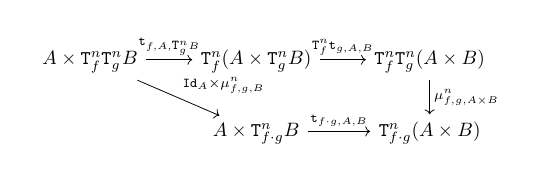
\begin{tikzpicture}[baseline= (a).base]
                    \node[scale=.7] (a) at (0,0){
                \begin{tikzcd}
                    A \times \Tn{f}{\Tn{g}{B}} 
                    \arrow [r, "\tstrength{f}{A}{\Tn{g}{B}}"]
                    \arrow [dr, "\Id{A} \times \bindn{f}{g}{B}"]
                    & 
                    \Tn{f}{(A \times \Tn{g}{B})} 
                    \arrow [r, "\Tn{f}{\tstrength{g}{A}{B}}"]
                    & 
                    \Tn{f}{\Tn{g}{(A \times B)}} 
                    \arrow [d, "\bindn{f}{g}{A \times B}"]
                    \\
                    &
                    A \times \Tn{f \dot g}{B}  
                    \arrow [r, "\tstrength{f \dot g}{A}{B}"] 
                    &
                    \Tn{f \dot g}({A \times B)}
                \end{tikzcd}};
            \end{tikzpicture}
            \end{minipage}
            \quad
            \begin{minipage}{.45\textwidth}
                \centering
                \scalebox{.75}{\parbox{\linewidth}{%
                    \begin{align*}
                        & (\tstrengthn{(f\dot g)}{A}{B}\after (\Id{A}\times \bindn{f}{g}{B}))\ev \\
                        & = (\tstrengthz{((f\ev)\dot (g\ev))}{(A\ev)}{(B\ev)}\after (\Id{A\ev}\times \bindn{(f\ev)}{(g\ev)}{(B\ev)}))\\
                        & = \bindz{(f\ev)}{(g\ev)}{(A\times B)\ev}\after\Tz{f\ev}{(\tstrengthz{(g\ev)}{(A\ev)}{(B\ev)})}\after\tstrengthz{(f\ev)}{(A\ev)}{\Tz{g\ev}{(B\ev)}}\\
                        & = (\bindn{f}{g}{(A\times B)}\after\Tn{f}{(\tstrengthn{g}{A}{B})}\after\tstrengthn{f}{A}{\Tn{g}{(B)}})\ev
                    \end{align*}
                }}
            \end{minipage}
        \end{framed}
    
        \begin{framed}
            \centering
            \textbf{Commutativity with Unit}
    
            \begin{minipage}{.45\textwidth}
                \centering
                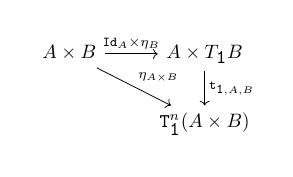
\begin{tikzpicture}[baseline= (a).base]
                    \node[scale=.7] (a) at (0,0){
                
                    \begin{tikzcd}
                        A \times B
                        \arrow [r, "\Id{A} \times \point{B}"]
                        \arrow [rd, "\point{A \times B}"]
                        &
                        A \times \tob 
                        \arrow [d, "\tstrength{\1}{A}{B}"]
                        \\
                        &
                        \Tn{\1}{(A \times B)}
                    \end{tikzcd}
                };
            \end{tikzpicture}
            \end{minipage}
            \quad
            \begin{minipage}{.45\textwidth}
                \centering
                \scalebox{.75}{\parbox{\linewidth}{%
                \begin{align*}
                    (\tstrengthn{\1}{A}{B}\after(\Id{A}\times \pointn{A}))\ev & = \tstrengthz{\1}{(A\ev)}{(B\ev)}\after(\Id{A\ev}\times \pointz{A\ev})\\
                    & = \pointz{A\ev\times B\ev}\\
                    & = (\pointn{A\times B})\ev
                \end{align*}
                }}
            \end{minipage}
        \end{framed}
    
        \begin{framed}
            \centering
            \textbf{Commutativity with $\alpha$}

            Let $\alpha_{A, B, C} = \pr{\p\after\p}{\pr{\pp\after\p}{\pp}}: ((A \times B) \times C) \rightarrow (A \times (B \times C))$
    
    
            \begin{minipage}{.45\textwidth}
                \centering
                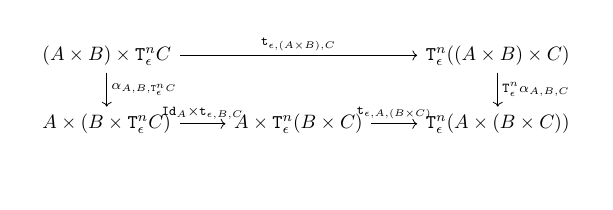
\begin{tikzpicture}[baseline= (a).base]
                    \node[scale=.7] (a) at (0,0){
                    \begin{tikzcd}
                        (A\times B)\times \Tn{\e}{C} 
                        \arrow [rr, "\tstrength{\e}{(A\times B)}{C}"]
                        \arrow [d, "\alpha_{A, B, \Tn{\e}{C}}"]
                        & & \Tn{\e}{((A \times B)\times C)}
                        \arrow [d, "\Tn{\e}{\alpha_{A, B, C}}"]
                        \\
                        A \times (B \times \Tn{\e}{C}) 
                        \arrow [r, "\Id{A}\times\tstrength{\e}{B}{C}"]
                        &
                        A\times\Tn{\e}{(B \times C)} 
                        \arrow [r, "\tstrength{\e}{A}{(B \times C)}"]
                        & \Tn{\e}{(A \times (B \times C))}
                        \\
                    \end{tikzcd}
                };
            \end{tikzpicture}
            \end{minipage}
            \quad
            \begin{minipage}{.45\textwidth}
                \centering
                \scalebox{.75}{\parbox{\linewidth}{%
                \begin{align*}
                    & (\Tn{f}{\alpha_{A, B, C}}\after\tstrengthn{f}{A\times B}{C})\ev \\
                    & = \Tz{f\ev}{\alpha_{A\ev, B\ev, C\ev}} \after\tstrengthz{(f\ev)}{(A\times B)\ev}{(C\ev)}\\
                    & = \tstrengthz{(f\ev)}{(A\ev)}{(B\ev\times C\ev)}\after(\Id{A\ev}\times \tstrengthz{(f\ev)}{(B\ev)}{(C\ev)})\after\alpha_{A\ev, B\ev, C\ev}\\
                    & = (\tstrengthn{f}{A}{(B\times C)}\after(\Id{A}\times \tstrengthn{f}{B}{C})\after\alpha_{A, B, C})\ev\\
                \end{align*}            
                }}
            \end{minipage}
        \end{framed}
\end{framed}

    \caption{The tensor strength laws can be proved component wise from the strength of the monad $\Tz{}{}$}
    \label{TensorStength}
\end{figure}



\subsection{Subeffecting}
Given a collection of subeffecting natural transformation in $\set$, $\deno{\e_1\subeffectz \e_2}: \quad \Tz{\e_1}{} \rightarrow \Tz{\e_2}{}$ we can form subeffect natural transformations in $[E^n, \set]$ as seen in figure \ref{SubEffecting}. This natural transformation has all the required properties. These are proved in figure \ref{SubeffectProperties}.

\begin{figure}
    \begin{framed}
        \centering\textbf{Subeffect Natural Transformation}
    
        \begin{align*}
            \deno{f\subeffectn g}:&\quad\Tn{f}{}\rightarrow \Tn{g}{}\\
            \deno{f\subeffectn g} A \ev:&\quad\Tn{f\ev}{(A\ev)}\rightarrow \Tn{g\ev}{(B\ev)}\\
            =&\quad \deno{f\ev\subeffectz g\ev}A\ev
        \end{align*}
    \end{framed}
    \caption{Definition of subeffecting natural transformations}
    \label{SubEffecting}
\end{figure}

\begin{figure}
    \begin{framed}
        \centering\textbf{Subeffect Natural Transformation Properties}

        \begin{framed}
            \centering
            \textbf{Naturality}
            
            \begin{tikzcd}[column sep=large]
                \Tz{f\ev}{A\ev}
                \arrow{r}{\deno{f\ev\subeffectz g\ev}A\ev}
                \arrow{d}{\Tz{f\ev}{m\ev}}
                &
                \Tz{g\ev}{A\ev}
                \arrow{d}{\Tz{g\ev}{m\ev}}
                \\
                \Tz{f\ev}{B\ev}
                \arrow{r}{\deno{f\ev\subeffectz g\ev}B\ev}
                &
                \Tz{g\ev}{B\ev}
            \end{tikzcd}
        \end{framed}

        \begin{framed}
            \centering
            \textbf{Commutes With Tensor Strength}




    
            \begin{minipage}{.45\textwidth}
                \centering
                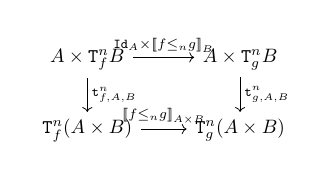
\begin{tikzpicture}[baseline= (a).base]
                    \node[scale=.7] (a) at (0,0){\begin{tikzcd}
                        A \times \Tn{f}{B} \arrow [r, "\Id{A} \times \dsen{f}{g}_B"] \arrow [d, "\tstrengthn{f}{A}{B}"] &
                        A \times \Tn{g}{B} \arrow [d, "\tstrengthn{g}{A}{B}"] \\
                        \Tn{f}{(A \times B)} \arrow [r, "\dsen{f}{g}_{ A \times B}"] &
                        \Tn{g}{(A \times B)} 
                    \end{tikzcd}
                    };
            \end{tikzpicture}
            \end{minipage}
            \quad
            \begin{minipage}{.45\textwidth}
                \centering
                \scalebox{.75}{\parbox{\linewidth}{%
                \begin{align*}
                    & (\tstrengthn{g}{A}{B}\after(\Id{A}\times \db{f\subeffectn g}_B))\ev \\
                    &= \tstrengthz{(g\ev)}{(A\ev)}{(B\ev)}\after(\Id{A\ev}\times \db{f\ev \subeffectz g\ev}_{B\ev})\\
                    & = \db{f\ev \subeffectz g\ev}_{(A\times B)\ev} \after\tstrengthz{(f\ev)}{(A\ev)}{(B\ev)}\\
                    & = (\db{f \subeffectn g}_{(A\times B)} \after\tstrengthn{f}{A}{B})\ev\\
                \end{align*}
                }}
            \end{minipage}
        \end{framed}

        \begin{framed}
            \centering
            \textbf{Commutes with Join}

            \begin{minipage}{.45\textwidth}
                \centering
                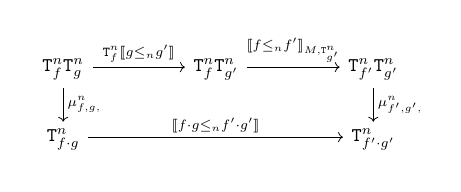
\begin{tikzpicture}[baseline= (a).base]
                    \node[scale=.7] (a) at (0,0){
                    \begin{tikzcd}
                        \Tn{f}{\Tn{g}{}} 
                        \arrow [rr, "\Tn{f}{\deno{g\subeffectn g'}
                        }"]
                        \arrow [d, "\bindn{f}{g}{}"]
                        &  &
                        \Tn{f}{\Tn{g'}{}}
                        \arrow [rr, "\db{f \subeffectn f'}_{M, \Tn{g'}{}}"]
                        & &
                         \Tn{f'}{\Tn{g'}{}} 
                         \arrow [d, "\bindn{f'}{g'}{}"]
                         \\
                        \Tn{f\dot g}{}
                        \arrow [rrrr, "\deno{f\dot g\subeffectn f'\dot g'}"]
                        & &
                         & &
                        \Tn{f'\dot g'}{}
                    \end{tikzcd}                    
                    };
            \end{tikzpicture}
            \end{minipage}
            \quad
            \begin{minipage}{.45\textwidth}
                \centering
                \scalebox{.75}{\parbox{\linewidth}{%
                \begin{align*}
                    & (\dsen{f\dot g}{f'\dot g'}_A\after\bindn{f}{g}{A})\ev \\ & = \dsez{(f\ev)\dot(g\ev)}{(f'\ev)\dot (g\ev)}_{A\ev}\after\bindz{(f\ev)}{(g\ev)}{(A\ev)}\\
                    & = \bindz{(f\ev)}{(g\ev)}{(A\ev)}\after\dsez{f\ev}{f'\ev}_{\Tz{g'\ev}{(A\ev)}}\after \Tz{f\ev}{\dsez{g\ev}{g'\ev}}_{(A\ev)}\\
                    &= \bindn{f}{g}{A}\after\dsen{f}{f'}_{\Tn{g'}{A}}\after\Tn{f}{\dsen{g}{g'}}_A
                \end{align*}
                }}
            \end{minipage}
        \end{framed}
        
    \end{framed}
    \caption{The required properties of the subeffect natural transformations can be proved component-wise from the appropriate of the subeffect natural transformation on $\set$.}
    \label{SubeffectProperties}
\end{figure}

\section{Re-indexing Functors}
\label{ReindexingFunctorProperties}
For a function $\theta: E^m \rightarrow E^n$ , the re-indexing functor $\theta\star$ is defined as follows:

\begin{align*}
    \theta\star:\quad& [E^n, \set] \rightarrow [E^m, \set]\\
    \theta\star(A)\emv=&\quad A(\theta (\emv))\\
    f:\quad& A \rightarrow B \in[E^n, \set]\\
    \theta\star(f)\emv =&\quad f(\theta(\emv)): A(\theta(\emv)\rightarrow B(\theta(\emv)))
\end{align*}

This functor preserves all the S-category properties.
These can be seen in figures \ref{PreservesCCC}-\ref{PreservesSubtypingSubeffecting}


\begin{figure}
    \centering
        \begin{framed}
            \centering\textbf{$\theta\star$ is Cartesian Closed}

            \begin{minipage}{.45\linewidth}
                \begin{align*}
                    (\theta\star(A\times B))\ev & = (A\times B)(\theta\ev)\\
                    & = (A(\theta \ev)\times B(\theta\ev))\\
                    & = (\theta\star A\times \theta\star B)\ev\\
                \end{align*}              
            \end{minipage}
            \quad
            \begin{minipage}{.45\linewidth}
                \begin{align*}
                    (\theta\star \p)\ev & = \p(\theta\ev)\\
                    & = \p \qt{Constant function}\\
                    & = \p\ev
                \end{align*}                
            \end{minipage}


            \begin{minipage}{.45\linewidth}
                \begin{align*}
                    (\theta\star \pp)\ev & = \pp(\theta\ev)\\
                    & = \pp \qt{Constant function}\\
                    & = \pp\ev
                \end{align*}                
            \end{minipage}
            \quad
            \begin{minipage}{.45\linewidth}
                \begin{align*}
                    (\theta\star\pr{f}{g})\ev & = (\pr{f}{g})(\theta\ev)\\
                    & = \pr{f(\theta\ev)}{g(\theta\ev)}\\
                    &= \pr{\theta\star f}{\theta\star g}\ev
                \end{align*}
            \end{minipage}

            \begin{minipage}{.45\linewidth}
                \begin{align*}
                    (\theta\star(A^B))\ev & = (A^B)(\theta\ev)\\
                     & = (A (\theta\ev))^{(B (\theta\ev))}\\
                     & = (\theta\star A)^{(\theta\star B)}\ev\\
                \end{align*}                
            \end{minipage}
            \quad
            \begin{minipage}{.45\linewidth}
                \begin{align*}
                (\theta\star \app)\ev & = \app(\theta\ev)\\
                & = \app \qt{Constant fn}\\
                & = \app\ev
            \end{align*}
            \end{minipage}

        \begin{minipage}{.45\linewidth}
            \begin{align*}
                (\theta\star\cur{f})\ev & = \cur{f}(\theta\ev)\\
                & = \cur{f(\theta\ev)}\\
                & = \cur{\theta\star f}
            \end{align*}             
        \end{minipage}
        \quad
        \begin{minipage}{.45\linewidth}
            \begin{align*}
                (\theta\star \1)\ev & = \1(\theta\ev)\\
                & = \1 \\
                & = \1 \ev\\
            \end{align*}
        \end{minipage}      
        
        \begin{minipage}{\linewidth}
            \begin{align*}
                (\theta\star\term{A})\ev & = \term{A}(\theta\ev)\\
                & = \term{A(\theta\ev)}\\
                & = \term{\theta\star A}\ev
            \end{align*}
        \end{minipage}        
    \end{framed}
    
    \caption{Proof of the CCC-preserving property of re-indexing functors.}
    \label{PreservesCCC}
\end{figure}

\begin{figure}
    \centering
    \begin{framed}
        \centering\textbf{$\theta\star$ Preserves Co-products}

        \begin{minipage}{.45\textwidth}
            \begin{align*}
                (\theta\star(\1 + \1))\ev & = (\1 + \1)(\theta\ev)\\
                & = (\1 + \1)\qt{Constant function}\\
                & = (\1 + \1)\ev
            \end{align*}
        \end{minipage}
        \quad
        \begin{minipage}{.45\textwidth}
            \begin{align*}
                (\theta\star\inl )\ev & = \inl(\theta\ev)\\
                & = \inl \qt{Constant Fn}\\
                & = \inl \ev
            \end{align*}
        \end{minipage}

        \begin{minipage}{.45\textwidth}
            \begin{align*}
                (\theta\star\inr )\ev & = \inr(\theta\ev)\\
                & = \inr \qt{Constant Fn}\\
                & = \inr \ev
            \end{align*}
        \end{minipage}
        \quad
        \begin{minipage}{.45\textwidth}
            \begin{align*}
                (\theta\star [f, g])\ev & = [f, g](\theta\ev)\\
                & = [f (\theta\ev), g(\theta\ev)]\\
                & = [\theta\star f, \theta\star g]\ev\\
            \end{align*}
        \end{minipage}        
    \end{framed}
    
    \caption{Proof that re-indexing functors preserve the $\1 + \1$ co-product.}
    \label{PreservesCoProduct}
\end{figure}



\begin{figure}
    \centering
    \begin{framed}
        \centering\textbf{$\theta\star$ Preserves the Graded Monad}

        \begin{minipage}{.45\textwidth}
            \begin{align*}
                (\theta\star\Tn{f}{A})\ev & = \Tn{f}{A}(\theta\ev) \\
                & = \Tz{(f(\theta\ev))}{(A(\theta\ev))}\\
                & = (\Tm{(f\after\theta)}{\theta\star A})\ev\\
            \end{align*}
        \end{minipage}
        \quad
        \begin{minipage}{.45\textwidth}
            \begin{align*}
                (\theta\star\pointn{A})\ev & = \pointn{A}(\theta\ev) \\
                & = \pointz{A(\theta\ev)}\\
                & = \pointm{\theta\star A}\ev\\
            \end{align*}
        \end{minipage}

        \begin{minipage}{.45\textwidth}
            \begin{align*}
                (\theta\star \bindn{f}{g}{A})\ev & = \bindn{f}{g}{A}(\theta\ev)\\
                & = \bindz{f(\theta\ev)}{g(\theta\ev)}{A(\theta\ev)}\\
                & = \bindm{f\after\theta}{g\after\theta}{\theta\star(A)}(\ev)
            \end{align*}
        \end{minipage}
        \quad
        \begin{minipage}{.45\textwidth}
            \begin{align*}
                (\theta\star \tstrengthn{f}{A}{B})\ev & = \tstrengthn{f}{A}{B}(\theta \ev)\\
                & = \tstrengthz{(f(\theta\ev))}{(A(\theta\ev))}{(B(\theta\ev))}\\
                & = \tstrengthm{f\after\theta}{\theta\star A}{\theta\star B}\ev\\
            \end{align*}
        \end{minipage}        
    \end{framed}
    
    \caption{Re-indexing functors preserve the graded monad structure}
    \label{GradedMonadPreserved}
\end{figure}

\begin{figure}
    \begin{framed}
        \centering\textbf{$\theta\star$ preserves Ground Subtyping and Subeffecting}

        \begin{minipage}{.45\textwidth}
            \begin{align*}
                \theta\star(\deno{A\subtypeg B})\ev  & = \deno{A\subtypeg B}(\theta\ev)\\
                & = \deno{A\subtype B} \qt{Constant Function}\\
                & = \deno{A\subtype B} \ev\\
            \end{align*}
        \end{minipage}
        \quad
        \begin{minipage}{.45\textwidth}
            \begin{align*}
                (\theta\star(\dsen{f}{g} A))\ev & = (\dsen{f}{g} A)(\theta \ev)\\
                & = (\dsen{f(\theta\ev)}{g(\theta\ev)}(A(\theta\ev)))\\
                & = (\dsem{\theta\star f}{\theta\star g} (\theta\star A)) \ev\\
            \end{align*}
        \end{minipage}
    \end{framed}
    \caption{Re-indexing functors preserve the ground subtyping and subeffecting morphisms.}
    \label{PreservesSubtypingSubeffecting}
\end{figure}


\subsection{Quantification}
We need to define $\allEn: [E^{n+1}, \set]\rightarrow[E^n, \set]$

So
\begin{align*}
    (\allEn A)\env =&\quad \Pi_{\e\in E} A(\env, \e)\\
    m:&\quad A\rightarrow B\\
    (\allEn m):&\quad \allEn A\rightarrow \allEn B\\
    (\allEn m)\env =&\Pi_{\e\in E} m(\env, \e)\\
\end{align*}

\end{document}


\end{document}